%##################################################################################\textbf{}

\documentclass[12pt,a4paper,twoside,varwidth = false , border = 2pt]{report}
%\documentclass[varwidth=false, border=2pt]{standalone}
%\documentclass[12pt,a4paper,oneside]{report}
%\documentclass[tikz, border=3mm]{standalone}
\usepackage{graphicx}
%\usepackage[ngerman, english]{babel} %-- uncomment this to get english titles
\usepackage[ngerman]{babel}
\usepackage{german,a4}
%\usepackage{picins}
%\usepackage{epsfig}
\usepackage{fancyhdr}			% for nice header and footer
\usepackage{hyperref}			% references in pdf
\usepackage[sf]{titlesec}	%customization of \chapter Titles for appendices
\usepackage{textcomp}
\usepackage{makeidx}
\usepackage{ngerman}			% german Umlauts
\usepackage[utf8]{inputenc}
\usepackage{booktabs}                               % necessary for tabulars
\usepackage[squaren]{SIunits}
\usepackage[numbers,square]{natbib}
\usepackage{tikz}
\usetikzlibrary{matrix,chains,positioning,decorations.pathreplacing,arrows,backgrounds}
\usepackage{pgfplots}
\usepackage{float}
\usetikzlibrary{matrix,arrows.meta,positioning}
\usepackage{caption}
\usepackage{wrapfig}
\usepackage{subcaption}
%\graphicspath{{./Bilder/}}

%%%%%%%%%%%%%%%%%%%%%%%%%%%%%%%%%%%%%%%%%%%%%%%%%%%

\usepackage[utf8]{inputenc}
\usepackage{amsmath, amssymb, latexsym}

\usepackage{tikz}
\usetikzlibrary{decorations.pathreplacing}
\usetikzlibrary{fadings}	

%%%%%%%%%%%%%%%%%%%%%%%%%%%%%%%%%%%%%%%%%%%%%%%%%%%





%\usetikzlibrary{matrix,chains,positioning,decorations.pathreplacing,arrows}




%\usepackage{wrapfig} 
%\usepackage[pdftex]{graphicx}
%\usepackage{ifthen}  
%\usepackage{booktabs} % fancy tables
%\usepackage[titletoc]{appendix} % custom naming of appendices
\usepackage{amssymb, amsmath, amsthm} % for equations & eqref
%\usepackage{listings} \lstset{basicstyle=\tiny\ttfamily, numbers=left, escapeinside={(*}{*)}, captionpos=b}
%\usepackage{dirtree}

%get bigger \par with one empty line
\newcommand{\mypar}{\par\medskip}

%TODO line
\newcommand{\writeTodo}{1}
\newcommand{\todo}[1]{
	\ifdefined \writeTodo
		\mypar\textbf{\textcolor{KITgreen}{TODO: }\textcolor{red}{#1}}\mypar
	\fi
} 
 
%\theoremstyle{plain}% default
\theoremstyle{definition}
\newtheorem{definition}{Definition}

% Abbkürzungsverzeichnis einfügen
%%%%%%%%%%%%%%%%%%%%%%%%%%%%%%%%%%%%%%%%%%%%%%%%%%%%%%%%% 
\usepackage{nomencl}
\let\abbrev\nomenclature
\renewcommand{\nomname}{Abkürzungsverzeichnis}
\setlength{\nomlabelwidth}{.25\hsize}
\renewcommand{\nomlabel}[1]{#1 }%\dotfill}

\setlength{\nomitemsep}{-\parsep}
\makenomenclature
\newcommand{\markup}[1]{\underline{#1}} 

% Farben
\usepackage{color}
\definecolor{KITgreen}{rgb}{0, .61, .51} 
\definecolor{KITbluegrey}{rgb}{.27, .39, .67} 
\definecolor{KITgrey}{rgb}{.49, .49, .49} 

% =====================================================
% Dokumenten-Platzhalter
% =====================================================
% =====================================================
% Dokumenten Platzhalter
% =====================================================


\newcommand{\titelderarbeit}{Implementierung und Evaluation von Systolic Arrays für maschinelles Lernen}
\newcommand{\artderarbeit}{Bachelorarbeit}

\newcommand{\diplomandprefix}{cand. el.}
\newcommand{\diplomand}{Ahmet Narin}

\newcommand{\betreuerA}{Tim Hotfilter}
\newcommand{\betreuerB}{ }

 
%\newcommand{\nameprefix}{}{}    %use no nameprefix 
\newcommand{\nameprefix}{M. Sc. }
\newcommand{\docauthor}{Andreas Lauber}

\newcommand{\nameprefixb}{}{}    %use no nameprefix 
%\newcommand{\nameprefixb}{Dipl.-Ing.}  
\newcommand{\docauthorb}{}

\newcommand{\nameprefixc}{}{}    %use no nameprefix 
%\newcommand{\nameprefixc}{Dipl.-Ing.}
\newcommand{\docauthorc}{}

%\newcommand{\betreuerA}{nn}
%\newcommand{\betreuerB}{nn}
\newcommand{\abgabe}{17 Februar 2020}
\newcommand{\versionierungsnr}{v1.0}
\newcommand{\fussnoteninhalt}{}
\newcommand{\leerzeichen}{ }

%% english version
%\newcommand{\Dachorganisation}{Karlsruhe Institute of Technology - KIT}
%\newcommand{\Institut}{Institute for Information Processing 
%												Technology - ITIV}
												
% deutsche version
\newcommand{\Dachorganisation}{Karlsruher Institut für Technologie - KIT}
\newcommand{\Institut}{Institut für Technik der Informationsverarbeitung - ITIV}

% ====================================================
% Formatierung des Dokuments
% ====================================================


%\usepackage{color}
%\usepackage{helvet}

% =====================================================
% Seite einrichten
% =====================================================
\setlength{\textwidth}{160mm} \setlength{\textheight}{235mm}
\setlength{\oddsidemargin}{5mm}
%pagelayout: (1in=25,4mm), default offset of page origin: 1in x 1in
%     25,4+5=30,4mm       160mm          19,6mm
%  |                   sadfasdfasdfasdf          |
\setlength{\evensidemargin}{-5,8mm} 
%     25,4-5,8= 19,6mm    160mm          30,4mm
%  |                   sadfasdfasdfasdf          |
\setlength{\topmargin}{0mm} \setlength{\voffset}{-15mm}
\setlength{\headsep}{12mm} \setlength{\footskip}{15mm}
\setlength{\headheight}{15.5pt}

% =====================================================
% sonstige Einstellungen
% =====================================================
%\flushbottom % Textfluss schoen unten ausrichten
\footnotesep12pt % Abstand Text / Fussnote
%\setlength{\parindent}{0pt} \setlength{\abovecaptionskip}{-6pt}
%\setlength{\belowcaptionskip}{0pt} \setlength{\intextsep}{18pt}
%\renewcommand{\baselinestretch}{1.2} % Zeilenabstand
\setcounter{secnumdepth}{4}
\newcommand{\p}[1]{\texttt{#1}}
\nonfrenchspacing

% =====================================================
% Kopf- und Fusszeile formatieren
% =====================================================
\pagestyle{fancy}
\fancyhead{}
\makeatletter
\if@twoside
	\fancyhead[LO]{\sf{\rightmark}}
	\fancyhead[RE]{\sf{\leftmark}}
	\fancyfoot[LE]{\setlength{\unitlength}{1mm}
		\begin{picture}(0,0) \put(0,-2){
			%
\includegraphics[height=0.6cm,width=0.6cm]{98_images/ITIVlogo.png}
		} \end{picture}
		%\put(9,2){\scriptsize\sf{\Institut}}\put(9,-2){\scriptsize\sf{\Dachorganisation}}}
		\put(0,2){\scriptsize\sf{\Institut}}\put(0,-2){\scriptsize\sf{\Dachorganisation}}}

\else
	\fancyhead[LO]{\sf{\leftmark}}
	\fancyfoot[LO]{\setlength{\unitlength}{1mm} 
		\begin{picture}(0,0) \put(0,-2){
			% 
\includegraphics[height=0.6cm,width=0.6cm]{98_images/ITIVlogo.png}
		} \end{picture}
		%\put(9,2){\scriptsize\sf{\Institut}}\put(9,-2){\scriptsize\sf{\Dachorganisation}}}
		\put(0,2){\scriptsize\sf{\Institut}}\put(0,-2){\scriptsize\sf{\Dachorganisation}}}
\fi
\fancyhead[LE, RO]{\sf{\thepage}}
\makeatother

\cfoot{}
\fancyfoot[RO]{\footnotesize\sf{\titelderarbeit}}
\renewcommand{\headrulewidth}{0.4pt}
\renewcommand{\footrulewidth}{1.0pt}

% ====================================================
% Kopf- und Fusszeile fuer "plain"-Format ueberschreiben
% ====================================================
\makeatletter
\if@twoside
	\fancypagestyle{plain}{%
	\fancyhf{}
	\fancyfoot[LE]{\setlength{\unitlength}{1mm}
		\begin{picture}(0,0) \put(0,-2){
			%
\includegraphics[height=0.6cm,width=0.6cm]{98_images/ITIVlogo.png}
		} \end{picture}
		%\put(9,2){\scriptsize\sf{\Institut}}\put(9,-2){\scriptsize\sf{\Dachorganisation}}}
		\put(0,2){\scriptsize\sf{\Institut}}\put(0,-2){\scriptsize\sf{\Dachorganisation}}}
	\cfoot{}
	\fancyfoot[RO]{\footnotesize\sf{\titelderarbeit}}
	\renewcommand{\headrulewidth}{0pt}
	\renewcommand{\footrulewidth}{1.0pt}}
\else
	\fancypagestyle{plain}{%
	\fancyhf{}
	\fancyfoot[L,C,R]{\setlength{\unitlength}{1mm}
	\begin{picture}(0,0) \put(0,-2){
		%
\includegraphics[height=0.6cm,width=0.6cm]{98_images/ITIVlogo.png}
	} \end{picture}
	%\put(9,2){\scriptsize\sf{\Institut}}\put(9,-2){\scriptsize\sf{\Dachorganisation}}}
	\put(0,2){\scriptsize\sf{\Institut}}\put(0,-2){\scriptsize\sf{\Dachorganisation}}}
	\cfoot{}
	\rfoot{\footnotesize\sf{\titelderarbeit}}
	\renewcommand{\headrulewidth}{0pt}
	\renewcommand{\footrulewidth}{1.0pt}}
\fi

%makes the index do not remove!
\makeindex

\hypersetup{
	%pdftex %schon gesetzt
	pdfauthor = \docauthor,
	%pagebackref,%schon gesetzt
	colorlinks=true,
	linkcolor=black,
	citecolor=black,
	urlcolor=black
	}

\providecommand{\e}[1]{\ensuremath{\times 10^{#1}}}

% =====================================================
% Inhalt der Titelseite definieren
% =====================================================

\makeindex
\newcommand{\Idx}[1]{#1 \index{#1}}

\hyphenation{
EVITA
}

% =====================================================
% Zeichen für Copyright, Trademark, Registerd, ...
% =====================================================
\def\TReg{\textsuperscript{\textregistered}}
\def\TCop{\textsuperscript{\textcopyright}}
\def\TTra{\textsuperscript{\texttrademark}}

% =====================================================
% selbs definierte Zeichen
% =====================================================
\def\zB{z.\,B. }
\def\uvm{u.\,v.\,m.}
\begin{document}

% =====================================================
% Put Titel in English
% ===================================================== 
%
% Inhalt der Titelseite definieren
\pagestyle{empty}
\pagenumbering{roman}
\setcounter{page}{1}

\begin{titlepage}

\begin{minipage}{15cm}
\linespread{1.2}

\begin{tabular}{lr}
\begin{minipage}{0.2\linewidth}

\includegraphics[height=1cm]{98_images/kit.png}
\end{minipage}
&
\begin{minipage}{0.8\linewidth}
\large
%\center
\vspace{7mm}
\begin{flushleft}
\Dachorganisation
\end{flushleft}
\end{minipage}
\\
\\
\begin{minipage}{0.2\linewidth}
\includegraphics[height=1cm]{98_images/ITIVLogo.png}
\end{minipage}
&
\begin{minipage}{0.8\linewidth}
\large
%\center
\vspace{7mm}
\begin{flushleft}
\Institut\\
\end{flushleft}
\end{minipage}
\\
\end{tabular}

\vspace{3cm}

\begin{center}
\Huge
\bfseries  \titelderarbeit
\end{center}

\vspace{1cm}
\begin{center}
\large 
\subtitelderarbeit 
\vspace{1cm}
%\Large
%\textbf{\diplomandprefix\ \diplomand}

\vspace{1cm}
%\Large
%%Berichtsbezeichnung und ID Nummer
 Version 
\versionierungsnr\\
\abgabe%\textbf{\abgabe}
\end{center}
%
\vspace{2.5cm}

\begin{tabular}{rcl}
\bfseries Head of Institute:
&& Prof. Dr.-Ing. J. Becker\\
&& Prof. Dr. rer. nat  W. Stork\\
&& Prof. Dr.-Ing. Eric Sax\\
 \\
	\bfseries Author:         && \nameprefix \leerzeichen \docauthor \\
											      && \nameprefixb \leerzeichen \docauthorb\\
														&& \nameprefixc \leerzeichen \docauthorc \\
											      \end{tabular}											
											      
\end{minipage}
\end{titlepage}
\pagestyle{fancy}
%    \parindent=0pt
%    %\sloppypar
%    \linespread{1.2}
%    \thispagestyle{plain}
%    %\frontmatter
%    %\maketitle

% =====================================================
% Put Titel in Deutsch
% ===================================================== 

% Inhalt der Titelseite definieren
\pagestyle{empty}
\pagenumbering{roman}
\setcounter{page}{1}

\begin{titlepage}

\begin{minipage}{15cm}
\linespread{1.2}

\begin{tabular}{lr}
\begin{minipage}{0.3\linewidth}

\includegraphics[height=2cm]{98_images/kit.png}
\end{minipage}
&
\begin{minipage}{0.7\linewidth}
\large
\center
Karlsruhe Institute of Technology\\
Fakultät für Elektrotechnik
\end{minipage}
\\
\\
\begin{minipage}{0.3\linewidth}
\includegraphics[height=2cm]{98_images/ITIVLogo.png}
\end{minipage}
&
\begin{minipage}{0.7\linewidth}
\large
\center
Institut für Technik der Informationsverarbeitung (ITIV)\\
\end{minipage}
\\
\end{tabular}

% #################################################################
% ### If the Title is very long reduce vspace to less than 2cm
% #################################################################
\vspace{1.5cm}

% #################################################################

\begin{center}
\Huge
\bfseries  \titelderarbeit
\end{center}

\vspace{1cm}
\begin{center}
\large 
\artderarbeit ~von\\
\vspace{1cm}
\Large
\textbf{\diplomandprefix\ \diplomand}

\vspace{1cm}
\Large
\textbf{\abgabe}
\end{center}
%
\vspace{2.5cm}

\begin{tabular}{rcl}
\bfseries Institutsleitung: 
&& Prof. Dr.-Ing. Dr. h.c. J. Becker\\
&& Prof. Dr.-Ing. Eric Sax\\
&& Prof. Dr. rer. nat  W. Stork\\

 \\
	\bfseries Betreuer:       &&\nameprefix  \betreuerA \\
											      && \betreuerB \\
\end{tabular}											
\end{minipage}
\end{titlepage}
    \parindent=0pt
    %\sloppypar
    \linespread{1.2}
    \thispagestyle{plain}
    %\frontmatter
    %\maketitle
    %\cleardoublepage
    
% =====================================================
% Abstract
% =====================================================     
	\begin{abstract}
		Unser Alltag und Geschäftsleben wird immer mehr von machine Learning (ML) beeinflusst. Beispiele für den Einsatz begegnen uns im täglichen Leben bereits überall. Einige davon sind Gesichts-und Spracherkennung, personalisierte Produktempfehlungen bei Amazon oder Börsenprognose für Spekulanten etc. Aber auch in sicherheitskritischen Systeme wie autonomes Fahren wird das ML-Verfahren eingesetzt. Das Ziel von dieser Arbeit ist, dass die Datenverarbeitung von solchen sicherheitskritischen Anwendungen beschleunigt  und parallele Multiplikation-und Akkumulations-Operationen ausgeführt werden. Somit wird die Rechenleistung von Embedded Systems und IoT-Geräten erhöht und 


\cleardoublepage

\chapter*{Urheberrecht}

ARM\TReg, AMBA\TReg, AXI\TTra, Cortex\TTra, TrustZone\TTra, SecurCore\TTra  , DSTREAM\TTra und weitere im Text erwähnte ARM-Produkte sowie die entsprechenden Logos sind Marken oder eingetragene Marken der Advanced RISC Machines Ltd.\par
\vspace{0.5cm}
Xilinx\TReg, Zynq\TTra und weitere im Text erwähnte Xilinx-Produkte sowie die entsprechenden Logos sind Marken oder eingetragene Marken der Xilinx Inc.\par
\vspace{0.5cm}
		
	\end{abstract}
	\cleardoublepage
% =====================================================
% Signaturepage
% ===================================================== 
    \chapter*{}
\begin{flushleft}
\vspace{11cm}
Erklärung\\[1cm]
Ich versichere hiermit, dass ich meine Bachelorarbeit selbständig und unter Beachtung der Regeln zur Sicherung guter wissenschaftlicher Praxis im Karlsruher Institut für Technologie (KIT) in der aktuellen Fassung angefertigt habe. \\
Ich habe keine anderen als die angegebenen Quellen und Hilfsmittel benutzt und wörtlich oder inhaltlich übernommene Stellen als solche kenntlich gemacht.\\[1cm]

Karlsruhe, den \abgabe\\[1cm]
\end{flushleft}

\begin{center}
---------------------------------\\
%\diplomand
\end{center}

	\cleardoublepage
% =====================================================
% TOC
% ===================================================== 
    \tableofcontents
    %\clearpage
    %\cleardoublepage

% =====================================================
% Main Chapters
% ===================================================== 
    %\mainmatter
    \pagenumbering{arabic}
    \setcounter{page}{1}
    \pagestyle{fancy}
 	\normalsize

    

    \chapter{Einleitung}
    \label{ch:Einleitung} 
    \section{Motivation}\label{sec:?}   
    
    %\cleardoublepage   
    Neue innovative Projekte wie autonomes Fahren oder auch kommenden neue Technologien in der Zukunft und industrielle Automatisierung  müssen immer mehr mit umfangreicher Datenmenge umgehen. ML-Methoden werden in solchen Anwendungen häufig verwendet, damit die Daten analysiert werden können bzw. die Maschinen etwas neues aus den Daten ohne explizite Programmierung lernen. Insbesondere im Kontext von Echtzeitsystemen stellt sich die Latenz während der Datenverarbeitung als Flaschenhals dar.\\
    \\
    Die CPU-Hardwarearchitektur kann dieses Problem leider nicht lösen, da CPUs für allgemeinen Gebrauch vorgesehen sind. GPU (graphics processing unit) ist für solchen rechenintensiven Anwendungen besser geeignet, um die Datenverarbeitung zu beschleunigen. Aber sie verbrauchen viel Energie und für mobile Geräte und Embedded Systems nicht einsetzbar. Eine spezielle Hardwarearchitektur soll für diesen Zweck eingesetzt werden. Es soll wenig Strom verbrauchen und trotz dieser Anforderung auch schnell und mehrfache vorkommende Multiplikation-und Addition Operationen bearbeiten. \\
    \\
	Das \textbf{FPGA} (field-programable gate array) kann diese Anforderungen erfüllen. Das FPGA besteht aus internen Hardware-Blöcken, die mit anderen von einer Fachperson programiert werden können, um eine spezielle Anforderungen zu erfüllen. Der Hauptvorteil von FPGA im Gegensatz zu den anderen Hardwarearchiteckturen ist, dass die Verbindungen von internen Hardware-Blöcken leicht umprogrammiert und während dem Einsatz Änderungen oder Verbesserungen vorgenommen werden. Verschiedene ML-Algorithmen können damit implementiert und evaluiert werden.  
    
    
    \section{Zielsetzung}\label{sec:Zielsetzung}
    In der vorliegenden Arbeit geht es um eine Entwicklung von Systolic Array Architektur, die auf einem FPGA implementiert wird. Das FPGA ist klein, verbraucht wenig Energie und ermöglicht dem ML-Modell eine höhere Rechenleistung und somit eine schnelle Ausführung. Außerdem wird Anwendungen von Systolic Array wie TPU \cite{8192463} und ihre Implementierung untersucht. 
    
    \section{Das Mooresche Gesetz}\label{sec:Das Mooresche Gesetz}
   	Das Mooresche Gesetz besagt, dass sich die Anzahl der Transistoren, die auf eine integrierte Schaltung gedrückt werden können ungefähr alle 18 Monate verdoppelt. \cite{Wikipedia} siehe \autoref{fig:moor}
    Das ist kein Naturgesetz, sondern eine Faustregel, die auf eine empirische Beobachtung zurückgeht. Milliarden von Transistoren auf den neusten Chips sind jetzt schon unsichtbar für das menschliche Augen. Wenn man das Mooresche Gesetz ins unendliche betrachten möchte, dann müssen die Transistoren ca. im Jahr 2050 aus Bauteilen hergestellt werden, die kleiner als ein einziges Wasserstoffatom sind. Die Herstellung von solchen Transistoren ist physikalisch unmöglich. Die Investitionskosten für Unternehmen wird immer teurer, um mehr Transistoren auf einen winzig kleinen Flächen zu drücken. Es muss einen Ausweg gefunden werden, der ohne großen Investitionsbedarf dieses Problem löst. In dieser Arbeit wird bemüht, wie man Hardware für ML-Methoden beschleunigen kann.    
%    \begin{center}
%    	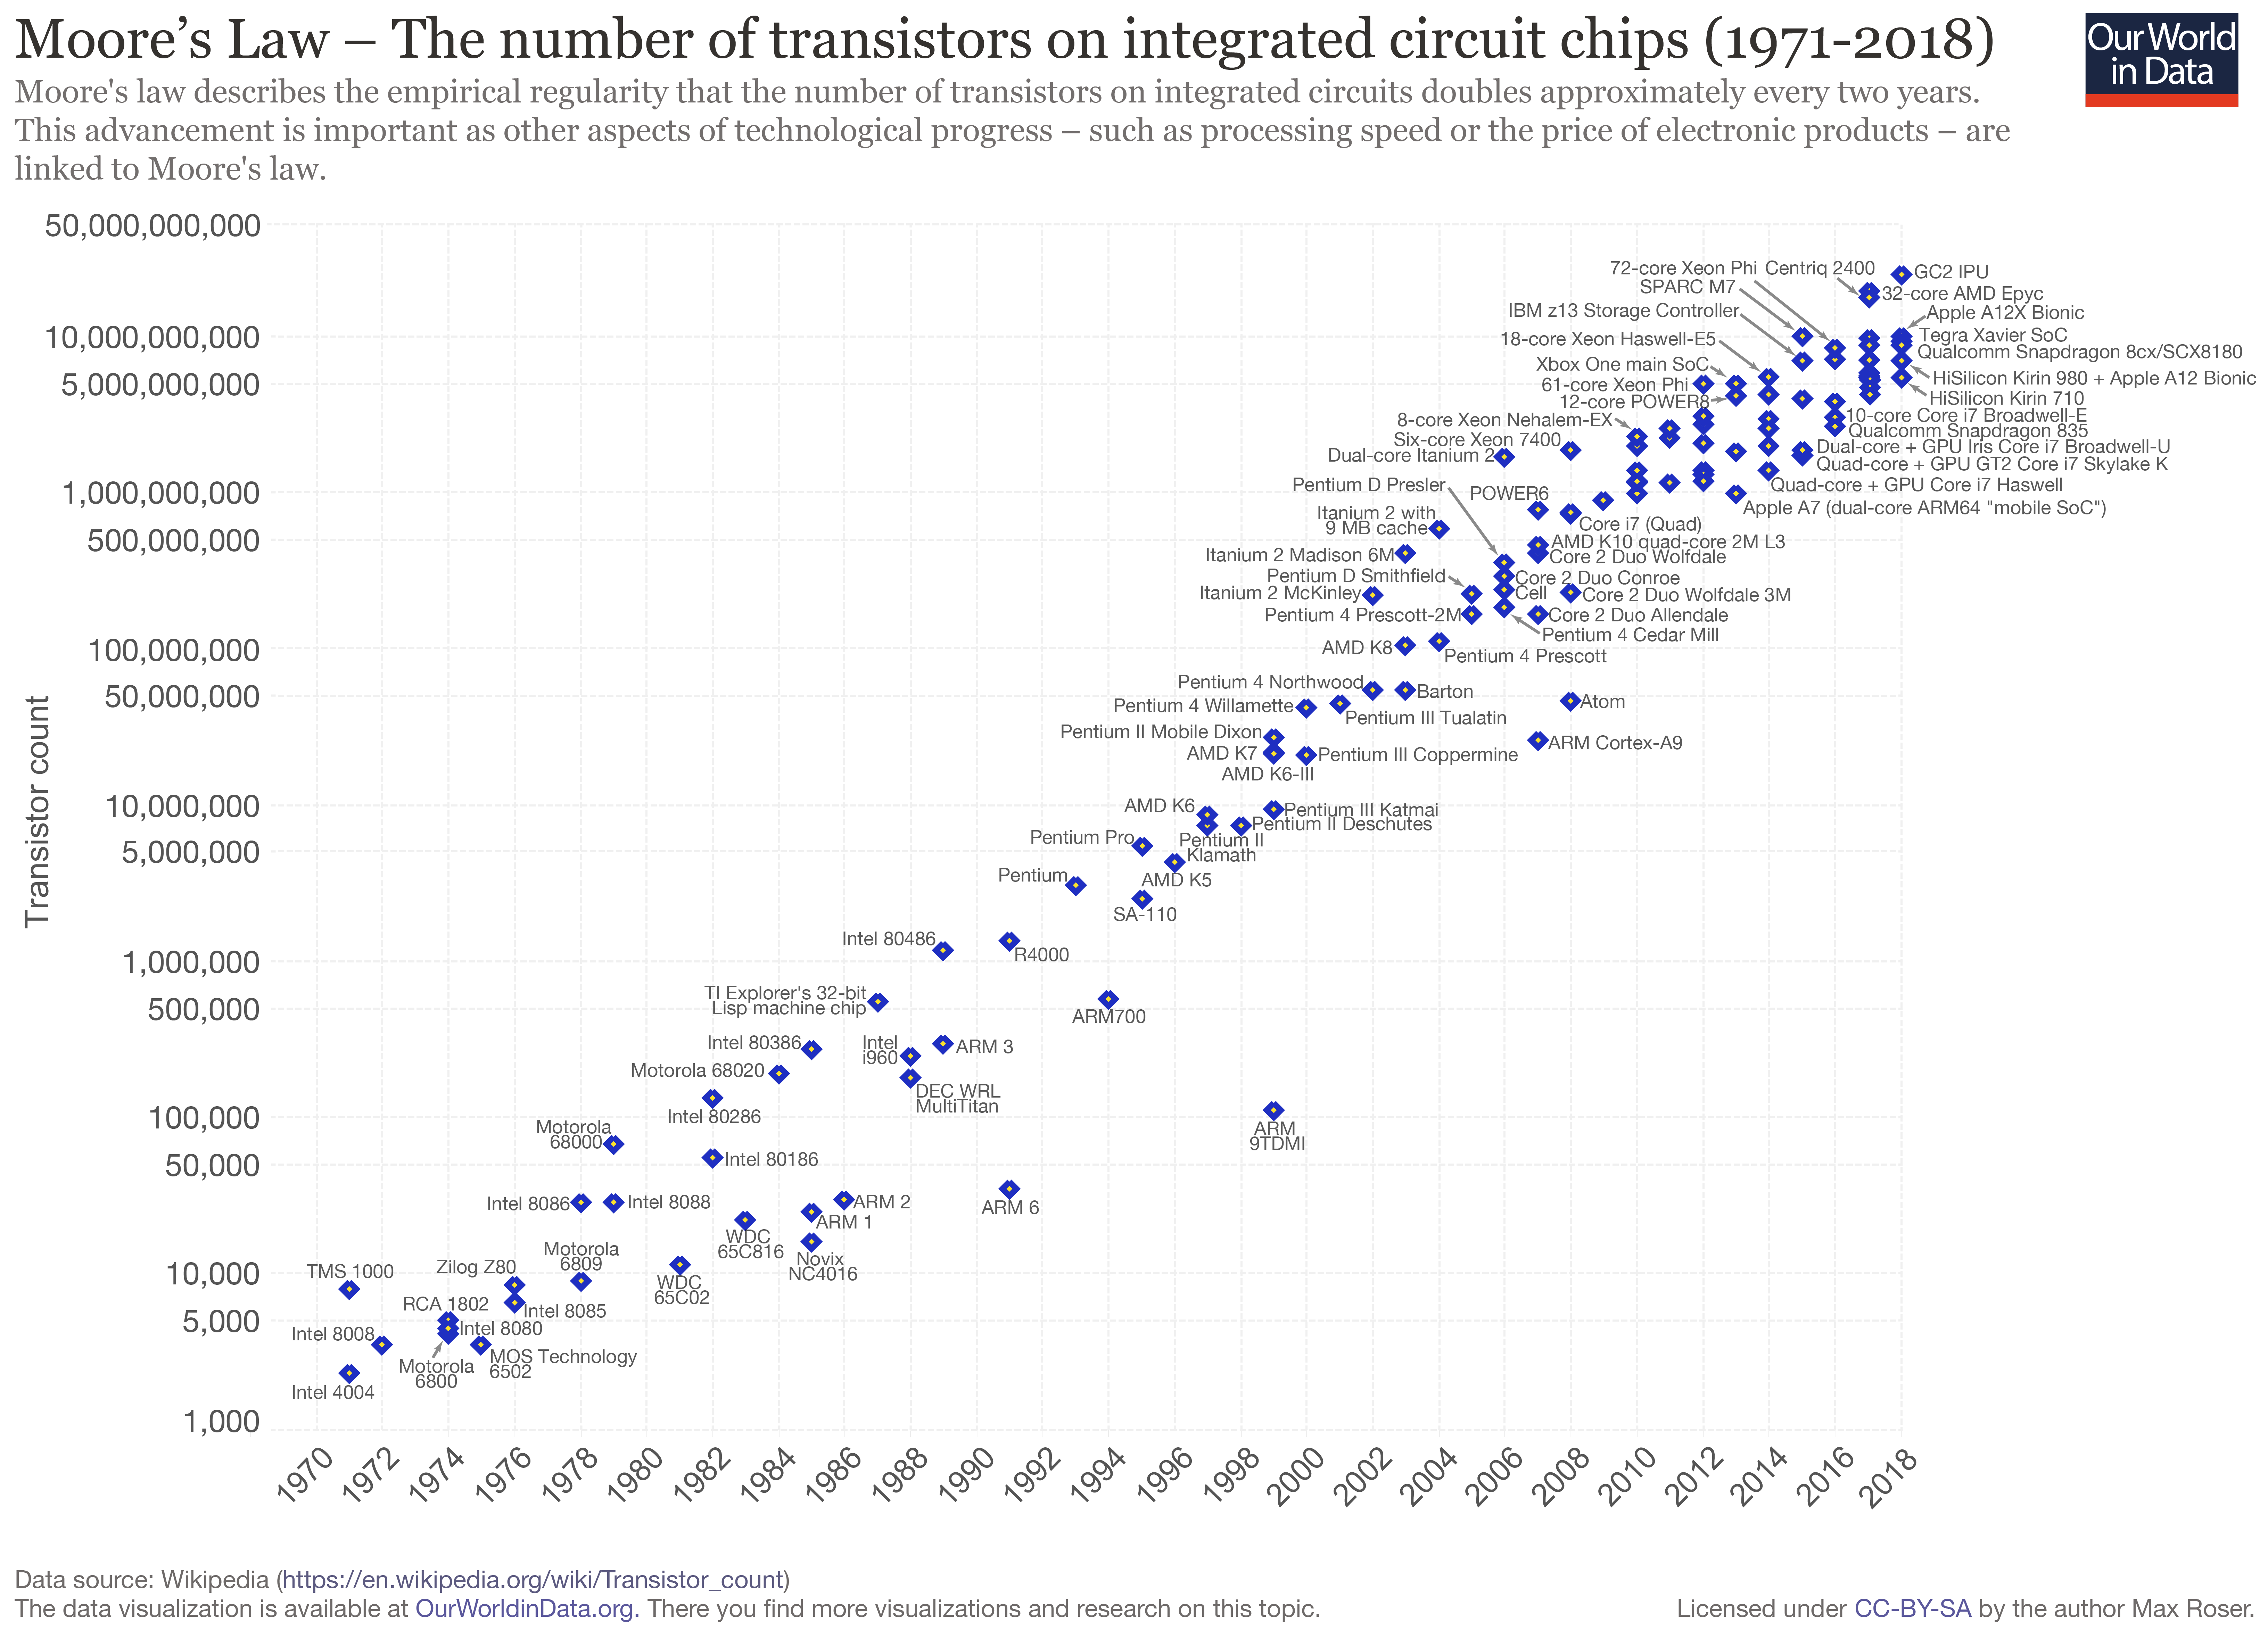
\includegraphics[width=10cm, height=7.5cm]{Bilder/Moore's_Law_Transistor_Count_1971-2018}  
%    \end{center}
%
\begin{figure}[h!]
	\centering
	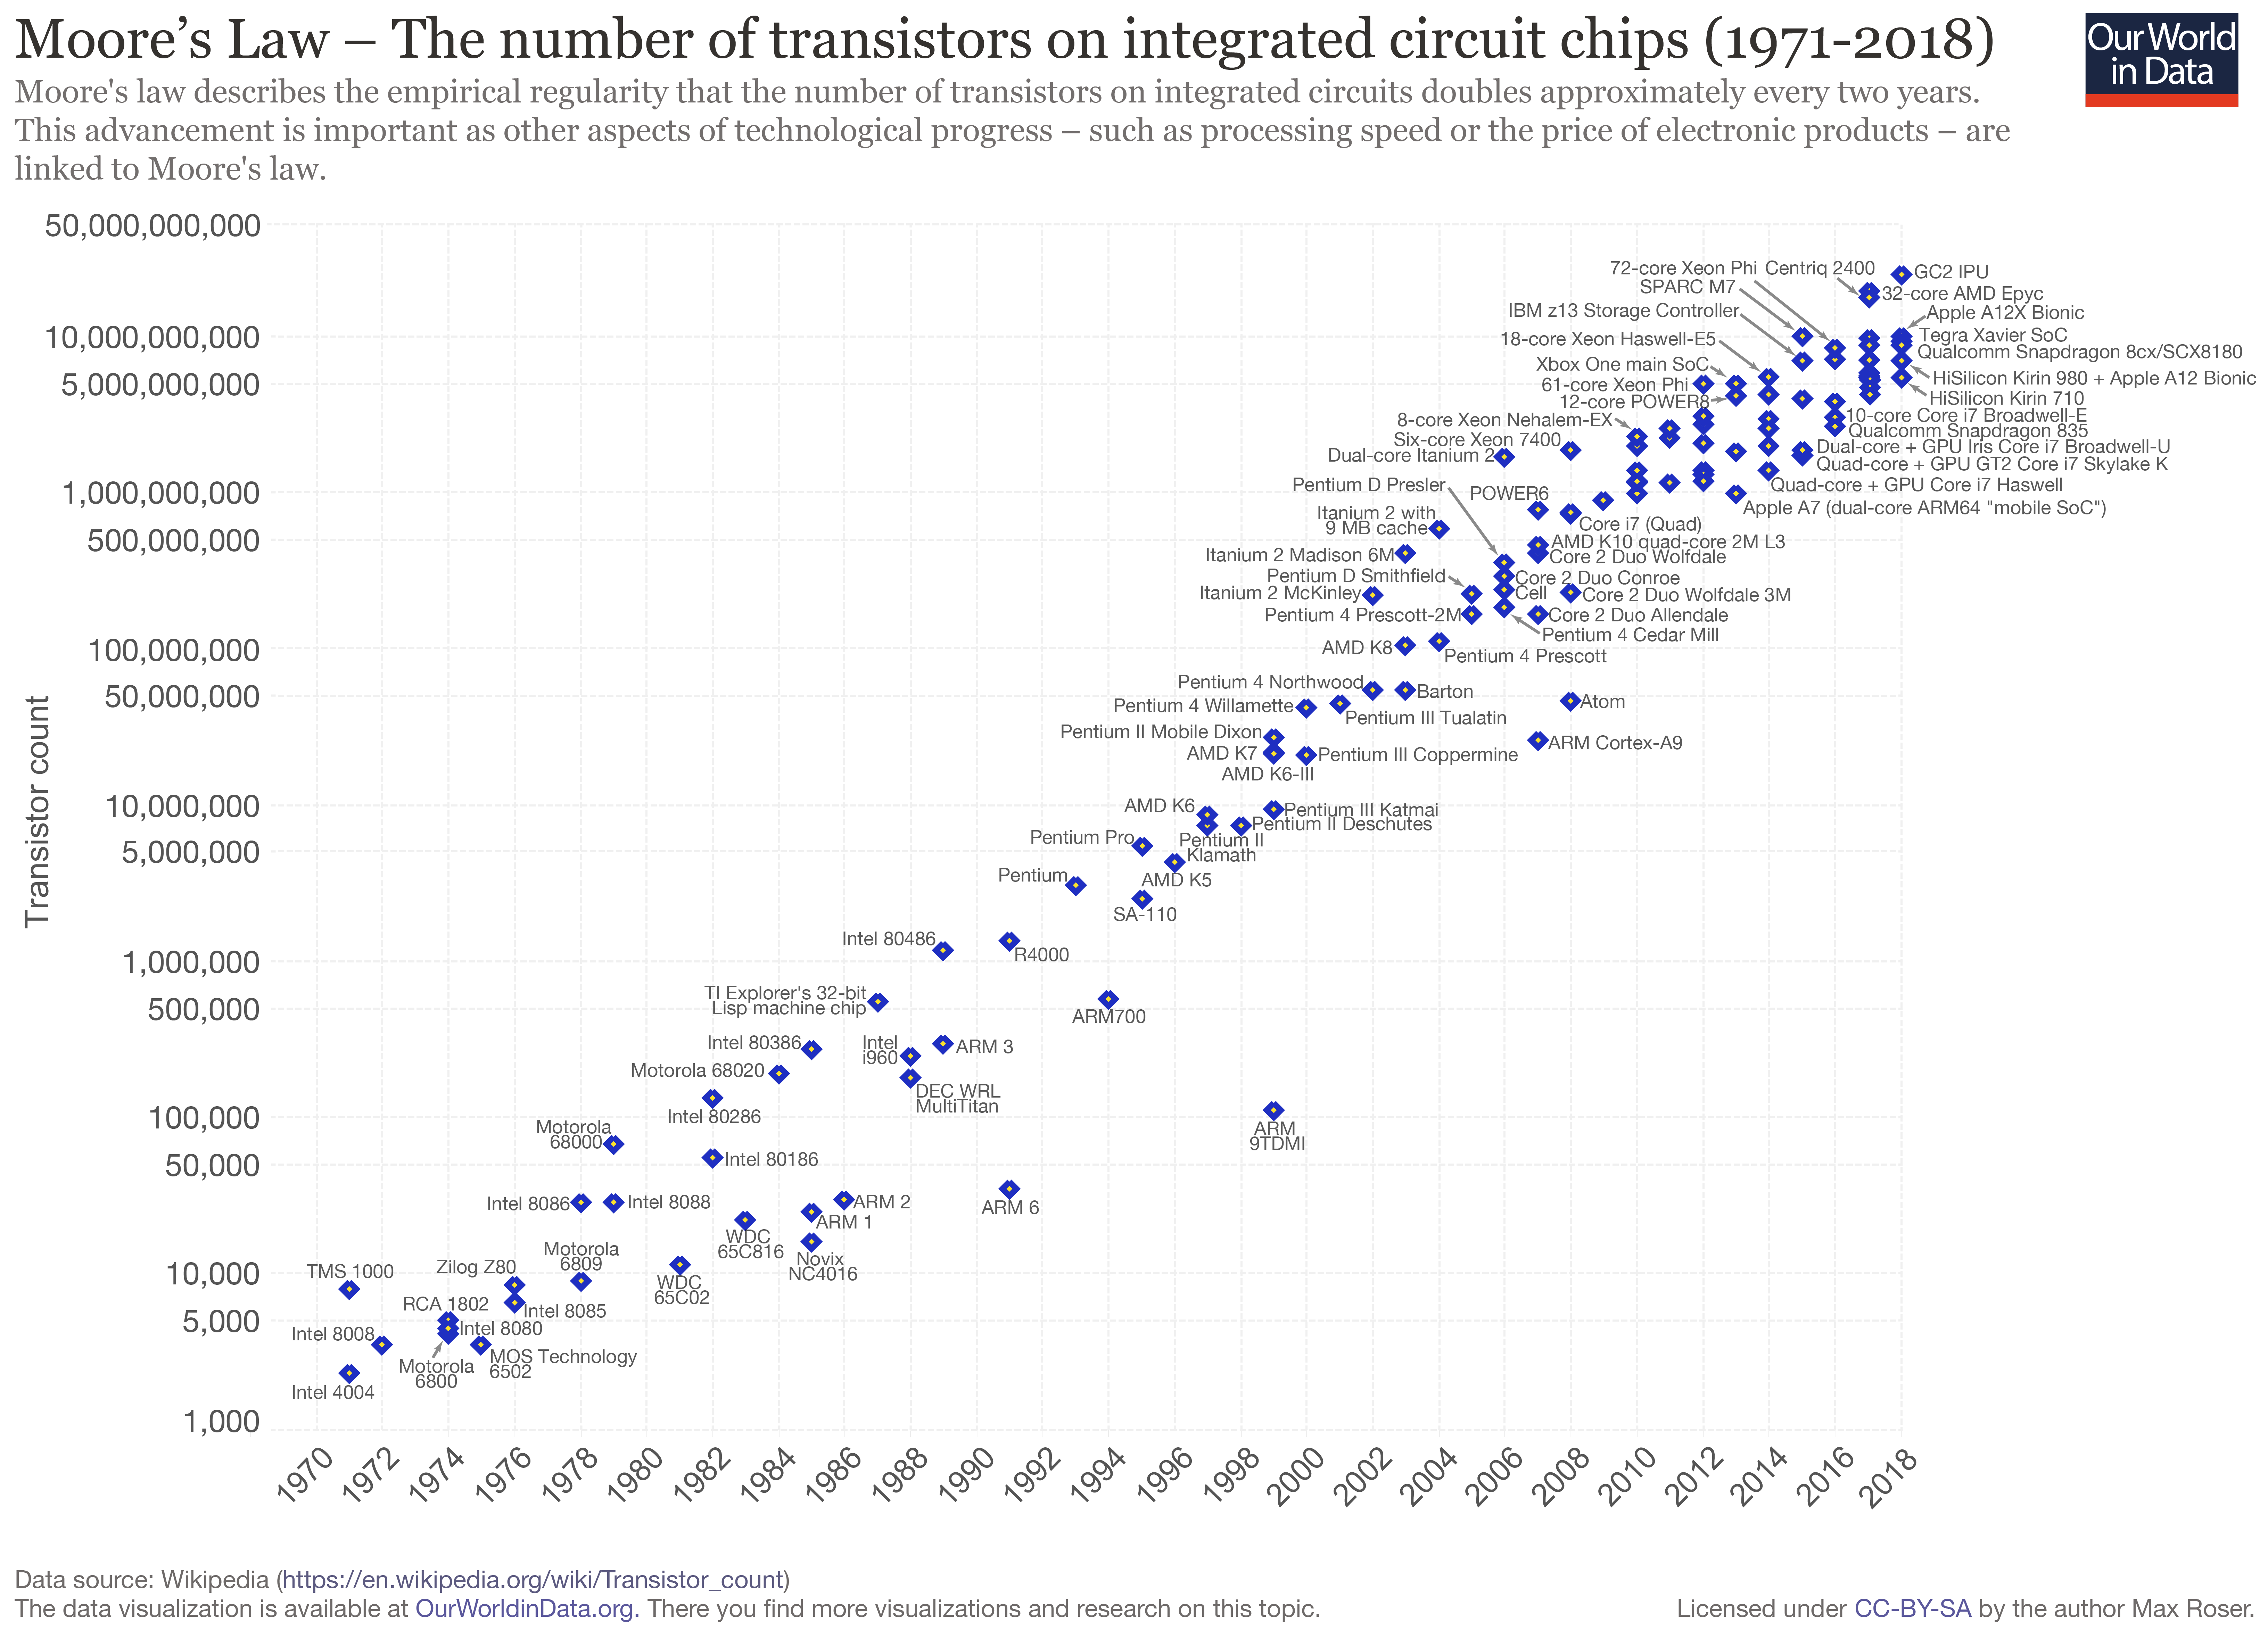
\includegraphics[width=12.5cm, height=8cm]{Bilder/Moore's_Law_Transistor_Count_1971-2018}		
	\caption{Mooresches Gesetz von 1971-2018} 
	\label{fig:moor}
\end{figure}
 
    
    \chapter{Grundlagen}\label{ch:Grundlagen} 
    \section{Matrix-Matrix Multiplikation}\label{sec:Matrix Multiplikation}
    Bei der Matrix-Matrix Multiplikation geht es um zwei Matrizen, die miteinander multipliziert werden. Aber nicht jede Matrizen sind miteinander multiplizierbar. D.h die Spaltenmatrix der ersten Matrix muss mit der Zeilenzahl der zweiten Matrix übereinstimmen. Das Ergebnis ist auch eine Matrix, die als Produktmatrix genannt wird.\\
    Gegeben seien zwei Matrizen.
    A ist eine  m$\times$n-Matrix.\\
    B ist eine  n$\times$p-Matrix.\\
    
   \textbf{ A}=$\begin{pmatrix}
    	a_{11} & a_{12} &  \ldots & a_{1n} \\
    	a_{21} & a_{22} &  \ldots & a_{2n} \\ 
    	\vdots & \vdots &  \ddots & \vdots \\
    	a_{m1} & a_{m2} &  \ldots & a_{mn} \\
    \end{pmatrix}$ , \textbf{B} = 
    $\begin{pmatrix}
    b_{11} & b_{12} &  \ldots & b_{1p} \\
    b_{21} & b_{22} &  \ldots & b_{2p} \\ 
    \vdots & \vdots &  \ddots & \vdots \\
    b_{n1} & b_{n2} &  \ldots & b_{np} \\
    \end{pmatrix}$\\
    
    Die Produktmatrix C ergibt sich:\\ \textbf{C} = 
    $\begin{pmatrix}
    c_{11} & c_{12} &  \ldots & c_{1p} \\
    c_{21} & c_{22} &  \ldots & c_{2p} \\ 
    \vdots & \vdots &  \ddots & \vdots \\
    c_{m1} & c_{m2} &  \ldots & c_{mp} \\
    \end{pmatrix}$\\
    
    Bei einer MM-Multiplikation finden $mpn$-Multiplikationen und $mp(n-1)$-Additionen statt.\\
    $c_{ij}=a_{i1}b_{1j}+a_{i2}b_{2j}+\ldots+a_{in}b_{nj}=\sum_{k-1}^{n} a_{ik}b_{kj}$\\
    
    
    \textbf{C}=$\begin{pmatrix}
    a_{11}b_{11}+ \ldots +a_{1n}b_{n1} & a_{11}b_{12}+\ldots +a_{1n}b_{n2} & \ldots & a_{11}b_{1p}+ \ldots +a_{1n}b_{np}  \\
    a_{21}b_{11}+ \ldots +a_{2n}b_{n1} & a_{21}b_{12}+\ldots +a_{2n}b_{n2} & \ldots & a_{21}b_{1p}+ \ldots +a_{2n}b_{np}  \\
    \vdots & \vdots &  \ddots & \vdots \\
    a_{m1}b_{11}+ \ldots +a_{mn}b_{n1} & a_{m1}b_{12}+\ldots +a_{mn}b_{n2} & \ldots & a_{m1}b_{1p}+ \ldots +a_{mn}b_{np}  
    \end{pmatrix}$\\
    
    
	
    
   
    \section{1D-Faltung und 2D-Faltung}\label{sec:Faltungsmatrix}
    
    \subsection{1D-Faltung bzw. Faltung}\label{subsec:1D-Faltung}
    Die Faltung mit eindimensionalen Signalen wird als 1D-Faltung oder nur Faltung bezeichnet. 1D-Faltung ist gut geeignet für Analyse einer Zeitreihe von Sensordaten oder von Signaldaten wie Tonaufnahme über einen Zeitraum fester Länge.  In der digitalen Bildverarbeitung und Signalverarbeitung findet meistens diskrete Faltung statt. Die Faltung von zwei diskreten Funktionen wird  durch folgende Formel berechnet:
    
    \begin{center}
    	$f[n]=a[n]\ast b[n] = \sum_{k=-\infty}^{\infty}a[k]  b[n-k]$
    \end{center}
	Die Faltung erfolgt durch Multiplizieren und Akkumulieren der Momentanwerte der überlappenden Abtastwerte. Dabei soll ein Signal umgedreht sein.
	
	
	

	\subsection{2D-Faltung}\label{subsec:2D-Faltung}
	Dieses Grundkonzept für 1D-Faltung gilt auch für die 2D-Faltung, wenn die Signale 2 Dimensionen haben. 	
	Analog kann die Faltung in 2D definiert werden.
	
	\begin{center}
		$f[x,y] = a[x,y]\ast b[x,y] = \sum_{j=-\infty}^{\infty}\sum_{k=-\infty}^{\infty} a[j,k] b[x-j , y-k]$
	\end{center}

%	 \begin{center}
%		$g\left( x,y\right) =\omega\ast f\left( x,y\right) = %\sum_{s=-a}^{a}\sum_{t=-b}^{b}\omega(s,t)f(x-s,y-t)$
%	\end{center}

	2D-Faltung ist ähnlich wie eine Matrix-Multiplikation und ziemlich eine einfache Operation. Hier wird ein Kernel gebraucht. Dieser Kernel ist eine Matrix von Gewichten und gleitet über die 2D-Eingangsmatrix. Dabei wird eine elementweise Multiplikation mit dem Teil der Eingabe durchgeführt, auf dem der Kernel sich befindet. siehe \autoref{fig:2DFaltung} Alle Ergebnisse nach der Multiplikation akkumuliert bzw. addiert  zu einem einzelnen Ausgabepixel.

	\subsubsection{Beispiel für 2D-Faltung}
	
	Hier ist ein Beispiel für 2D-Faltung. Es gibt ein 7x7 Eingangsmatrix I (inputmatrix) und eine Filtermatrix K (kernel) 3x3. Die Werte der Ausgangsmatrix werden durch Multiplikation und Addition von entsprechenden Pixelwerte von I und K berechnet. Siehe \autoref{fig:2DFaltung} 
	\newpage
	
\begin{figure}
	\centering
	%%%%%%%%%%%%%%%%%%%%%%%%%%%%%%%%%%%%%%%%%%%%%%%%%%%%%%%%%%%%%%%%%%%%%%%%%%%


%%%%%%%%%%%%%%%%%%% Local functions %%%%%%%%%%%%%%%%%%%
%% -- Draw marks
\newbox\dumbox
\newcommand{\mymark}[2]{%
	\setbox\dumbox=\hbox{#2}%
	\hbox to \wd\dumbox{\hss%
		\tikz[overlay,remember picture,baseline=(#1.base)]{ \node (#1) {\box\dumbox}; }%
		\hss}%
}

%% -- Draw small coefficient
\newcommand{\mysmall}[1]{%
	\tikz[overlay,remember picture]{%
		\node[blue,scale=.5, shift={(0,-.1)}] {x#1};%
	}%
}
%%%%%%%%%%%%%%%%%%% Local functions %%%%%%%%%%%%%%%%%%%



	\begin{center}

	
	
	\newcommand\numRowsK{3}
	\newcommand\numColsK{3}
	\newcommand{\K}[2]{% #1: row, #2: col
		\edef\Kcol##1##2##3{###2}%
		\edef\Krow##1##2##3{\noexpand\Kcol###1}%
		\Krow
		{1 0 1}
		{0 1 0}
		{1 0 1}%
	}
	
	\newcommand{\convoutionpicture}[2]{% #1: row to be highlighted, #2: colum to be highlighted
		\begin{tikzpicture}
		% ------- style -------
		\tikzset{%
			parenthesized/.style={%
				left delimiter  = (,
				right delimiter = ),
			},
			node distance = 10mu,
		}
		
		% ------- equation -------
		\matrix[matrix of math nodes, parenthesized, ampersand replacement=\&] (I) {
			0 \& 1 \& 1 \& 1 \& 0 \& 0 \& 0 \\
			0 \& 0 \& 1 \& 1 \& 1 \& 0 \& 0 \\
			0 \& 0 \& 0 \& 1 \& 1 \& 1 \& 0 \\
			0 \& 0 \& 0 \& 1 \& 1 \& 0 \& 0 \\
			0 \& 0 \& 1 \& 1 \& 0 \& 0 \& 0 \\
			0 \& 1 \& 1 \& 0 \& 0 \& 0 \& 0 \\
			1 \& 1 \& 0 \& 0 \& 0 \& 0 \& 0 \\
		};
		
		\node (*) [right = of I] {${}*{}$};
		
		\def\Kmatrix{}
		\foreach \row in {1, ..., 3} {
			\gdef \sep {}
			\foreach \col in {1, ..., 3} {%
				\xdef \Kmatrix {\unexpanded\expandafter{\Kmatrix}\unexpanded\expandafter{\sep}\noexpand \K{\row}{\col}}
				\gdef \sep { \& }
			}
			\xdef \Kmatrix {\unexpanded\expandafter{\Kmatrix}\noexpand\\}
		}
		\matrix[matrix of math nodes, parenthesized, ampersand replacement=\&] (K) [right = of *] {
			\Kmatrix
		};
		
		\node (=) [right = of K] {${}={}$};
		
		\matrix[matrix of math nodes, parenthesized, ampersand replacement=\&] (I*K) [right = of {=}] {
			1 \& 4 \& 3 \& 4 \& 1 \\
			1 \& 2 \& 4 \& 3 \& 3 \\
			1 \& 2 \& 3 \& 4 \& 1 \\
			1 \& 3 \& 3 \& 1 \& 1 \\
			3 \& 3 \& 1 \& 1 \& 0 \\
		};
		
		% ------- highlighting -------
		\def\rowResult{#1}
		\def\colResult{#2}
		
		\begin{scope}[on background layer]
		\newcommand{\padding}{2pt}
		\coordinate (Is-nw) at ([xshift=-\padding, yshift=+\padding] I-\rowResult-\colResult.north west);
		\coordinate (Is-se) at ([xshift=+\padding, yshift=-\padding] I-\the\numexpr\rowResult+\numRowsK-1\relax-\the\numexpr\colResult+\numColsK-1\relax.south east);
		\coordinate (Is-sw) at (Is-nw |- Is-se);
		\coordinate (Is-ne) at (Is-se |- Is-nw);
		
		\filldraw[red,   fill opacity=.1] (Is-nw) rectangle (Is-se);
		\filldraw[green, fill opacity=.1] (I*K-\rowResult-\colResult.north west) rectangle (I*K-\rowResult-\colResult.south east);
		
		\draw[blue, dotted] 
		(Is-nw) -- (K.north west)
		(Is-se) -- (K.south east)
		(Is-sw) -- (K.south west)
		(Is-ne) -- (K.north east)
		;
		\draw[green, dotted] 
		(I*K-\rowResult-\colResult.north west) -- (K.north west)
		(I*K-\rowResult-\colResult.south east) -- (K.south east)
		(I*K-\rowResult-\colResult.south west) -- (K.south west)
		(I*K-\rowResult-\colResult.north east) -- (K.north east)
		;
		
		\draw[blue,  fill=blue!10!white] (K.north west) rectangle (K.south east);
		
		\foreach \row [evaluate=\row as \rowI using int(\row+\rowResult-1)] in {1, ..., \numRowsK} {%
			\foreach \col [evaluate=\col as \colI using int(\col+\colResult-1)] in {1, ..., \numColsK} {%
				\node[text=blue] at (I-\rowI-\colI.south east) [xshift=-.3em] {\tiny$\times \K{\row}{\col}$};
			}
		}
		\end{scope}
		
		% ------- labels -------
		\tikzset{node distance=0em}
		\node[below=of I] (I-label) {$I$};
		\node at (K |- I-label)     {$K$};
		\node at (I*K |- I-label)   {$I*K$};
		\end{tikzpicture}
	}
	
%	\begin{document}
		\convoutionpicture 14
		\bigskip
		
		\convoutionpicture 41
		\bigskip
		
		\convoutionpicture 55
	%\end{document}
	\end{center}
%%%%%%%%%%%%%%%%%%%%%%%%%%%%%%%%%%%%%%%%%%%%%%%%%%%%%%%%%%%%%%%%%%%%%%%%%%%
	\caption{Visualisierung von 2D Faltung}
	\label{fig:2DFaltung}
\end{figure}
	%\cleardoublepage
	
%%%%%%%%%%%%%%%%%%%%%%%%%%%%%%%%%%%%%%%%%%%%%%%%%%%%%%%%%%%%%%%%%%%%%%%%%%%%%%%%%%%%%%%%%%%%%%%%%


%%%%%%%%%%%%%%%%%%%%%%%%%%%%%%%%%%%%%%%%%%%%%%%%%%%%%%%%%%%%%%%%%%%%%%%%%%%%%%%%%
				

	\section{Maschinelles Lernen}\label{sec:Maschinelles Lernen}
	Beim ML wird das System so programmiert, damit das aus eingegebenen Daten automatisch lernt und sich mit der \grqq Erfahrung\grqq  verbessert. Das heißt, das System wird mit Trainingsdaten trainiert. Hier bedeutet das Lernen: die eingegebenen Daten zu erkennen, verstehen und auf der Grundlage der gelieferten Daten eine sinnvolle Entscheidung zu treffen.
	Aber nicht alle Entscheidungen können auf der Grundlage aller möglichen Eingaben berücksichtigt werden. Um dieses Problem  zu lösen, werden hier Algorithmen 	entwickelt, die das maschinelles Lernen optimieren und schneller machen.

	
	\section{Lernphase}\label{sec:Lernphase}
	\subsection{Supervised Learning}\label{subsec:Supervised Learning}
	Beim supervised Learning brauchen die Trainingsdaten Label (Lösungen).
	D.h. man muss als Entwickler dem Modell vorher sagen, was die Lösung ist.
	Wenn man beispielsweise einem Bildererkenner beibringen will, Hunde-und Katzenbilder 
	zu unterscheiden, muss vorher ein Mensch alle Trainingsbilder anschauen und notieren 
	was zu sehen ist. Hier ist der Entwickler als ''Lehrer'' vorgesehen, der das ML-Modell beibringt. Ansonsten weiss der Algorithmus nicht, ob er falsch oder richtig entscheidet.\\
	\textbf{Anwendungen}
	\begin{description}
		\item[Bildklasifizierung] In der Zukunft wird von dem System erwartet, dass es ein neu gegebenes Bild erkennt.
		\item[Marktvorhersage] Das System wird von Werten aus der vergangenen Marktdaten trainiert und wird erwartet, dass es den Preis für die Zukunft vorhersagt.
		\begin{center}
			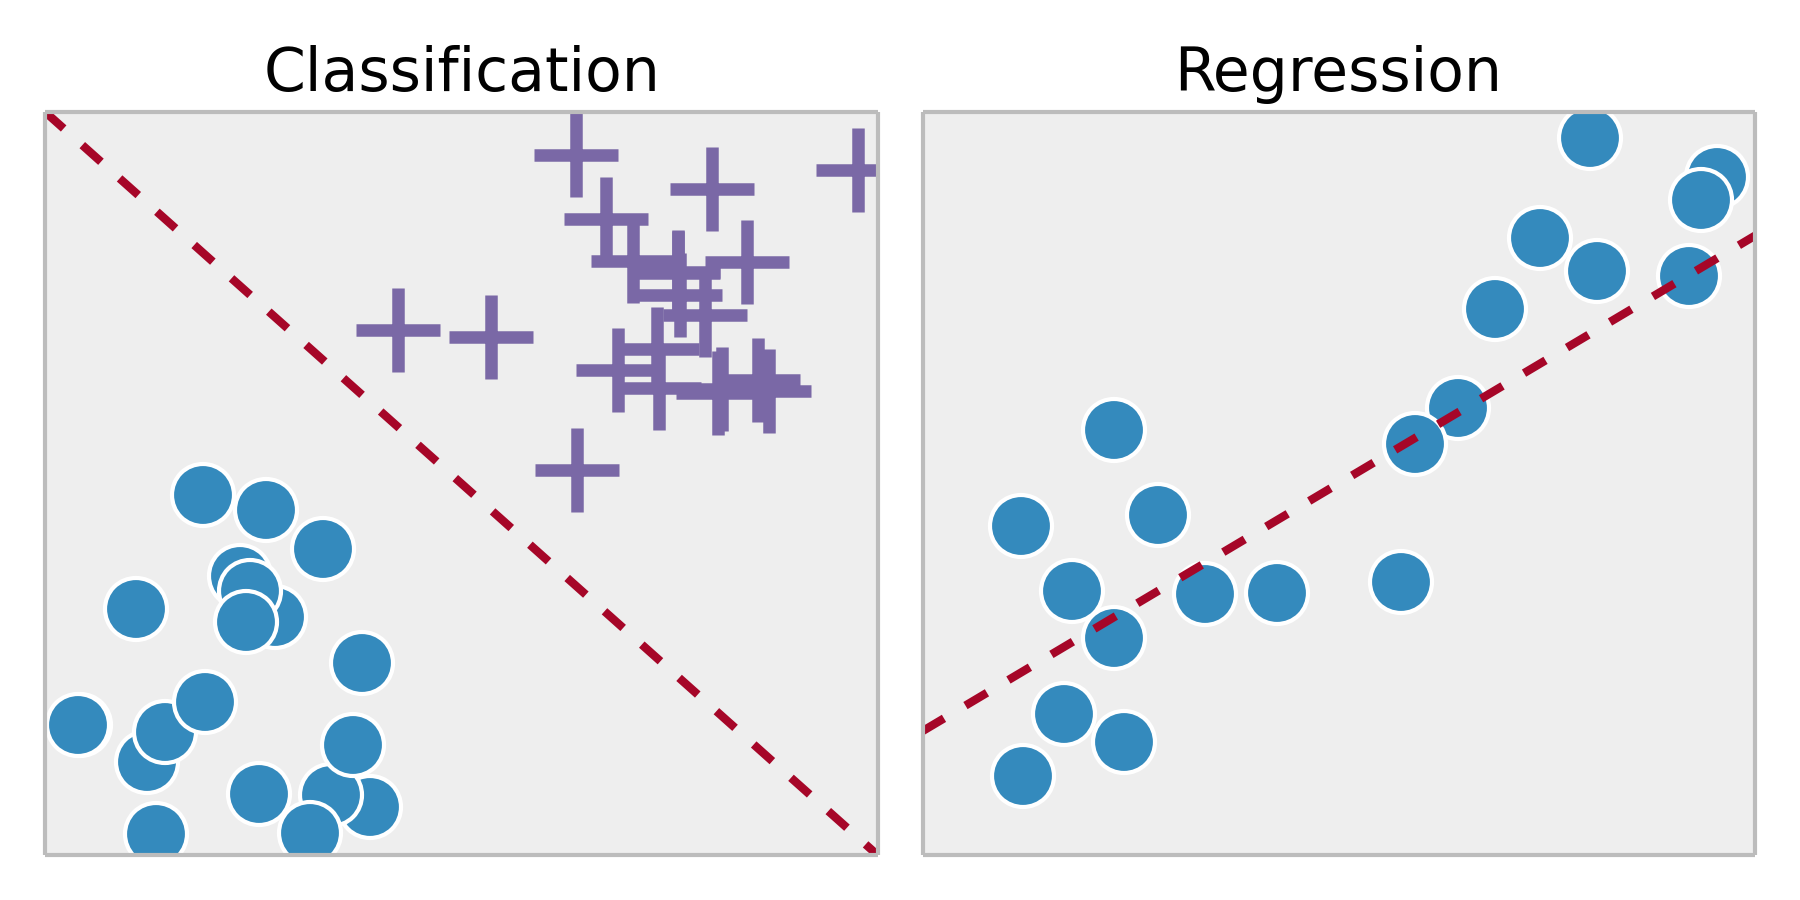
\includegraphics[width=15 cm , height= 7 cm]{Bilder/clasreg}
		\end{center}  
	\end{description}
	
	

	\subsection{Unsupervised Learning}\label{subsec:Unsupervised Learning}
	Beim Unsupervised Learning soll das ML-Modell aus Daten ''lernen'', die Bedeutungen von denen noch unbekannt sind. Hier wird dem Algorithmus die Daten ohne Zielvorgabe eingespeist und trainiert. Ohne Daten gibt es natürlich nichts zu ''lernen''.
	Unsupervised Learning wird verwendet, um einen bestimmten Datensatz in verschiedene Gruppen zu gruppieren. Dies wird häufig verwendet, um Kunden für bestimmte Eingriffe in verschiedene Gruppen zu segmentieren.\\
	%\newpage
	\textbf{Anwendungen}
	\begin{description}
		\item[Clustering] Ähnliche Daten werden in Cluster bzw. Gruppen eingeteilt, um die Gruppierung für ein Zweck zu nutzen. Dies ist in Forschung und Wissenschaft eingesetzt. 
		\begin{center}
			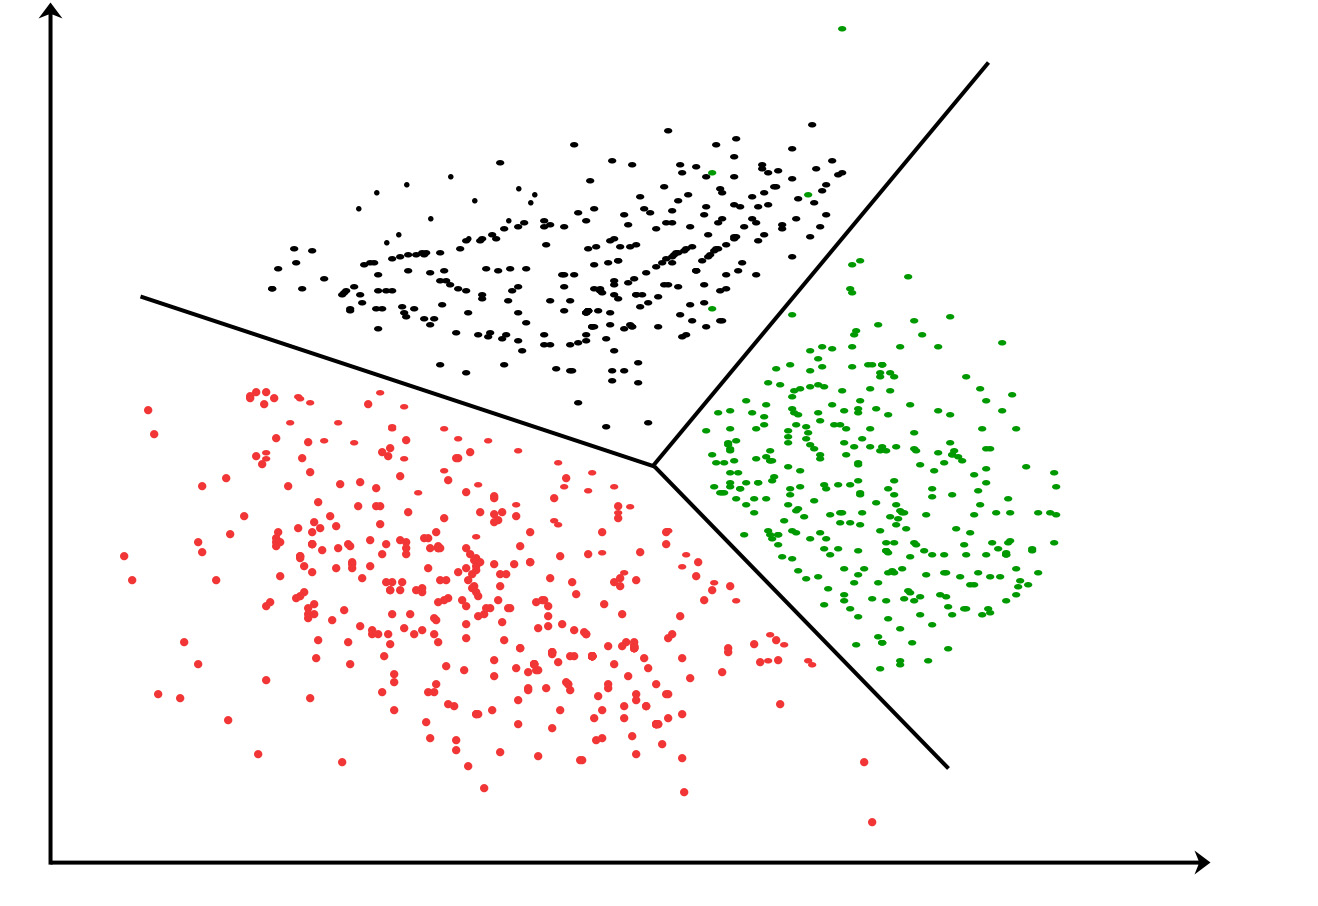
\includegraphics[width=15 cm , height= 7 cm]{Bilder/clustering}
		\end{center}  
	\end{description}
	


	\subsection{Reinforcement Learning}\label{subsec:Reinforcement Learning}
	Bei der reinforcement Learning geht es darum, dass der Agent (hier: Software-Bot) in einer unbekannten und komplexen Umgebung sein Ziel erreicht. Dabei wird der Agent für richtiges Aktion belohnt und für falsches Aktion bestraft. Sein Ziel ist es, die Gesamtbelohnung zu maximieren bzw. Strafen zu minimieren. Der Unterschied zwischen Supervised-und Reinforcement Learning ist es, dass der Agent keine Hinweise oder Vorschläge zur Lösung bekommt. Die Lösung ist unbekannt und er versteht nur aus seiner Aktion, ob er falsch oder richtig liegt. 
	%\newpage
	
		\section{Kuenstliche neuronale Netze} \label{sec:Kuenstliche neuronale Netze}
	Kuenstliche neuronale Netze sind ein Technik des ML, die den Mechanismus des Lernens in biologischen Organismen simulieren. \cite{haykin1994neural} Das menschliche Nervensystem enthält Zellen, die als Neuron bezeichnet wird.  Jedes Neuron besteht aus drei Teile: Es sind die Dendriten, der Zellkörper und das Axon. \autoref{fig:neuron} Aus dem Zellkörper verzweigen sich eine Reihe von Fasern ab, die Dendritte genannt werden. Die Lange Faser wird Axon genannt und streckt sich nach große Entfernungen. Es kann von 1cm bis 1 Meter lang sein.\\
	Ein Neuron kann mit anderen Neuronen 10 bis 100.000 Verbindungen herstellen, die als Synapsen bezeichnet werden. Die Kommunikationen zwischen Neuronen erfolgen mit elektrochemischen Signalen.  
	
	
	
	
	%	 elektrochemische Signale von anderen Neuronen zum Zellkörper übertragen.  Das Axon erstreckt sich über eine lange Strecke, um das Signal von einem Neuron zu einem Anderen zu übertragen.
	
	%	\begin{center}
	%		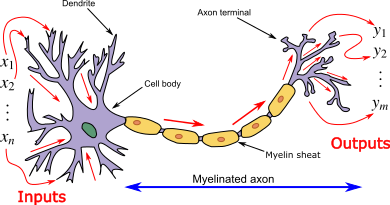
\includegraphics[width=10 cm , height= 5 cm]{Bilder/neuron}
	%	\end{center}
	
	\begin{figure}
		\centering
		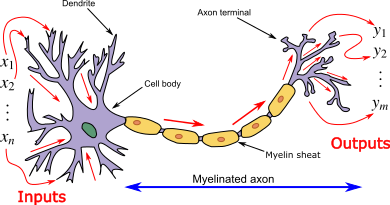
\includegraphics[width=10 cm , height= 5 cm]{Bilder/neuron}
		\caption{Aufbau eines Neurons}
		\label{fig:neuron}
	\end{figure}
	
	
	
	Dieser biologische Mechanismus wird in kuenstlichen neuronalen Netzen übertragen. Ein Neuron ist eine Einheit für die Informationsverarbeitung, das sich die Grundlage einer neuronaler Netze bildet.
	
	%hier kommt neuron
	\begin{figure}
		\centering
		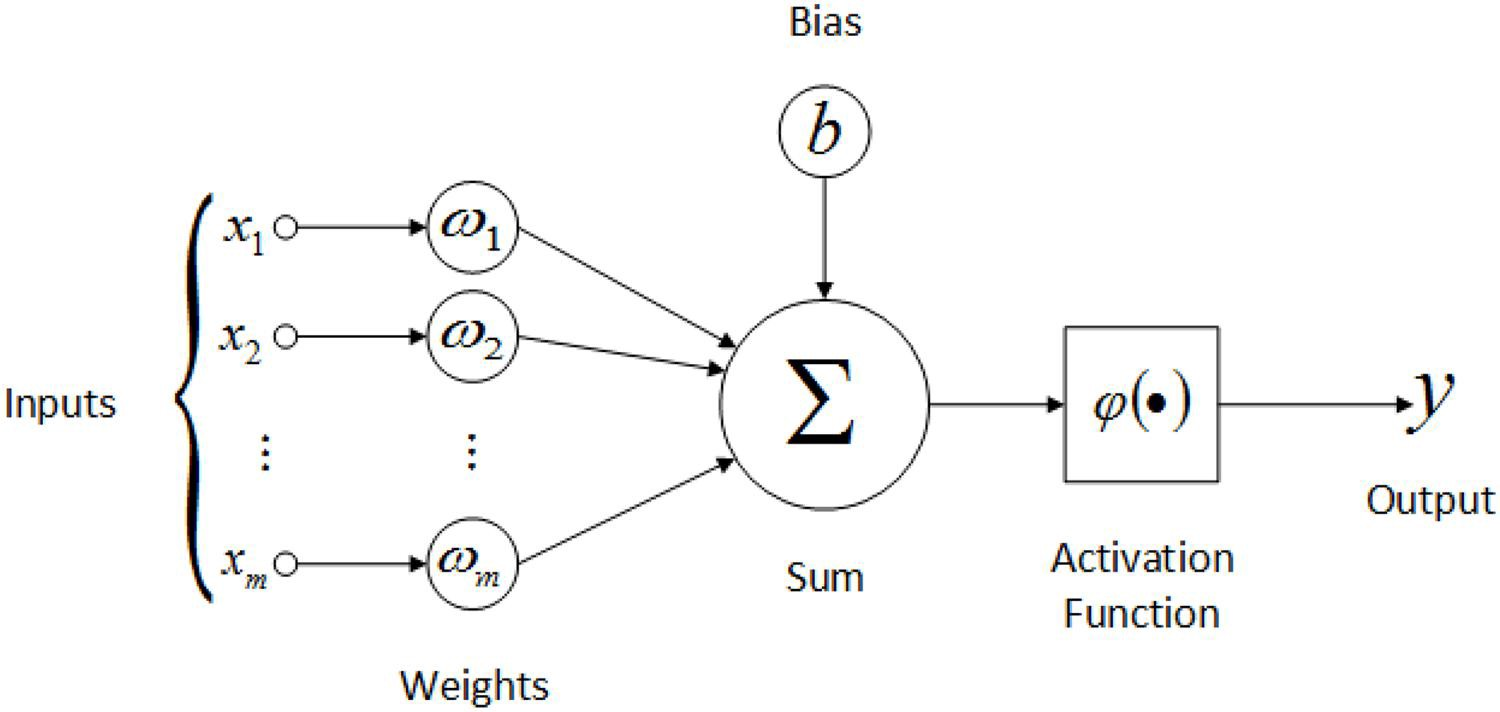
\includegraphics[width=10 cm , height= 5 cm]{Bilder/artneuron}
		\caption[Künstliches Neuron]{Die Eingänge $x_{1},x_{2}, \ldots , x_{m}$ sind mit Gewichten $w_{1},w_{2}, \ldots , w_{m}$ multipliziert und diese Werte werden durch Übertragungsfunktion summiert und Bias hinzugefügt. Die Aktivierungsfunktion hat dann den Ausgangswert bestimmt.}
		\label{fig:artneuron}
	\end{figure}
	
	
	\begin{description}
		\item[\textbf{Gewichtung $w_{i}$ :}] Sie bestimmen den Grad, wie stark die Eingänge der Entscheidung des Neurons beeinflusst. Ein Gewicht mit dem Wert 0 bedeutet, dass es keine Verbindung zwischen Neuronen existiert.
		\item[\textbf{Übertragungsfunktion:}] Die Netzeingabe wird durch die Übertragungsfunktion $\sum$ von einzelnen Einganswerte, die mit Gewichte multipliziert sind, berechnet.
		
		\item[\textbf{Bias}]: Die Übertragungsfunktion enthält noch ein externer Wert, die mit Bias $b$ bezeichnet ist. Das kann auch positive und negative Werte einnehmen und hat Einfluss auf den Eingangswert der Aktivierungsfunktion. Damit wird dieser Wert erhöht oder auch gesenkt werden.
		
		
		\item[\textbf{Aktivierungsfunktionen:}]
		%{Aktivierungsfunktionen}\label{subsec:Aktivierungsfunktionen}
		Eine Aktivierungsfunktion ist eine mathematische Funktion und entscheidet, ob ein Neuron aktiviert werden soll oder nicht, indem sie die gewichtete Summe berechnet und eine Bias hinzufügt. Diese Funktionen sind:	
		
		\subsection{Schwellenwertfunktion}\label{subsec:Schwellenwertfunktion}
		Die Schwellenwertfunktion (engl. heaviside step function oder auch binary step function) nimmt nur die Werte 0 und 1 an. Liegt der Eingabewert über oder unter einem bestimmten Schwellenwert, wird das Neuron aktiviert und sendet das Eingangssignal. Für die Eingabe e$\geq$ {0} nimmt der Ausgangswert 1, ansonsten 0.\\
		
		
		%%%%%%%%%%%%%%%%%%%%%%%%%%%%%%%%%%%%%%%%%%%
		
		\begin{minipage}{.5\linewidth}
			\begin{eqnarray*}
				\varphi (e) = 
				\begin{cases}
					0 & \text{wenn $e<0$} \\
					1 & \text{wenn $e\geq0$} \\
				\end{cases}
			\end{eqnarray*}
		\end{minipage}
		\begin{minipage}{.5\linewidth}
			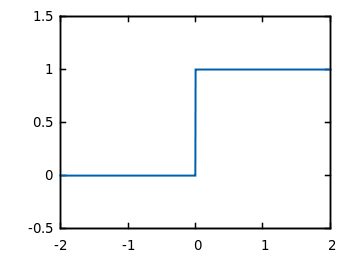
\includegraphics[width=5 cm , height= 5 cm]{Bilder/step}
			%				
		\end{minipage}
		
		
		
		
		
		%%%%%%%%%%%%%%%%%%%%%%%%%%%%%%%%%%%%%%%%%%%	
		
		
		
		
		
		
		\subsection{Stückweise lineare Funktion}
		Stückweise lineare Funktion  läuft in einem begrenzten Intervall linear ab. Außerhalb des Intervalls besitzt die Funktion einen konstanten Wert.\\
		%$\varphi (e) = 
		%	\begin{cases}
		%	0 & \text{wenn $e\leq -\dfrac{1}{2}$} \\
		%	1 & \text{wenn $e\geq \dfrac{1}{2}$} \\
		%	e + 1/2 & \text{wenn  $-\dfrac{1}{2} < e < \dfrac{1}{2} $ }
		%\end{cases}$\\
		
		
		
		\begin{minipage}{.5\linewidth}
			\begin{eqnarray*}
				\varphi (e) = 
				\begin{cases}
					0 & \text{wenn $e\leq -\dfrac{1}{2}$} \\
					e + 1/2 & \text{wenn  $-\dfrac{1}{2} < e < \dfrac{1}{2} $ }\\
					1 & \text{wenn $e\geq \dfrac{1}{2}$} 
					
				\end{cases}
			\end{eqnarray*}
		\end{minipage}
		\begin{minipage}{.5\linewidth}
			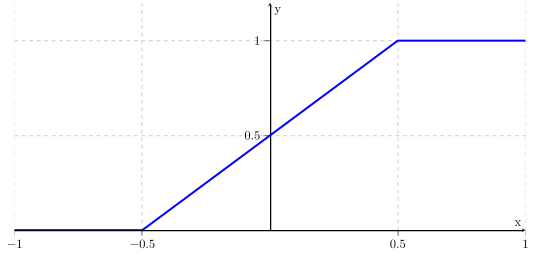
\includegraphics[width=7 cm , height= 5 cm]{Bilder/stf}
			
		\end{minipage}
		%				
		\newpage
		
		\subsection{Sigmoidfunktion}
		Sigmoide Funktionen sind sehr häufig verwendete Funktionen. Sie besitzen ein variables Steigungsmaß $\alpha $ , dass die Krümmung des Funktionsgraphen beeinflusst. Differenzierbarkeit der Sigmoidfunktion ist für einige ML-Verfahren wie Backpropagation-Algorithmus ein Vorteil. Der Nachteil ist ein starker negativer Eingangssignal, damit kann es während des Trainings hängen bleiben.\\Sie ist definiert durch: 
		
		
		
		
		
		
		%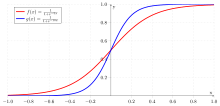
\includegraphics[width=7 cm , height= 5 cm]{Bilder/sigmoid}
		\begin{tikzpicture}
		\begin{axis}[legend pos=north west,
		axis x line=middle,
		axis y line=middle,
		x tick label style={/pgf/number format/fixed,
			/pgf/number format/fixed zerofill,
			/pgf/number format/precision=1},
		y tick label style={/pgf/number format/fixed,
			/pgf/number format/fixed zerofill,
			/pgf/number format/precision=1},
		grid = major,
		width=16cm,
		height=8cm,
		grid style={dashed, gray!30},
		xmin=-1,     % start the diagram at this x-coordinate
		xmax= 1,    % end   the diagram at this x-coordinate
		ymin= 0,     % start the diagram at this y-coordinate
		ymax= 1,   % end   the diagram at this y-coordinate
		%axis background/.style={fill=white},
		xlabel=x,
		ylabel=y,
		tick align=outside,
		enlargelimits=false]
		% plot the stirling-formulae
		$\addplot[domain=-1:1, red, ultra thick,samples=500] {1/(1+exp(-5*x))};$
		$\addplot[domain=-1:1, blue, ultra thick,samples=500] {1/(1+exp(-10*x))};$
		$\addlegendentry{$f(x)=\frac{1}{1+e^{-5x}}$}$
		$\addlegendentry{$g(x)=\frac{1}{1+e^{-10x}}$}$
		\end{axis}
		
		\end{tikzpicture}
		
		\begin{center}
			$\varphi_{\alpha}^{sig} (e) = \dfrac{1}{1+\exp (-\alpha e)}$
		\end{center}
		
		\subsection{Rectifier (ReLU)}
		Es wird besonders in Deep-Learning Modellen wie CNN( Convolutional Neural Networks) eingesetzt. Dies ist auch als Rampenfunktion bekannt. ReLU Funktion ist definiert durch:
		
		
		\begin{minipage}{.5\linewidth}
			\begin{eqnarray*}
				\varphi (e) = \max (0,e)
			\end{eqnarray*}
		\end{minipage}
		\begin{minipage}{.5\linewidth}
			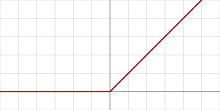
\includegraphics[width=7 cm , height= 5 cm]{Bilder/ReLu}
		\end{minipage}
	\end{description}
	
	
	\newpage
	
	
	\textbf{Kurze Zusammenfassung:} Ein Neuron \autoref{fig:simple_neuron} besitzt viele Eingaben und jede Eingabe des Neurons wird mit einem Gewicht versehen. Die gewichteten Eingaben werden dann durch eine Übertragungsfunktion akkumuliert und daraus resultierende Netzeingabe in eine Aktivierungsfunktion gegeben, die die Ausgabe $a_{j} = g(\sum_{i=0}^{n} w_{m,j}a_{i})$ bestimmt.
	
	
	\begin{figure}[h!]
		\centering
		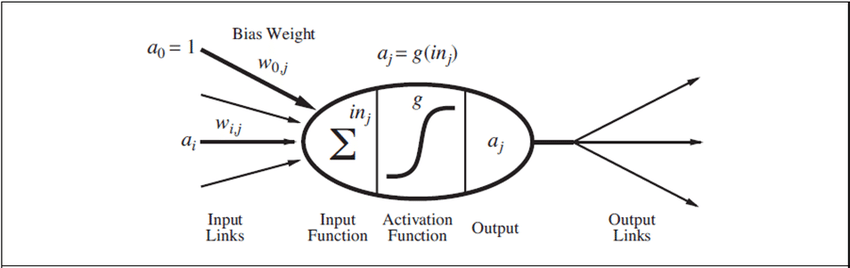
\includegraphics[width=16.5 cm , height= 5 cm]{Bilder/simple_neuron}
		\caption{Ein vereinfachtes mathematisches Modell für ein künstliches Neuron}
		\label{fig:simple_neuron}	
			
	\end{figure}

	\section{Strukturen der kuenstlichen neuronalen Netzwerke}\label{sec:Strukturen der kuenstlichen neuronalen Netzwerke}
	Modelle der künstlichen neuronalen Netzwerke können als eine Reihe von grundlegenden Verarbeitungseinheiten verstanden werden, die miteinander eng verbunden sind. Das Ziel ist, die eingegebenen Daten ins neuronale Netz so verarbeiten, um gewüschten Ausgaben zu erzeugen.\\
	In diesem Abschnitt wird die grundlegende Architektur von neuronalen Netzwerken diskutiert. Es gibt einschichtiges- \textbf{(single-layer)} und mehrschichtiges \textbf{(multi-layer)} neuronales Netz. In einem einschichtigen Netz wird der Ausgang direkt über die Aktivierungsfunktion mit den Eingängen verbunden. Dies wird in der Fachsprache auch als Perzeptron genannt. Das mehrschichtige Netz besteht aus Eingangs- und Ausgangsschicht\\ engl. \textbf{(input- and output layers)} und zwischen diesen Schichten befinden sich die versteckte Schichten engl. \textbf{(hidden-layer)}. 
	Die Informationen, die im neuronalen Netz verbreiten, können in zwei Kategorien eingeteilt werden. 
	
	\begin{description}
		\item[feedforward-Netze] Der Informationsfluss in einem feedforward-Netz erfolgt nur in eine Richtung. Wenn man das Netz als Graph und Neuronen als Knoten betrachtet, dann das Graph darf keine Schleifen oder Zyklen enthalten. Mehrschichtiges Netz und convolutional neural Network (CNN) sind gute Beispiele für feedforward-Netze. \cite{AGuidetoConvolutional}
		\newpage
		\item[feedback-Netze] Die feedback-Netze können Zyklen oder auch Schleifen enthalten. Die Auszeichnung des feedback-Netzes ist die Errinerungsfähigkeit und kann Informationen und Daten speichern. Beiscpiele für solche Architekturen sind Recurrent neural Network und Long-Short-Term-Memory (LSTM). 
 	\end{description}
	
	
	
%	Diese schichtweise Architektur des neuronalen Netzwerk wird auch als feedforward Netzwerk bezeichnet. 
	
	
%	Zuerst wird die single-layer neuronale Netzwerk vorgestellt, die auch in der Literatur Perceptron genannt wird.
	
	\subsection{Einlagiges Perzeptron}

	\begin{minipage}[t]{.6\textwidth}%
		Ein einlagiges Perzeptron enthält eine einzelne Eingabeebene und einen Ausgabeknoten. Die Eingabewerte $x_{1},x_{2},x_{3}, \ldots ,x_{n} $ werden mit ihren jeweiligen Gewichten $w_{1},w_{2},w_{3}, \ldots ,w_{n} $ multipliziert. Dieser gesamte Ausdruck wird innerhalb des Neurons summiert. Nach der Berechnung der Gesamtsumme kann auch ein Biaswert $b$ addiert werden. Der Ausgangswert ist $ y= \left[ \sum_{i=1}^{n} w_{i}x_{i} + b\right]  , y \in (-1 , +1) $ . \cite{aggrawal2018neural}
	
	\end{minipage}%
	\begin{minipage}[t]{.4\textwidth}%
		\vspace{-\ht\strutbox}
		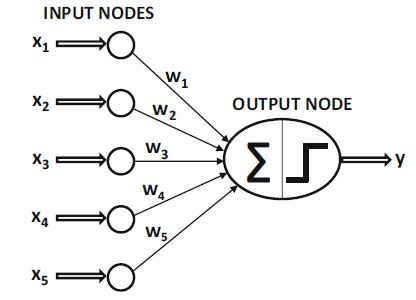
\includegraphics[width=\textwidth]{Bilder/perceptron_ohne_bias}
		%\caption{Perzeptron ohne Bias}
		%\label{fig:perceptron_ohne_bias}	
	\end{minipage}

	%\newpage
	
	
	
		Das Ziel eines Perzeptrons ist es , mit den extern angelegten Werte $x_{1},x_{2},x_{3}, \ldots ,x_{n}$ in eine von zwei Klassen, $c1$ oder $c2$, richtig zu klassifizieren. Die Entscheidungsregel für die Klassifizierung erfolgt bei eingegebenen Werten $x_{1},x_{2},x_{3}, \ldots ,x_{n}$ dann, wenn der Ausgangswert $y=1$ ist, Klasse C1 einordnen, wenn aber $y=-1$ ist , dann Klasse C2 einordnen. Die Entscheidungsregionen werden durch Hyperebene eng. \textit{hyperplane} getrennt, die mit $\sum_{i=1}^{n}w_{i}x_{i} + b = 0$ \autoref{fig:classc1_c2} definiert ist. \cite{haykin1994neural}
		
		\begin{wrapfigure}{l}{0.5\textwidth}
			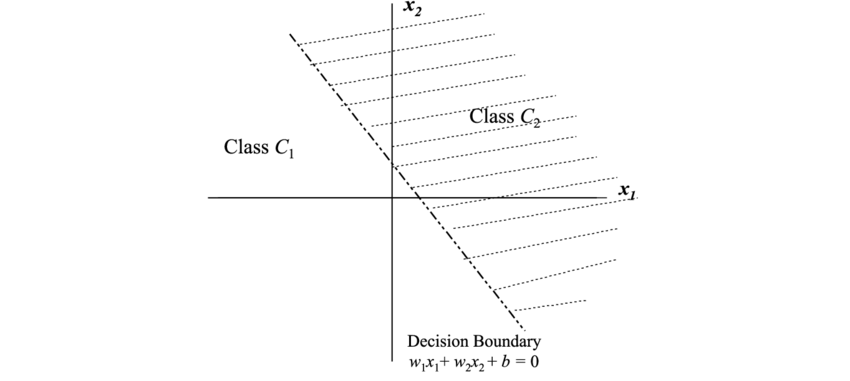
\includegraphics[width=1\linewidth]{Bilder/classc1_c2} 
			\caption{Entscheidungsregionen}
			\label{fig:classc1_c2}
		\end{wrapfigure}
		
		
		Einschichtige Netze sind die einfachsten Strukturen der künstlichen neuronaler Netze, die auch als Rosenblatts Perzeptron bezeichnet wird. Die Arbeit von Frank Rosenblatt \cite{RosenblattsPerceptron} wurde im Jahr 1958 veröffentlicht und sein Ziel war den Prognosefehler des Perzeptrons zu minimieren. Der Algorithmus wurde heuristisch entworfen, um die Anzahl von der falschen Klassifizierung zu minimieren.\\
	
	\begin{minipage}{.5\linewidth}
		\centering
		\begin{tabular}{|c|c|c|c|}
			\hline
			$x_{1}$ & $x_{2}$ & $y_{3}$ (carry) & $y_{4}$ (sum) \\ \hline
			0 & 0 & 0 & 1 \\ \hline
			0 & 1 & 0 & 1 \\ \hline
			1 & 0 & 0 & 1 \\ \hline
			1 & 1 & 1 & 0 \\ \hline
		\end{tabular}
	\end{minipage}
	\begin{minipage}[h!]{.5\linewidth}
		\centering
		% Graphic for TeX using PGF
% Title: C:\Users\Ahmet\Desktop\BachelorArbeit\ausarbeitung_tex_kit_2016\Ausarbeitung_TeX_KIT\designs\perceptron_2ein_2aus.dia
% Creator: Dia v0.97.2
% CreationDate: Sat Jan 25 20:25:04 2020
% For: Ahmet
% \usepackage{tikz}
% The following commands are not supported in PSTricks at present
% We define them conditionally, so when they are implemented,
% this pgf file will use them.
\ifx\du\undefined
  \newlength{\du}
\fi
\setlength{\du}{15\unitlength}
\begin{tikzpicture}
\pgftransformxscale{1.000000}
\pgftransformyscale{-1.000000}
\definecolor{dialinecolor}{rgb}{0.000000, 0.000000, 0.000000}
\pgfsetstrokecolor{dialinecolor}
\definecolor{dialinecolor}{rgb}{1.000000, 1.000000, 1.000000}
\pgfsetfillcolor{dialinecolor}
\pgfsetlinewidth{0.050000\du}
\pgfsetdash{}{0pt}
\pgfsetdash{}{0pt}
\pgfsetbuttcap
\pgfsetmiterjoin
\pgfsetlinewidth{0.050000\du}
\pgfsetbuttcap
\pgfsetmiterjoin
\pgfsetdash{}{0pt}
\definecolor{dialinecolor}{rgb}{1.000000, 1.000000, 1.000000}
\pgfsetfillcolor{dialinecolor}
\fill (5.032258\du,6.100000\du)--(5.032258\du,8.100000\du)--(6.967742\du,8.100000\du)--(6.967742\du,6.100000\du)--cycle;
\definecolor{dialinecolor}{rgb}{0.000000, 0.000000, 0.000000}
\pgfsetstrokecolor{dialinecolor}
\draw (5.032258\du,6.100000\du)--(5.032258\du,8.100000\du)--(6.967742\du,8.100000\du)--(6.967742\du,6.100000\du)--cycle;
\pgfsetbuttcap
\pgfsetmiterjoin
\pgfsetdash{}{0pt}
\definecolor{dialinecolor}{rgb}{0.000000, 0.000000, 0.000000}
\pgfsetstrokecolor{dialinecolor}
\draw (5.032258\du,6.100000\du)--(5.032258\du,8.100000\du)--(6.967742\du,8.100000\du)--(6.967742\du,6.100000\du)--cycle;
\pgfsetlinewidth{0.050000\du}
\pgfsetdash{}{0pt}
\pgfsetdash{}{0pt}
\pgfsetbuttcap
\pgfsetmiterjoin
\pgfsetlinewidth{0.050000\du}
\pgfsetbuttcap
\pgfsetmiterjoin
\pgfsetdash{}{0pt}
\definecolor{dialinecolor}{rgb}{1.000000, 1.000000, 1.000000}
\pgfsetfillcolor{dialinecolor}
\fill (4.975000\du,10.020000\du)--(4.975000\du,12.020000\du)--(6.910484\du,12.020000\du)--(6.910484\du,10.020000\du)--cycle;
\definecolor{dialinecolor}{rgb}{0.000000, 0.000000, 0.000000}
\pgfsetstrokecolor{dialinecolor}
\draw (4.975000\du,10.020000\du)--(4.975000\du,12.020000\du)--(6.910484\du,12.020000\du)--(6.910484\du,10.020000\du)--cycle;
\pgfsetbuttcap
\pgfsetmiterjoin
\pgfsetdash{}{0pt}
\definecolor{dialinecolor}{rgb}{0.000000, 0.000000, 0.000000}
\pgfsetstrokecolor{dialinecolor}
\draw (4.975000\du,10.020000\du)--(4.975000\du,12.020000\du)--(6.910484\du,12.020000\du)--(6.910484\du,10.020000\du)--cycle;
% setfont left to latex
\definecolor{dialinecolor}{rgb}{0.000000, 0.000000, 0.000000}
\pgfsetstrokecolor{dialinecolor}
\node at (6.000000\du,7.100000\du){1};
% setfont left to latex
\definecolor{dialinecolor}{rgb}{0.000000, 0.000000, 0.000000}
\pgfsetstrokecolor{dialinecolor}
\node at (5.942742\du,11.020000\du){2};
\definecolor{dialinecolor}{rgb}{1.000000, 1.000000, 1.000000}
\pgfsetfillcolor{dialinecolor}
\pgfpathellipse{\pgfpoint{12.613508\du}{7.028298\du}}{\pgfpoint{1.456779\du}{0\du}}{\pgfpoint{0\du}{0.981096\du}}
\pgfusepath{fill}
\pgfsetlinewidth{0.050000\du}
\pgfsetdash{}{0pt}
\pgfsetdash{}{0pt}
\definecolor{dialinecolor}{rgb}{0.000000, 0.000000, 0.000000}
\pgfsetstrokecolor{dialinecolor}
\pgfpathellipse{\pgfpoint{12.613508\du}{7.028298\du}}{\pgfpoint{1.456779\du}{0\du}}{\pgfpoint{0\du}{0.981096\du}}
\pgfusepath{stroke}
\definecolor{dialinecolor}{rgb}{1.000000, 1.000000, 1.000000}
\pgfsetfillcolor{dialinecolor}
\pgfpathellipse{\pgfpoint{12.697968\du}{11.031196\du}}{\pgfpoint{1.456779\du}{0\du}}{\pgfpoint{0\du}{0.981096\du}}
\pgfusepath{fill}
\pgfsetlinewidth{0.050000\du}
\pgfsetdash{}{0pt}
\pgfsetdash{}{0pt}
\definecolor{dialinecolor}{rgb}{0.000000, 0.000000, 0.000000}
\pgfsetstrokecolor{dialinecolor}
\pgfpathellipse{\pgfpoint{12.697968\du}{11.031196\du}}{\pgfpoint{1.456779\du}{0\du}}{\pgfpoint{0\du}{0.981096\du}}
\pgfusepath{stroke}
\pgfsetlinewidth{0.050000\du}
\pgfsetdash{}{0pt}
\pgfsetdash{}{0pt}
\pgfsetbuttcap
{
\definecolor{dialinecolor}{rgb}{0.000000, 0.000000, 0.000000}
\pgfsetfillcolor{dialinecolor}
% was here!!!
\pgfsetarrowsend{latex}
\definecolor{dialinecolor}{rgb}{0.000000, 0.000000, 0.000000}
\pgfsetstrokecolor{dialinecolor}
\draw (6.992695\du,7.086197\du)--(11.156729\du,7.028298\du);
}
\pgfsetlinewidth{0.050000\du}
\pgfsetdash{}{0pt}
\pgfsetdash{}{0pt}
\pgfsetbuttcap
{
\definecolor{dialinecolor}{rgb}{0.000000, 0.000000, 0.000000}
\pgfsetfillcolor{dialinecolor}
% was here!!!
\pgfsetarrowsend{latex}
\definecolor{dialinecolor}{rgb}{0.000000, 0.000000, 0.000000}
\pgfsetstrokecolor{dialinecolor}
\draw (6.910484\du,11.020000\du)--(11.241189\du,11.031196\du);
}
\pgfsetlinewidth{0.050000\du}
\pgfsetdash{}{0pt}
\pgfsetdash{}{0pt}
\pgfsetbuttcap
{
\definecolor{dialinecolor}{rgb}{0.000000, 0.000000, 0.000000}
\pgfsetfillcolor{dialinecolor}
% was here!!!
\pgfsetarrowsend{latex}
\definecolor{dialinecolor}{rgb}{0.000000, 0.000000, 0.000000}
\pgfsetstrokecolor{dialinecolor}
\draw (6.967742\du,7.100000\du)--(11.667870\du,10.337456\du);
}
\pgfsetlinewidth{0.050000\du}
\pgfsetdash{}{0pt}
\pgfsetdash{}{0pt}
\pgfsetbuttcap
{
\definecolor{dialinecolor}{rgb}{0.000000, 0.000000, 0.000000}
\pgfsetfillcolor{dialinecolor}
% was here!!!
\pgfsetarrowsend{latex}
\definecolor{dialinecolor}{rgb}{0.000000, 0.000000, 0.000000}
\pgfsetstrokecolor{dialinecolor}
\draw (6.910484\du,11.020000\du)--(11.583409\du,7.722037\du);
}
% setfont left to latex
\definecolor{dialinecolor}{rgb}{0.000000, 0.000000, 0.000000}
\pgfsetstrokecolor{dialinecolor}
\node at (12.613508\du,7.028298\du){3};
% setfont left to latex
\definecolor{dialinecolor}{rgb}{0.000000, 0.000000, 0.000000}
\pgfsetstrokecolor{dialinecolor}
\node at (12.697968\du,11.031196\du){4};
\end{tikzpicture}

%		\caption[Perceptron mit 2 Eingänge und 2 Ausgänge ]{Ein Perceptron Netzwerk mit 2 Eingänge und 2 Ausgänge}
	\end{minipage}\\

	Wir wollen jetz ein Perzeptron ''beibringen'', dass das 2-Bit addieren lernt. Oben links steht die Wertetabelle für ein Halbaddierer. Es gibt zwei Eingänge und 2 Ausgänge. Ein Ausgang steht für \textbf{\textit{carry}} und der zweite Ausgang für Summe \textbf{\textit{sum}}. Auf der rechten Seite sieht man die Einheiten. Die Einheit \textbf{3} ist für \textbf{\textit{carry}} und die \textbf{4.} Einheit ist für die Summe \textbf{\textit{sum}}. Die \textbf{Einheit 3} lernt die carry-Funktion leicht, weil es hier lediglich um \textbf{AND}-Operator geht. Aber die \textbf{Einheit 4} scheint nicht zu funktionieren. Die Einheit soll \textbf{XOR} \textit{(exklusive ODER)} lernen. Das Perzeptron kann aber \textbf{XOR} \textit{(exklusive ODER)} nicht lernen, weil die nicht linear trennbar ist. \autoref{fig:Entscheidungsgrenzen} \cite{russell2016artificial}
	
	\begin{figure}[h!]
		\centering
		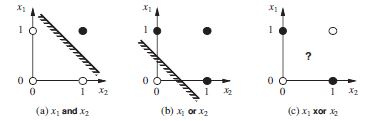
\includegraphics[width=12cm , height= 3.5 cm]{Bilder/entscheidungsgrenzen}
		\caption{Entscheidungsgrenzen von logischen Gattern}
		\label{fig:Entscheidungsgrenzen}	
	\end{figure}

	\subsection{Mehrschichtiges feedforward-Netz}\label{Mehrschichtiges feedforward-Netz}
	Das einlagige Perzeptron oder auch Rosenblatts Perzeptron enthält keine versteckten Neuronen somit kann nicht  linear trennbare Eingabemuster klassifizieren. siehe \autoref{fig:Entscheidungsgrenzen} \textit{\textbf{XOR-Problem}} Das XOR-Problem oder allgemeine Beschränkung des einlagigen Perzeptrons konnte mit dem mehrlagigen Perzeptron gelöst werden, bei dem es neben der Ausgabeschicht auch noch weitere Schicht verdeckter Neuronen engl. \textit{hidden layers} gibt.  Beim feedforward-Netz verläuft der Informationsfluss nur in einer Richtung. Ein Rekurrentes neuronales Netz ist auch möglich, falls die Neuronen im Netz, die mit Neuronen der vorangegangenen Schicht verbunden sind.  Es gibt:
	
	\begin{description}
		\item[Fully connected]\label{item:fully connected} Die Neuronen einer Schicht werden mit allen Neuronen der nächsten folgenden Schicht verbunden. \autoref{fig:MLP}
		
		\item[Short-Cuts] Einige Neuronen einer Schicht werden nicht mit allen Neuronen der nächsten folgenden Schicht verbunden, sondern mit Neuronen im übernächsten Schichten. 
		
	\end{description}
	\begin{figure}[h!]
		\centering
		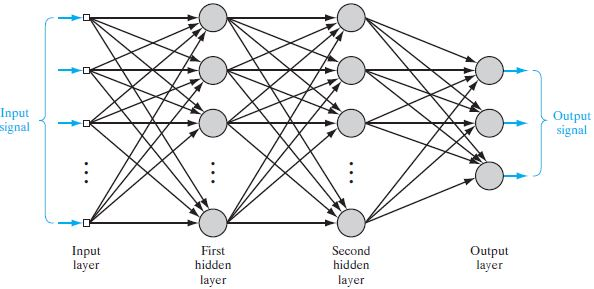
\includegraphics[width=10 cm , height=5cm]{Bilder/MLP}
		\caption{Struktur eines mehrschichtigen feedforward-Netzes}
		\label{fig:MLP}		
	\end{figure}
\newpage
	\subsection{Convolutional Neural Network}
	
	Convolutional Neural Network (\textbf{CNN} oder \textbf{ConvNet}) ist eine beliebteste Technik der künstlichen neuronalen Netzwerke (KNN) für hochdimensionale Daten wie z.B. Bilder und Videos. Ein wesenticher Unterschied zwischen CNN und allgemeine neuronalen Netzen besteht darin, dass jede Einheit in einer CNN-Schicht ein 2-dimensionales oder hoch-dimensionales Filter gibt, das mit der Eingabe dieser Schicht gefaltet wird. D.h. ein CNN kann als Eingang in Form einer Matrix verarbeiten, aber MLP siehe \autoref{Mehrschichtiges feedforward-Netz} ist nicht in der Lage eine eingegebene Matrix zu verarbeiten, da MLP einen Vektor als Input benötigt, um die Matrix zu verarbeiten. Außerdem die Pixelwerte des Bildes müssen hintereinander ausgerollt werden (Flattening). Dadurch sind normale neuronale Netze sind nicht in der Lage, Objekte in einem Bild unabhängig von der Position zu erkennen. \cite{AGuidetoConvolutional} 
	%Es gibt auch Studienarbeiten, die zeigen, dass CNN nicht nur bei der Bildverarbeitung eingesetz, sondern auch bei der Textverarbeitung. 
	
	
	\begin{description}
		\item[Ein-und Ausgänge] Wenn ein Computer ein Bild sieht, dann sieht er nicht wie Menschen \autoref{fig:hunde}, sondern einer Reihe von Pixelwerten und zwar eine Matrix. \autoref{fig:hunde_matrix} Jede dieser Zahlen von Matrix erhält einen Wert zwischen 0 und 255. Die einzelne Zahlen beschreiben die Intensität des Pixels. Diese Zahlen haben keine Bedeutung bei der Bildklassifizierung. Wofür werden dann Pixelwerte gebraucht? Die Idee ist, dass der Computer aus den Pixelwerten die Wahrscheinlichkeit berechnet und entscheidet mithilfe von Wahrscheinlichkeitswert, was in dem Bild zu sehen ist. (z.B. 0.80 Hund, 0.15 Katzen 0.05 Vogel) In diesem Beispiel die Wahrscheinichkeit bei Hunden ist größer als die anderen und entscheidet das CNN für ''Hunden''.
	\end{description}

%\begin{minipage}[t]{0.3\textwidth}
%	\centering
%	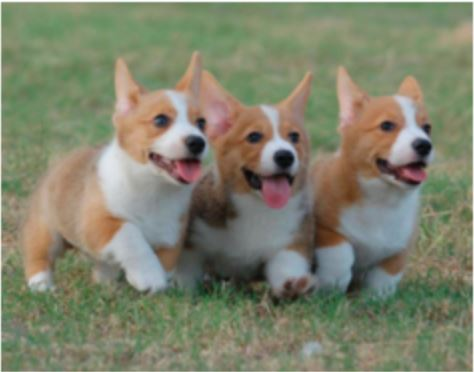
\includegraphics[width=\textwidth]{Bilder/hunde}
%	\caption{Was wir sehen}
%	\label{fig:hunde}
%\end{minipage}
%\begin{minipage}[t]{0.3\textwidth}
%	\centering
%	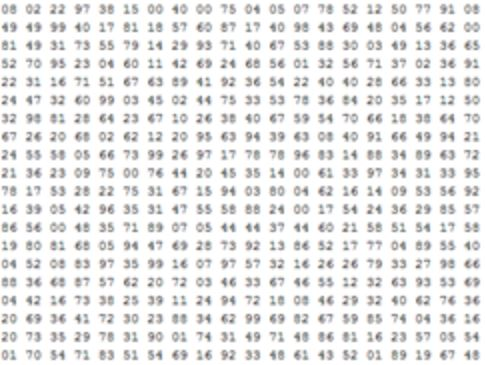
\includegraphics[width=\textwidth]{Bilder/hunde_matrix}
%	\caption{Was der Computer sieht}
%	\label{fig:hunde_matrix}
%	
%\end{minipage}

\begin{figure}
	\begin{minipage}[b]{.4\linewidth} % [b] => Ausrichtung an \caption
		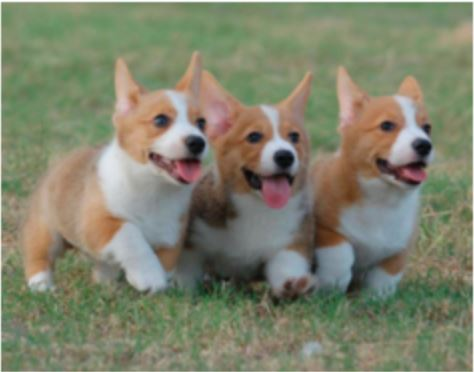
\includegraphics[width=\textwidth]{Bilder/hunde}
		\caption{Was wir sehen}
		\label{fig:hunde}
	\end{minipage}
	\hspace{.1\linewidth}% Abstand zwischen Bilder
	\begin{minipage}[b]{.4\linewidth} % [b] => Ausrichtung an \caption
		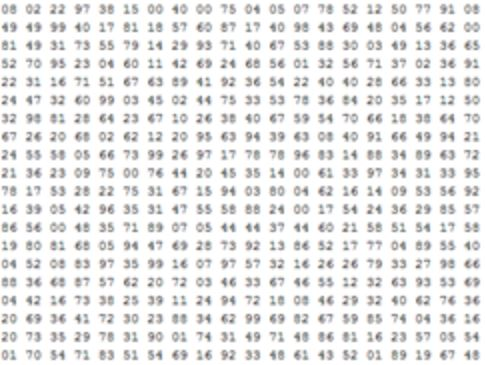
\includegraphics[width=\textwidth]{Bilder/hunde_matrix}
		\caption{Was der Computer sieht}
		\label{fig:hunde_matrix}
	\end{minipage}
\end{figure}


%\begin{figure}[h!]
%	\centering
%	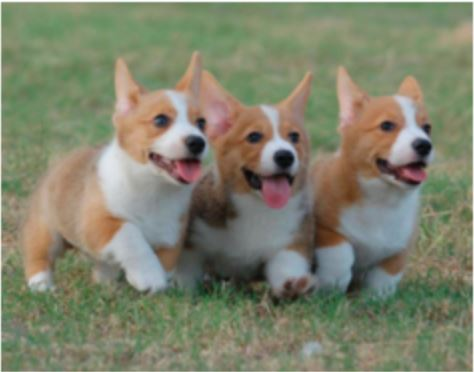
\includegraphics[width=3 cm , height=3cm]{Bilder/hunde}
%	\caption{Was wir sehen}
%	\label{fig:hunde}
%\end{figure}
%\begin{figure}
%	\centering
%	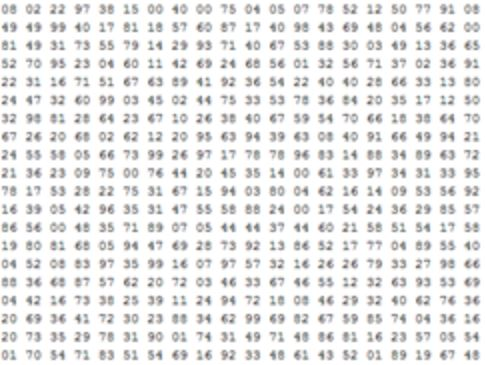
\includegraphics[width=3 cm , height=3cm]{Bilder/hunde_matrix}
%	\caption{Was der Computer sieht}
%	\label{fig:hunde_matrix}
%\end{figure}
\newpage



	\subsubsection{Struktur von Convolutional Neural Network}\label{subsubsec:Struktur von Convolutional Neural Network}
	Ein CNN besteht aus mehreren Schichten \textit{(Convoutional Layer)} \autoref{fig:cnn}, die grundlegende Funktionen wie Normalisierung, Pooling und Faltung besitzen. Die schichten wiederholen sich abwechselnd und am Ende der CNN-Schichten befindet sich ein fully connected Neuronen siehe \autoref{item:fully connected} 	
	\begin{figure}[h!]
		\centering
		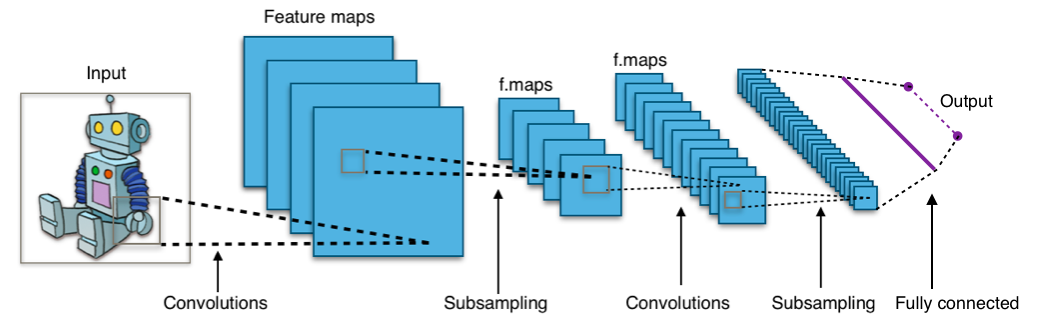
\includegraphics[width=10 cm , height=5cm]{Bilder/cnn}
		\caption{Struktur von Convolutional Neural Network CNN}
		\label{fig:cnn}		
	\end{figure}

	\subsubsection{Filter in Convolutional Layer}\label{subsubsec:Convolutional Layer}
	Eine Convolution Layer ist die wichtigste Komponente eines CNN. Die Eingabe einer Matrix (Array von Pixelwerte eines Bildes) wird zunächst von Filter in Convolutional Layers analysiert, die eine feste Pixelgröße \textit{(Kernel-size)} besitzen. Über die Pixelwerte des Bildes bzw. Matrix wandern die Filter mit einem konstanten Schrittweite von Links nach Rechts. Am Rand der Zeile von Pixelwerte springen die Filter in die nächste tiefere Zeile. Mit dem sogenannten \textit{Padding} wird festgelegt, wie sich die Filter am Rand der Matrix verhalten soll. Im \autoref{subsec:2D-Faltung} wird die Berechnungsmethode von Faltung erläutert. \\
	
	In der ersten Ebene eines CNN befinden sich 16 oder 32  Filter und nach der Faltung entsteht eine neue Matrix als Output. Danach folgt ein Pooling layer, die auch in TPU \autoref{subsec:Architektur der Tensor Processing Unit} \autoref{fig:pooling_layer} verwendet wird.
	
	\subsubsection{Pooling Layer}\label{subsubsec:Pooling Layer}
	Es gibt zwei Arten von Pooling. Die sind Max-und Average \textit{(Mittelwert)} Pooling. In CNN wird Max-Pooling angewendet. Der höchste Wert von der Kernel-Matrix weitergegeben und Rest ignoriert. Somit werden die relevantesten Signale für die nächsten Schichten ausgewählt und die Anzahl der Parameter eines Netzes reduziert. \autoref{fig:max_pooling}
	\\
	
	\begin{figure}[h!]
		\centering
		\definecolor{c1}{HTML}{9ACFC6}
\definecolor{c2}{HTML}{DABBD6}
\definecolor{c3}{HTML}{CBDCB9}
\definecolor{c4}{HTML}{9AC3E1}
\definecolor{c5}{HTML}{DEBBA5}
\definecolor{c6}{HTML}{C4DDE5}
\newcommand*{\xMin}{0}%
\newcommand*{\xMax}{6}%
\newcommand*{\yMin}{0}%
\newcommand*{\yMax}{4}%

\newcommand*{\xMinR}{9.5}%
\newcommand*{\xMaxR}{12.5}%
\newcommand*{\yMinR}{1}%
\newcommand*{\yMaxR}{3}%

\begin{tikzpicture}
    \fill [c1] (0, 0) rectangle (2, 2);
    \fill [c2]   (2, 0) rectangle (4, 2);
    \fill [c3]  (4, 0) rectangle (6, 2);
    \fill [c4] (0, 2) rectangle (2, 4);
    \fill [c5]   (2, 2) rectangle (4, 4);
    \fill [c6]   (4, 2) rectangle (6, 4);

    \fill [c1]  (9.5, 1) rectangle (10.5, 2);
    \fill [c2]   (10.5, 1) rectangle (11.5, 2);
    \fill [c3]  (11.5, 1) rectangle (12.5, 2);
    \fill [c4]  (9.5, 2) rectangle (10.5, 3);
    \fill [c5]   (10.5, 2) rectangle (11.5, 3);
    \fill [c6]   (11.5, 2) rectangle (12.5, 3);

    \foreach \i in {\xMin,...,\xMax} {
        \draw [very thin,gray] (\i,\yMin) -- (\i,\yMax)  node [below] at (\i,\yMin) {};
    }
    \foreach \i in {\yMin,...,\yMax} {
        \draw [very thin,gray] (\xMin,\i) -- (\xMax,\i) node [left] at (\xMin,\i) {};
    }

    \foreach \i in {\xMin,2,...,\xMax} {
        \draw [thick,gray] (\i,\yMin) -- (\i,\yMax)  node [below] at (\i,\yMin) {};
    }
    \foreach \i in {\yMin,2,...,\yMax} {
        \draw [thick,gray] (\xMin,\i) -- (\xMax,\i) node [left] at (\xMin,\i) {};
    }
    \node at (0.5, 0.5) {7};
    \node at (1.5, 0.5) {9};
    \node at (2.5, 0.5) {3};
    \node at (3.5, 0.5) {5};
    \node at (4.5, 0.5) {9};
    \node at (5.5, 0.5) {4};
    %
    \node at (0.5, 1.5) {0};
    \node at (1.5, 1.5) {7};
    \node at (2.5, 1.5) {0};
    \node at (3.5, 1.5) {0};
    \node at (4.5, 1.5) {9};
    \node at (5.5, 1.5) {0};
    %
    \node at (0.5, 2.5) {5};
    \node at (1.5, 2.5) {0};
    \node at (2.5, 2.5) {9};
    \node at (3.5, 2.5) {3};
    \node at (4.5, 2.5) {7};
    \node at (5.5, 2.5) {5};
    %
    \node at (0.5, 3.5) {9};
    \node at (1.5, 3.5) {2};
    \node at (2.5, 3.5) {9};
    \node at (3.5, 3.5) {6};
    \node at (4.5, 3.5) {4};
    \node at (5.5, 3.5) {3};

    \draw[draw=black,line width=12pt,-{Latex[length=9mm]}] (6.5, 2)  -- (9,2);
    \node[font=\footnotesize\bfseries] at (7.7, 2.5) {$\mathbf{2\times 2}$ max pooling};

    \foreach \i in {\xMinR,...,\xMaxR} {
        \draw [thick,gray] (\i,\yMinR) -- (\i,\yMaxR)  node [below] at (\i,\yMinR) {};
    }
    \foreach \i in {\yMinR,...,\yMaxR} {
        \draw [thick,gray] (\xMinR,\i) -- (\xMaxR,\i) node [left] at (\xMinR,\i) {};
    }

    \node at (10, 1.5) {9};
    \node at (11, 1.5) {5};
    \node at (12, 1.5) {9};
    \node at (10, 2.5) {9};
    \node at (11, 2.5) {9};
    \node at (12, 2.5) {7};

    \draw [decorate,decoration={brace,amplitude=4pt},xshift=-2pt,yshift=0pt]
(0,2) -- (0,4) node [black,midway,xshift=-0.3cm] {\footnotesize $2$};

    \draw [decorate,decoration={brace,amplitude=4pt},xshift=0pt,yshift=2pt]
(0,4) -- (2,4) node [black,midway,yshift=+0.3cm] {\footnotesize $2$};
\end{tikzpicture}
		\caption[Max Pooling]{Hier ist die Kernel-Matrix 2x2, wird Maximum Wert aus dem Bereich ausgewählt und zur nächste 2x2-Matrix verschoben.  }
		\label{fig:max_pooling}		
	\end{figure}

	\subsubsection{Fully connected Layer / Dense Layer}\label{subsubsec:Fully connected Layer}
	Es handelt sich hier um eine normale neuronale Netzstruktur. Die Neuronen sind fully-connnected siehe \autoref{item:fully connected}. Alle Inputs und Outputs sind mit Neuronen verbunden. Um die Matrix aus dem Pooling Layer ins Netz speisen zu können, müssen sie zunächst ausgerollt werden (flatten). Fully Connected Layer kann die Matrix nicht verarbeiten, sondern nur die Werte der Matrix.
%	\begin{figure}[h!]
%		\centering
%		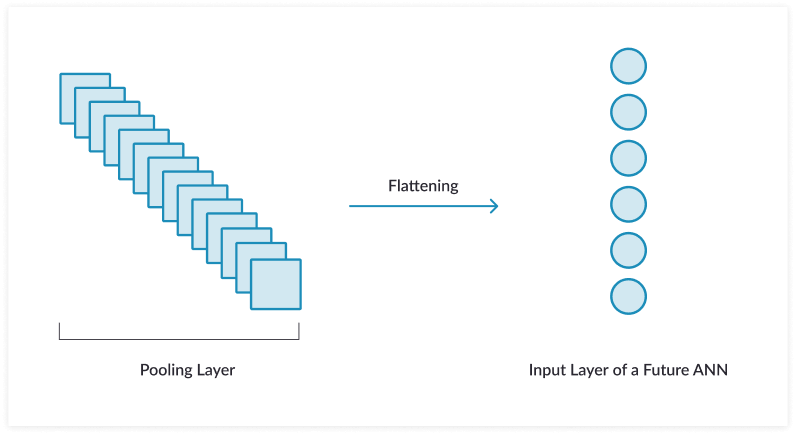
\includegraphics[width=8 cm , height=4.5cm]{Bilder/flatten}
%		\caption[Flatten]{Zwischen convolutional layer und fully-connected layer befindet sich eine ''flatten'-layer. Eine zweidimensionale Eingangsmatrix wird durch Abflachung in einen Vektor umgewandelt, damit sie ins neuronalen Netz eingespeist werden können. }
%		\label{fig:flatten}		
%	\end{figure}

\begin{wrapfigure}{l}{0.5\textwidth}
	%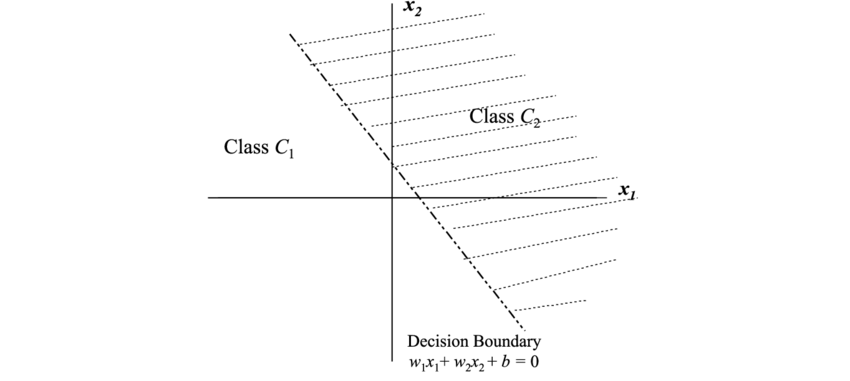
\includegraphics[width=1\linewidth]{Bilder/classc1_c2} 
	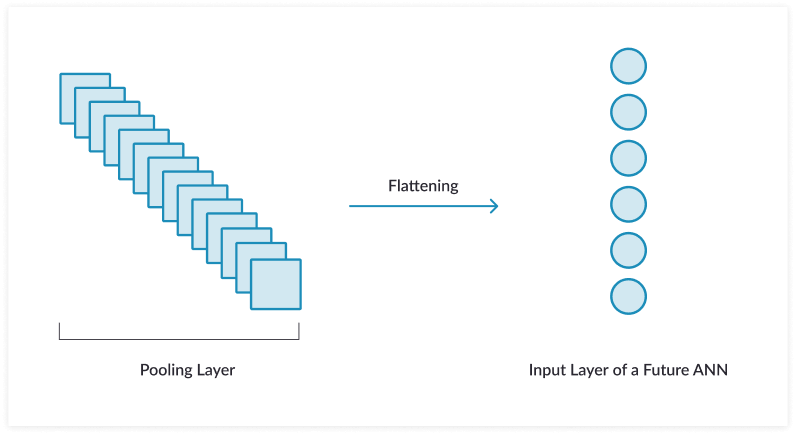
\includegraphics[width=1\linewidth]{Bilder/flatten}
\end{wrapfigure}
Zwischen convolutional layer und fully-connected layer befindet sich eine \\''flatten''-layer. Eine zweidimensionale Eingangsmatrix wird durch Abflachung in einen Vektor umgewandelt, damit sie ins neuronalen Netz eingespeist werden können.
\clearpage

\newpage

	\subsubsection{Zusammenfassung CNN}\label{subsubsec:Zusammenfassung CNN}

	Ein CNN akzeptiert als Eingang eine Matrix, die reine Intensitätswerten eines Bildes bestehen. Die Verarbeitung verläuft durch mehreren Schichten, um Strukturen, wie Linien, Kanten, Kurven etc. eines eingegebenes Bildes zu erkennen. Die Filter in Schichten von CNN sind nicht vorgegeben, sondern vom Netz gelernt. In jeder höheren Filterebene erhöht sich die Abstraktions-Level des Netzes. Es ist sehr interessant, die Muster zu visualisieren, welche jeweils auf verschiedenen Ebenen zur Aktivierung der Filter führen. \autoref{fig:layer}
	
	\begin{figure}[h!]
		\centering
		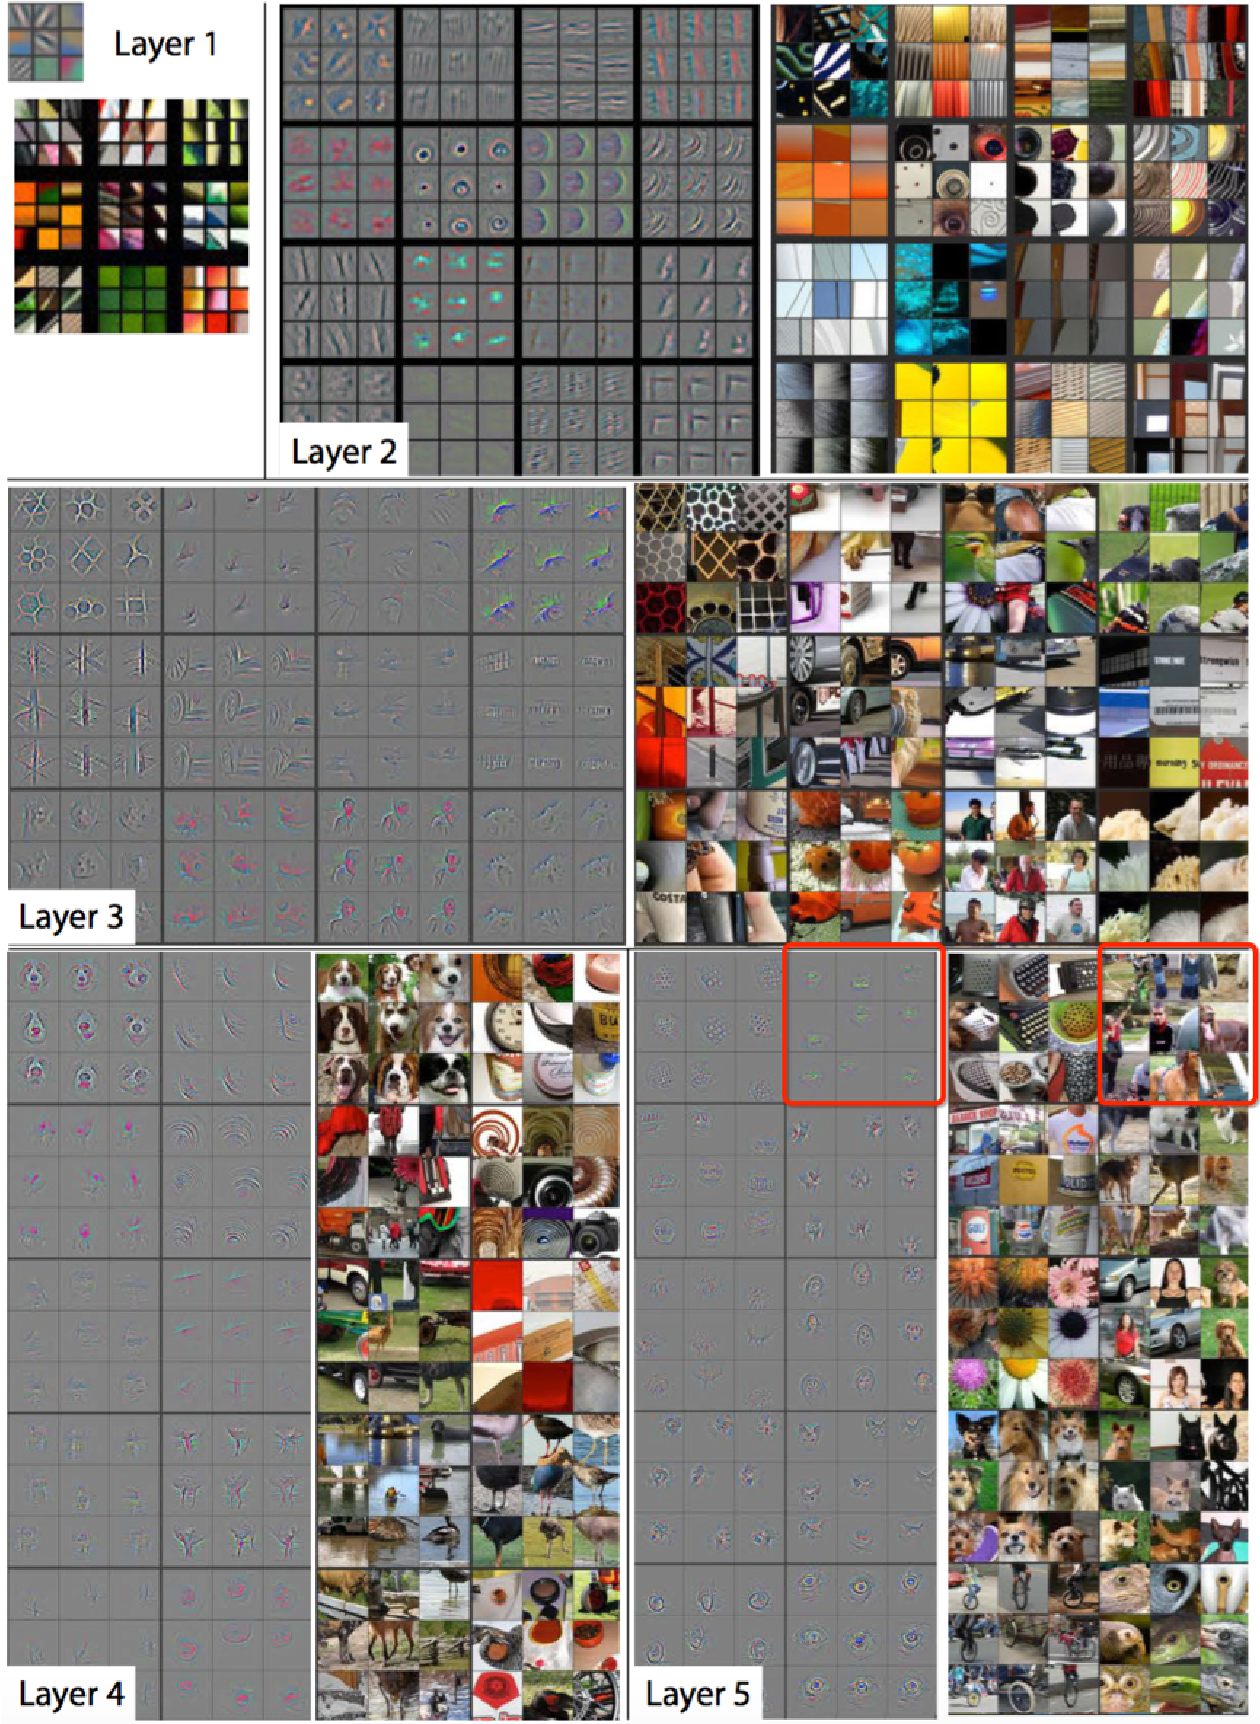
\includegraphics[width=15 cm , height=17cm]{Bilder/layer}
		\caption{Visualisierung von Convolutional Network}
		\label{fig:layer} 	
	\end{figure}

	\subsection{Beispiele von CNN Architekturen}\label{subsec:Beispiele von CNN Architekturen}
	Hier werden einige erfolgreiche CNN-Entwürfe vorgestellt, die unter Grundlagen von CNN erstellt wurden. Die einige Grundlagen sind wie Faltungen, Max-Pooling, Funktion von Fully connected layer, flatening etc. schon oben erläutert. Zuerst möchte ich mit früheren Entwurf vorstellen und anschließend folgen dann die neue davon, sodass man den Trend bei der Entwicklung von CNN-Architekturen einen Überblick bekommt.
	
	\begin{description}
		\item[LENET] Die LeNet-Architektur \cite{lecun1998gradient} ist eine der frühesten und grundlegendsten Formen von CNNs, die für die handschriftliche Ziffernidentifikation entwickelt wurde. \cite{AGuidetoConvolutional} Die erfolgreichste Variante dieser Architektur ist die LeNet-5 Modell, da es insgesamt 5 Gewichtsschichten umfasst. LeNet besteht aus zwei convolutional layer, denen jeweils eine (Max-Pooling)-Schicht folgt, um Merkmale zu extrahieren. Anschließend folgt eine einzelne convolution layer. Am Ende des Modells befinden sich dann fully-connected layer.
		Die Modellarchitektur ist in \autoref{fig:lenet}  dargestellt.
		
		\begin{figure}[h!]
			\centering
			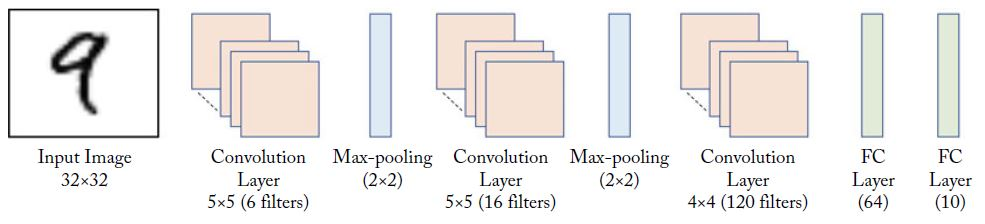
\includegraphics[width=15 cm , height=5cm]{Bilder/lenet5}
			\caption{LeNet-5 Architektur \cite{lecun1998gradient}}
			\label{fig:lenet} 
		\end{figure}
	
	%%fertig


		\item[AlexNet] Im Jahr 2012 gewann AlexNet \cite{ImageNet} Architektur mit einem besonderen Erfolg im Vergleich zu den anderen Architekturen die ImageNet Large-Scale Visual Recognition Challenge (ILSVRC). \footnote{http://www.image-net.org/} 
		AlexNet besteht aus insgesamt acht Parameterschichten, von denen die fünf convolution layer und drei Fully connected Layer sind. Die letzte Fully-connected Layer klassifiziert das Eingangsbild in einer der 1000 Klassen von ImageNet-Dataset. Die Filtergrößen und die Position der Max-Pooling layer sind in \autoref{fig:alexnet} dargestellt.
		Die Verwendung der nichtlineare Funktionen nach jeder convolutional layer verbessert die Trainingseffizienz im Vergleich zur traditionell verwendeten $\tanh$-Funktionen.
	
		
		\begin{figure}[h!]
			\centering
			\includegraphics[width=15 cm , height=5cm]{Bilder/alexnet}
			\caption{AlexNet Architektur \cite{AGuidetoConvolutional}}
			\label{fig:alexnet} 
		\end{figure}
	
	\newpage
	
	\item[GoogleNet] Bisher diskutierten Netzwerke bestehen aus einer sequentiellen Architektur in  einer Richtung. Entlang dieser Richtung befinden sich nach Reihen geordnet Schichten wie convolution layer , Max-pooling, ReLu und Fully-connected layer etc. Die GoogleNet-Architektur \cite{szegedy2015going} ist eine komplexe Architektur mit mehreren Netzwerkzweigen und gewann den ILSVRC (Large Scale Visual Recognition Challenge) im Jahr 2014 mit der Fehlerquote von 6,7\% bei der Klassifizierungsaufgabe. 
	GoogleNet \autoref{fig:GoogleNet} besteht aus insgesamt 22 Gewichtsschichten und das Grundkonzept ist das ''Inception-Module''.
	Die Verarbeitung dieses Moduls erfolgt im Vergleich bisher vorgestellten Architekturen nicht sequentiell, sondern parallel. Eine einfache Version dieses Moduls ist in \autoref{fig:GoogleNet} dargestellt. \\ Die Hauptidee von GoogleNet ist, alle grundlegenden Verarbeitungsblöcke, die in einem regulären sequentiellen CNN auftreten, parallel zu platzieren und die Ausgaben davon kombinieren. Der Vorteil von GoogleNet ist, dass mehrere ''Inception-Module''  zusammen gestapelt werden, um ein riesigen Netzwerk zu erstellen. 
	
	\begin{figure}[h!]
		\centering
		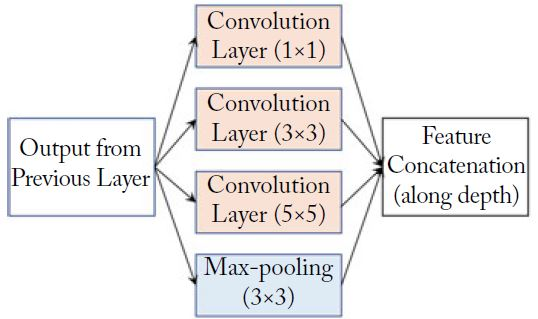
\includegraphics[width=10 cm , height=4cm]{Bilder/googleNet}
		\caption{Grundkonzept von GoogleNet Inception Module \cite{szegedy2015going}}
		\label{fig:GoogleNet} 
	\end{figure}
	
	Ein großes Problem beim ''Inception Module'' ist, dass die Faltungen wie 5x5 auf einer convolutional layer mit einer großen Anzahl von Filtern sehr ineffizient sein kann. Das wird noch deutlicher, wenn dazu Pooling-Einheiten hinzugefügt werden. Die Anzahl der Ausgangsfilter entspricht der Anzahl der Filter in der vorherigen Stufen. Beim Mischen der Ausgabe der pooling-Unit mit den Ausgaben der convolutional layer würde die Anzahl von Ausgaben von Stufe zu Stufe extrem zunehmen. Innerhalb wenige Stufen könnte dies zu einer rechnerischen Explosion führen und die Ausgaben können höhere Dimensionen haben. Um dieses Problem zu überwinden, müssen die Dimension der Ausgaben reduziert werden. \autoref{fig:dimensionred}
	siehe mehr Details zur Lösung \cite{szegedy2015going}
	
	\begin{figure}[h!]
		\centering
		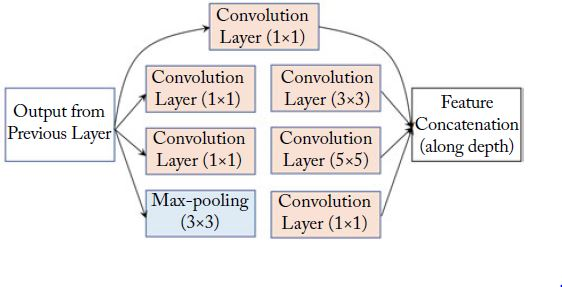
\includegraphics[width=10 cm , height=4cm]{Bilder/dimensionred}
		\caption[GoogleNet Inception Module]{Neues Inception-Modul, um Dimensionen von Ausgaben  zu reduzieren \cite{szegedy2015going}}
		\label{fig:dimensionred} 
	\end{figure}

	
	
\end{description}
	
	

	\chapter{Konzept}\label{ch:Konzept}  	
	\section{Einfuehrung der Systolic Array Architektur}\label{sec:Einfuehrung der Systolic Array Architektur}
	Machine Learning basiert stark auf Berechnungen z.B. von Faltungen, Matrix-Matrix-und Matrix-Vektor Multiplikationen, Berechnung von Verlustfunktionen, Max-Pooling usw. siehe \autoref{ch:Grundlagen} \\Die künstliche neuronale Netze bestehen aus vielen kuenstlichen Neuronen, indem viele Berechnungen stattfinden, die den Ausgabewert des ML-Modells beeinflussen. 
	Das wesentliche Ziel ist die Entwicklung neuer Rechnerarchitektur und der effizienten Nutzung von modernen Systeme, um solchen komplizierten ML-Anwendungen schneller ausführen zu können. Die wachsende Nachfrage nach mehr Rechenleistung führte in den 80er Jahren zur Entwicklung parallel skalierbaren Multiprocessing-Systemen. Das System soll durch paralleles Rechnen in der Lage sein, dass ein kompliziertes großes Rechenproblem in kleinere Stück unterteilt und diese kleine Rechenprobleme gleichzeitig löst. \cite{DesignofSystolicArchitecture}
	
	\textbf{Problem der sequentille Berechnungsmethode: }Bei der herkömmlichen Berechnungsmethode der Matrix-Matrix Multiplikationen \autoref{fig:mm} wird zuerst überprüft, ob die Matrizen miteinander multiplizierbar sind. D.h. wenn die Spaltenanzahl von A-Matrix mit der Zeilenanzahl von B-Matrix übereinstimmen, dann sind sie miteinander multiplizierbar. Der Nachteil dieser Berechnungsmethode ist die sequentielle Ausführung von Rechenoperationen, die sehr zeitaufwändig ist. Es findet keine zeitgleiche bzw. parallele Berechnung statt. Das Ziel ist aber ein Algorithmus zu entwickeln, dass parallele Berechnung und sogar mehrere parallele Berechnungen durchführt, sodass die Rechenleistung erhöht wird.


	\begin{figure}[h!]
		\centering
			\definecolor{myyellow}{RGB}{240,217,1}
		\definecolor{mygreen}{RGB}{143,188,103}
		\definecolor{myred}{RGB}{234,38,40}
		\definecolor{myblue}{RGB}{53,101,167}
		
			\begin{tikzpicture}[
		mymatrix/.style={
			matrix of math nodes,
			outer sep=0pt,
			nodes={
				draw,
				text width=2.5em,
				align=center,
				minimum height=2.5em,
				text=gray
			},
			nodes in empty cells,
			column sep=-\pgflinewidth,
			row sep=-\pgflinewidth,
			left delimiter=[,
			right delimiter=],
		},
		mycircle/.style 2 args={
			draw=#1,
			circle,
			fill=#2,
			line width=2pt,
			inner sep=5pt
		},
		arr/.style={
			line width=4pt,
			-{Triangle[angle=60:1.5pt 3]},
			#1,
			shorten >= 3pt,
			shorten <= 3pt
		}
		]
		%the matrices
		\matrix[mymatrix] (A)
		{
			|[text=black]|a_{11} & |[text=black]|a_{12} \\
			a_{21} & a_{22} \\
			|[text=black]|a_{31} & |[text=black]|a_{32} \\
			a_{41} & a_{42} \\
		};
		\matrix[mymatrix,right=of A.north east,anchor=north west] (prod)
		{
			& & \\
			& & \\
			& & \\
			& & \\
		};
		\matrix[mymatrix,above=of prod.north west,anchor=south west] (B)
		{
			b_{11} & |[text=black]|b_{12} & |[text=black]|b_{13} \\
			b_{21} & |[text=black]|b_{22} & |[text=black]|b_{23} \\
		};
		
		%the labels for the matrices
		\node[font=\huge,left=10pt of A] {$A$};
		\node[font=\huge,above=2pt of B] {$B$};
		
		%the frames in both matrices
		\draw[myyellow,line width=2pt]
		([shift={(1.2pt,-1.2pt)}]A-1-1.north west) 
		rectangle 
		([shift={(-1.2pt,1.2pt)}]A-1-2.south east);
		\draw[myyellow,line width=2pt]
		([shift={(1.2pt,-1.2pt)}]B-1-2.north west) 
		rectangle 
		([shift={(-1.2pt,1.2pt)}]B-2-2.south east);
		\draw[mygreen,line width=2pt]
		([shift={(1.2pt,-1.2pt)}]A-3-1.north west) 
		rectangle 
		([shift={(-1.2pt,1.2pt)}]A-3-2.south east);
		\draw[mygreen,line width=2pt]
		([shift={(1.2pt,-1.2pt)}]B-1-3.north west) 
		rectangle 
		([shift={(-1.2pt,1.2pt)}]B-2-3.south east);
		
		%the filled circles in the product
		\node[mycircle={myblue}{mygreen}]
		at (prod-3-3) (prod33) {};
		\node[mycircle={myred}{myyellow}]
		at (prod-1-2) (prod12) {};
		
		%the arrows
		\draw[arr=myred]
		(A-1-2.east) -- (prod12); 
		\draw[arr=myred]
		(B-2-2.south) -- (prod12); 
		\draw[arr=myblue]
		(A-3-2.east) -- (prod33); 
		\draw[arr=myblue]
		(B-2-3.south) -- (prod33); 
		
		%the legend
		\matrix[
		matrix of math nodes,
		nodes in empty cells,
		column sep=10pt,
		anchor=north,
		nodes={
			minimum height=2.2em,
			minimum width=2em,
			anchor=north west
		},
		below=5pt of current bounding box.south
		] 
		(legend)
		{
			& a_{11}b_{12} + a_{12}b_{22} \\
			& a_{31}b_{13} + a_{32}b_{23} \\
		};
		\node[mycircle={myblue}{mygreen}]
		at (legend-2-1) {};
		\node[mycircle={myred}{myyellow}]
		at (legend-1-1) {};
		\end{tikzpicture}
		\caption{Matrix Multiplikation}
		\label{fig:mm}		
	\end{figure}


	
	

	
	\section{Why Systolic Architectures?} \label{sec:Why Systolic Architectures?}
	\subsection{Grundidee}\label{subsec:Grundidee}
%	Der Begriff ''systolisches Array'' kann nach einer neuen Innovation in der Rechnerarchitektur klingen.Aber es ist fast 40 Jahre alt. H.T. Kung kam auf diese Idee in den 80er Jahren und veröffentlichte seine Idee im Jahr 1982.\footnote{http://www.eecs.harvard.edu/~htk/publication/1982-kung-why-systolic-architecture.pdf}
	
	Die Grundidee des systolischen Arrays \cite{kung1982systolic} ist, dass die Daten rhythmisch aus dem Computerspeicher fließen und laufen durch viele PEs (processing elements), bevor sie in den Speicher zurückkehren. Die Idee ist vergleichbar mit dem Blutkreislauf, dass der Herz zur Zellen Blut pumpt.
	%\newpage
	
	
%	\begin{center}
%		%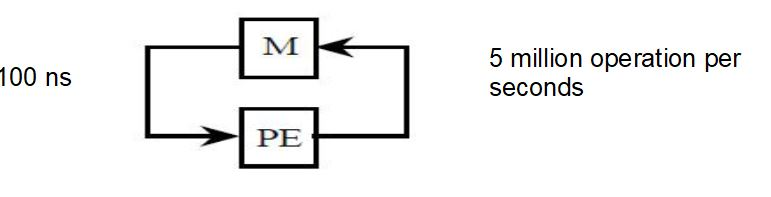
\includegraphics[width=12 cm , height= 5 cm]{Bilder/einPE}
%		% Graphic for TeX using PGF
% Title: C:\WINDOWS\system32\Diagramm2.dia
% Creator: Dia v0.97.2
% CreationDate: Sun Jan 12 13:08:28 2020
% For: Ahmet
% \usepackage{tikz}
% The following commands are not supported in PSTricks at present
% We define them conditionally, so when they are implemented,
% this pgf file will use them.
\ifx\du\undefined
  \newlength{\du}
\fi
\setlength{\du}{15\unitlength}
\begin{tikzpicture}
\pgftransformxscale{1.000000}
\pgftransformyscale{-1.000000}
\definecolor{dialinecolor}{rgb}{0.000000, 0.000000, 0.000000}
\pgfsetstrokecolor{dialinecolor}
\definecolor{dialinecolor}{rgb}{1.000000, 1.000000, 1.000000}
\pgfsetfillcolor{dialinecolor}
\pgfsetlinewidth{0.050000\du}
\pgfsetdash{}{0pt}
\pgfsetdash{}{0pt}
\pgfsetmiterjoin
\definecolor{dialinecolor}{rgb}{1.000000, 1.000000, 1.000000}
\pgfsetfillcolor{dialinecolor}
\fill (9.800000\du,8.000000\du)--(9.800000\du,10.100000\du)--(11.900000\du,10.100000\du)--(11.900000\du,8.000000\du)--cycle;
\definecolor{dialinecolor}{rgb}{0.000000, 0.000000, 0.000000}
\pgfsetstrokecolor{dialinecolor}
\draw (9.800000\du,8.000000\du)--(9.800000\du,10.100000\du)--(11.900000\du,10.100000\du)--(11.900000\du,8.000000\du)--cycle;
\pgfsetlinewidth{0.050000\du}
\pgfsetdash{}{0pt}
\pgfsetdash{}{0pt}
\pgfsetmiterjoin
\definecolor{dialinecolor}{rgb}{1.000000, 1.000000, 1.000000}
\pgfsetfillcolor{dialinecolor}
\fill (8.900000\du,5.350000\du)--(8.900000\du,6.650000\du)--(12.750000\du,6.650000\du)--(12.750000\du,5.350000\du)--cycle;
\definecolor{dialinecolor}{rgb}{0.000000, 0.000000, 0.000000}
\pgfsetstrokecolor{dialinecolor}
\draw (8.900000\du,5.350000\du)--(8.900000\du,6.650000\du)--(12.750000\du,6.650000\du)--(12.750000\du,5.350000\du)--cycle;
% setfont left to latex
\definecolor{dialinecolor}{rgb}{0.000000, 0.000000, 0.000000}
\pgfsetstrokecolor{dialinecolor}
\node at (10.825000\du,6.075000\du){Speicher};
% setfont left to latex
\definecolor{dialinecolor}{rgb}{0.000000, 0.000000, 0.000000}
\pgfsetstrokecolor{dialinecolor}
\node at (10.850000\du,9.272500\du){PE};
\pgfsetlinewidth{0.050000\du}
\pgfsetdash{}{0pt}
\pgfsetdash{}{0pt}
\pgfsetmiterjoin
\pgfsetbuttcap
{
\definecolor{dialinecolor}{rgb}{0.000000, 0.000000, 0.000000}
\pgfsetfillcolor{dialinecolor}
% was here!!!
\pgfsetarrowsend{stealth}
{\pgfsetcornersarced{\pgfpoint{0.000000\du}{0.000000\du}}\definecolor{dialinecolor}{rgb}{0.000000, 0.000000, 0.000000}
\pgfsetstrokecolor{dialinecolor}
\draw (8.900000\du,6.000000\du)--(7.875000\du,6.000000\du)--(7.875000\du,9.050000\du)--(9.774738\du,9.050000\du);
}}
\pgfsetlinewidth{0.050000\du}
\pgfsetdash{}{0pt}
\pgfsetdash{}{0pt}
\pgfsetmiterjoin
\pgfsetbuttcap
{
\definecolor{dialinecolor}{rgb}{0.000000, 0.000000, 0.000000}
\pgfsetfillcolor{dialinecolor}
% was here!!!
\pgfsetarrowsend{stealth}
{\pgfsetcornersarced{\pgfpoint{0.000000\du}{0.000000\du}}\definecolor{dialinecolor}{rgb}{0.000000, 0.000000, 0.000000}
\pgfsetstrokecolor{dialinecolor}
\draw (11.900000\du,9.050000\du)--(14.100000\du,9.050000\du)--(14.100000\du,6.000000\du)--(12.750000\du,6.000000\du);
}}
% setfont left to latex
\definecolor{dialinecolor}{rgb}{0.000000, 0.000000, 0.000000}
\pgfsetstrokecolor{dialinecolor}
\node[anchor=west] at (5.500000\du,7.600000\du){100 ns};
% setfont left to latex
\definecolor{dialinecolor}{rgb}{0.000000, 0.000000, 0.000000}
\pgfsetstrokecolor{dialinecolor}
\node[anchor=west] at (14.750000\du,7.400000\du){5 million operation };
% setfont left to latex
\definecolor{dialinecolor}{rgb}{0.000000, 0.000000, 0.000000}
\pgfsetstrokecolor{dialinecolor}
\node[anchor=west] at (14.750000\du,8.200000\du){per second (MOPS)};
\end{tikzpicture}

%	\end{center}

	\begin{figure}
		\begin{center}
			% Graphic for TeX using PGF
% Title: C:\WINDOWS\system32\Diagramm2.dia
% Creator: Dia v0.97.2
% CreationDate: Sun Jan 12 13:08:28 2020
% For: Ahmet
% \usepackage{tikz}
% The following commands are not supported in PSTricks at present
% We define them conditionally, so when they are implemented,
% this pgf file will use them.
\ifx\du\undefined
  \newlength{\du}
\fi
\setlength{\du}{15\unitlength}
\begin{tikzpicture}
\pgftransformxscale{1.000000}
\pgftransformyscale{-1.000000}
\definecolor{dialinecolor}{rgb}{0.000000, 0.000000, 0.000000}
\pgfsetstrokecolor{dialinecolor}
\definecolor{dialinecolor}{rgb}{1.000000, 1.000000, 1.000000}
\pgfsetfillcolor{dialinecolor}
\pgfsetlinewidth{0.050000\du}
\pgfsetdash{}{0pt}
\pgfsetdash{}{0pt}
\pgfsetmiterjoin
\definecolor{dialinecolor}{rgb}{1.000000, 1.000000, 1.000000}
\pgfsetfillcolor{dialinecolor}
\fill (9.800000\du,8.000000\du)--(9.800000\du,10.100000\du)--(11.900000\du,10.100000\du)--(11.900000\du,8.000000\du)--cycle;
\definecolor{dialinecolor}{rgb}{0.000000, 0.000000, 0.000000}
\pgfsetstrokecolor{dialinecolor}
\draw (9.800000\du,8.000000\du)--(9.800000\du,10.100000\du)--(11.900000\du,10.100000\du)--(11.900000\du,8.000000\du)--cycle;
\pgfsetlinewidth{0.050000\du}
\pgfsetdash{}{0pt}
\pgfsetdash{}{0pt}
\pgfsetmiterjoin
\definecolor{dialinecolor}{rgb}{1.000000, 1.000000, 1.000000}
\pgfsetfillcolor{dialinecolor}
\fill (8.900000\du,5.350000\du)--(8.900000\du,6.650000\du)--(12.750000\du,6.650000\du)--(12.750000\du,5.350000\du)--cycle;
\definecolor{dialinecolor}{rgb}{0.000000, 0.000000, 0.000000}
\pgfsetstrokecolor{dialinecolor}
\draw (8.900000\du,5.350000\du)--(8.900000\du,6.650000\du)--(12.750000\du,6.650000\du)--(12.750000\du,5.350000\du)--cycle;
% setfont left to latex
\definecolor{dialinecolor}{rgb}{0.000000, 0.000000, 0.000000}
\pgfsetstrokecolor{dialinecolor}
\node at (10.825000\du,6.075000\du){Speicher};
% setfont left to latex
\definecolor{dialinecolor}{rgb}{0.000000, 0.000000, 0.000000}
\pgfsetstrokecolor{dialinecolor}
\node at (10.850000\du,9.272500\du){PE};
\pgfsetlinewidth{0.050000\du}
\pgfsetdash{}{0pt}
\pgfsetdash{}{0pt}
\pgfsetmiterjoin
\pgfsetbuttcap
{
\definecolor{dialinecolor}{rgb}{0.000000, 0.000000, 0.000000}
\pgfsetfillcolor{dialinecolor}
% was here!!!
\pgfsetarrowsend{stealth}
{\pgfsetcornersarced{\pgfpoint{0.000000\du}{0.000000\du}}\definecolor{dialinecolor}{rgb}{0.000000, 0.000000, 0.000000}
\pgfsetstrokecolor{dialinecolor}
\draw (8.900000\du,6.000000\du)--(7.875000\du,6.000000\du)--(7.875000\du,9.050000\du)--(9.774738\du,9.050000\du);
}}
\pgfsetlinewidth{0.050000\du}
\pgfsetdash{}{0pt}
\pgfsetdash{}{0pt}
\pgfsetmiterjoin
\pgfsetbuttcap
{
\definecolor{dialinecolor}{rgb}{0.000000, 0.000000, 0.000000}
\pgfsetfillcolor{dialinecolor}
% was here!!!
\pgfsetarrowsend{stealth}
{\pgfsetcornersarced{\pgfpoint{0.000000\du}{0.000000\du}}\definecolor{dialinecolor}{rgb}{0.000000, 0.000000, 0.000000}
\pgfsetstrokecolor{dialinecolor}
\draw (11.900000\du,9.050000\du)--(14.100000\du,9.050000\du)--(14.100000\du,6.000000\du)--(12.750000\du,6.000000\du);
}}
% setfont left to latex
\definecolor{dialinecolor}{rgb}{0.000000, 0.000000, 0.000000}
\pgfsetstrokecolor{dialinecolor}
\node[anchor=west] at (5.500000\du,7.600000\du){100 ns};
% setfont left to latex
\definecolor{dialinecolor}{rgb}{0.000000, 0.000000, 0.000000}
\pgfsetstrokecolor{dialinecolor}
\node[anchor=west] at (14.750000\du,7.400000\du){5 million operation };
% setfont left to latex
\definecolor{dialinecolor}{rgb}{0.000000, 0.000000, 0.000000}
\pgfsetstrokecolor{dialinecolor}
\node[anchor=west] at (14.750000\du,8.200000\du){per second (MOPS)};
\end{tikzpicture}

		\end{center}
		\caption[Einzelne Processing Elemente PEs]{\label{fig:SA_1PE} Das Grundprinzip des systolischen Systems}
	\end{figure}

	Das in \autoref{fig:SA_1PE} Verarbeitungsschema ist ineffizient und zeitaufwändig, wenn es nur ein einziges PE gibt, das aus dem Speicher ein Data holt, verarbeitet und das Ergebnis in den Speicher ablegt. In einer Sekunde werden nur 5 Millionen Operationen \textbf{MOPS} \textit{(Millions of operations per seconds)} durchgeführt.  

  
	Um \textbf{MOPS} zu erhöhen soll mehrere PEs geben, die Daten mehrmals verarbeiten (wie Pipeline System) und am Ende das Ergebnis wird von dem letzten PE in den Speicher abgelegt. \autoref{fig:PEs} Das ist die Idee, die das System beschleunigen soll. Damit werden 30 Millionen Operationen durchgeführt.


	\begin{figure}
		\begin{center}
			% Graphic for TeX using PGF
% Title: C:\WINDOWS\system32\Diagramm3.dia
% Creator: Dia v0.97.2
% CreationDate: Sun Jan 12 13:15:05 2020
% For: Ahmet
% \usepackage{tikz}
% The following commands are not supported in PSTricks at present
% We define them conditionally, so when they are implemented,
% this pgf file will use them.
\ifx\du\undefined
  \newlength{\du}
\fi
\setlength{\du}{15\unitlength}
\begin{tikzpicture}
\pgftransformxscale{1.000000}
\pgftransformyscale{-1.000000}
\definecolor{dialinecolor}{rgb}{0.000000, 0.000000, 0.000000}
\pgfsetstrokecolor{dialinecolor}
\definecolor{dialinecolor}{rgb}{1.000000, 1.000000, 1.000000}
\pgfsetfillcolor{dialinecolor}
\pgfsetlinewidth{0.050000\du}
\pgfsetdash{}{0pt}
\pgfsetdash{}{0pt}
\pgfsetmiterjoin
\definecolor{dialinecolor}{rgb}{1.000000, 1.000000, 1.000000}
\pgfsetfillcolor{dialinecolor}
\fill (5.080846\du,6.804735\du)--(5.080846\du,8.904735\du)--(7.180846\du,8.904735\du)--(7.180846\du,6.804735\du)--cycle;
\definecolor{dialinecolor}{rgb}{0.000000, 0.000000, 0.000000}
\pgfsetstrokecolor{dialinecolor}
\draw (5.080846\du,6.804735\du)--(5.080846\du,8.904735\du)--(7.180846\du,8.904735\du)--(7.180846\du,6.804735\du)--cycle;
\pgfsetlinewidth{0.050000\du}
\pgfsetdash{}{0pt}
\pgfsetdash{}{0pt}
\pgfsetmiterjoin
\definecolor{dialinecolor}{rgb}{1.000000, 1.000000, 1.000000}
\pgfsetfillcolor{dialinecolor}
\fill (8.924584\du,2.965475\du)--(8.924584\du,4.265475\du)--(12.774584\du,4.265475\du)--(12.774584\du,2.965475\du)--cycle;
\definecolor{dialinecolor}{rgb}{0.000000, 0.000000, 0.000000}
\pgfsetstrokecolor{dialinecolor}
\draw (8.924584\du,2.965475\du)--(8.924584\du,4.265475\du)--(12.774584\du,4.265475\du)--(12.774584\du,2.965475\du)--cycle;
% setfont left to latex
\definecolor{dialinecolor}{rgb}{0.000000, 0.000000, 0.000000}
\pgfsetstrokecolor{dialinecolor}
\node at (10.849584\du,3.465475\du){Speicher};
% setfont left to latex
\definecolor{dialinecolor}{rgb}{0.000000, 0.000000, 0.000000}
\pgfsetstrokecolor{dialinecolor}
\node at (6.130846\du,8.077235\du){PE};
% setfont left to latex
\definecolor{dialinecolor}{rgb}{0.000000, 0.000000, 0.000000}
\pgfsetstrokecolor{dialinecolor}
\node[anchor=west] at (1.507264\du,5.636471\du){100 ns};
\pgfsetlinewidth{0.050000\du}
\pgfsetdash{}{0pt}
\pgfsetdash{}{0pt}
\pgfsetmiterjoin
\definecolor{dialinecolor}{rgb}{1.000000, 1.000000, 1.000000}
\pgfsetfillcolor{dialinecolor}
\fill (8.019512\du,6.796571\du)--(8.019512\du,8.896571\du)--(10.119512\du,8.896571\du)--(10.119512\du,6.796571\du)--cycle;
\definecolor{dialinecolor}{rgb}{0.000000, 0.000000, 0.000000}
\pgfsetstrokecolor{dialinecolor}
\draw (8.019512\du,6.796571\du)--(8.019512\du,8.896571\du)--(10.119512\du,8.896571\du)--(10.119512\du,6.796571\du)--cycle;
% setfont left to latex
\definecolor{dialinecolor}{rgb}{0.000000, 0.000000, 0.000000}
\pgfsetstrokecolor{dialinecolor}
\node at (9.069512\du,8.069071\du){PE};
\pgfsetlinewidth{0.050000\du}
\pgfsetdash{}{0pt}
\pgfsetdash{}{0pt}
\pgfsetmiterjoin
\definecolor{dialinecolor}{rgb}{1.000000, 1.000000, 1.000000}
\pgfsetfillcolor{dialinecolor}
\fill (11.002244\du,6.772314\du)--(11.002244\du,8.872314\du)--(13.102244\du,8.872314\du)--(13.102244\du,6.772314\du)--cycle;
\definecolor{dialinecolor}{rgb}{0.000000, 0.000000, 0.000000}
\pgfsetstrokecolor{dialinecolor}
\draw (11.002244\du,6.772314\du)--(11.002244\du,8.872314\du)--(13.102244\du,8.872314\du)--(13.102244\du,6.772314\du)--cycle;
% setfont left to latex
\definecolor{dialinecolor}{rgb}{0.000000, 0.000000, 0.000000}
\pgfsetstrokecolor{dialinecolor}
\node at (12.052244\du,8.044814\du){PE};
\pgfsetlinewidth{0.050000\du}
\pgfsetdash{}{0pt}
\pgfsetdash{}{0pt}
\pgfsetmiterjoin
\definecolor{dialinecolor}{rgb}{1.000000, 1.000000, 1.000000}
\pgfsetfillcolor{dialinecolor}
\fill (17.085746\du,6.764150\du)--(17.085746\du,8.864150\du)--(19.185746\du,8.864150\du)--(19.185746\du,6.764150\du)--cycle;
\definecolor{dialinecolor}{rgb}{0.000000, 0.000000, 0.000000}
\pgfsetstrokecolor{dialinecolor}
\draw (17.085746\du,6.764150\du)--(17.085746\du,8.864150\du)--(19.185746\du,8.864150\du)--(19.185746\du,6.764150\du)--cycle;
% setfont left to latex
\definecolor{dialinecolor}{rgb}{0.000000, 0.000000, 0.000000}
\pgfsetstrokecolor{dialinecolor}
\node at (18.135746\du,8.036650\du){PE};
\pgfsetlinewidth{0.050000\du}
\pgfsetdash{{\pgflinewidth}{0.200000\du}}{0cm}
\pgfsetdash{{\pgflinewidth}{0.200000\du}}{0cm}
\pgfsetbuttcap
{
\definecolor{dialinecolor}{rgb}{0.000000, 0.000000, 0.000000}
\pgfsetfillcolor{dialinecolor}
% was here!!!
\definecolor{dialinecolor}{rgb}{0.000000, 0.000000, 0.000000}
\pgfsetstrokecolor{dialinecolor}
\draw (13.102244\du,7.822314\du)--(14.948933\du,7.810681\du);
}
\pgfsetlinewidth{0.050000\du}
\pgfsetdash{}{0pt}
\pgfsetdash{}{0pt}
\pgfsetbuttcap
{
\definecolor{dialinecolor}{rgb}{0.000000, 0.000000, 0.000000}
\pgfsetfillcolor{dialinecolor}
% was here!!!
\pgfsetarrowsend{latex}
\definecolor{dialinecolor}{rgb}{0.000000, 0.000000, 0.000000}
\pgfsetstrokecolor{dialinecolor}
\draw (14.948933\du,7.794470\du)--(17.072500\du,7.794470\du);
}
\pgfsetlinewidth{0.050000\du}
\pgfsetdash{}{0pt}
\pgfsetdash{}{0pt}
\pgfsetbuttcap
{
\definecolor{dialinecolor}{rgb}{0.000000, 0.000000, 0.000000}
\pgfsetfillcolor{dialinecolor}
% was here!!!
\pgfsetarrowsend{latex}
\definecolor{dialinecolor}{rgb}{0.000000, 0.000000, 0.000000}
\pgfsetstrokecolor{dialinecolor}
\draw (7.180846\du,7.854735\du)--(8.019512\du,7.846571\du);
}
\pgfsetlinewidth{0.050000\du}
\pgfsetdash{}{0pt}
\pgfsetdash{}{0pt}
\pgfsetbuttcap
{
\definecolor{dialinecolor}{rgb}{0.000000, 0.000000, 0.000000}
\pgfsetfillcolor{dialinecolor}
% was here!!!
\pgfsetarrowsend{latex}
\definecolor{dialinecolor}{rgb}{0.000000, 0.000000, 0.000000}
\pgfsetstrokecolor{dialinecolor}
\draw (10.119512\du,7.846571\du)--(11.002244\du,7.822314\du);
}
\pgfsetlinewidth{0.050000\du}
\pgfsetdash{}{0pt}
\pgfsetdash{}{0pt}
\pgfsetmiterjoin
\pgfsetbuttcap
{
\definecolor{dialinecolor}{rgb}{0.000000, 0.000000, 0.000000}
\pgfsetfillcolor{dialinecolor}
% was here!!!
\pgfsetarrowsend{latex}
{\pgfsetcornersarced{\pgfpoint{0.000000\du}{0.000000\du}}\definecolor{dialinecolor}{rgb}{0.000000, 0.000000, 0.000000}
\pgfsetstrokecolor{dialinecolor}
\draw (8.924584\du,3.615475\du)--(4.055846\du,3.615475\du)--(4.055846\du,7.854735\du)--(5.080846\du,7.854735\du);
}}
\pgfsetlinewidth{0.050000\du}
\pgfsetdash{}{0pt}
\pgfsetdash{}{0pt}
\pgfsetmiterjoin
\pgfsetbuttcap
{
\definecolor{dialinecolor}{rgb}{0.000000, 0.000000, 0.000000}
\pgfsetfillcolor{dialinecolor}
% was here!!!
\pgfsetarrowsend{latex}
{\pgfsetcornersarced{\pgfpoint{0.000000\du}{0.000000\du}}\definecolor{dialinecolor}{rgb}{0.000000, 0.000000, 0.000000}
\pgfsetstrokecolor{dialinecolor}
\draw (19.185746\du,7.814150\du)--(20.210746\du,7.814150\du)--(20.210746\du,3.615475\du)--(12.774584\du,3.615475\du);
}}
% setfont left to latex
\definecolor{dialinecolor}{rgb}{0.000000, 0.000000, 0.000000}
\pgfsetstrokecolor{dialinecolor}
\node[anchor=west] at (20.847810\du,5.468293\du){30 million operation };
% setfont left to latex
\definecolor{dialinecolor}{rgb}{0.000000, 0.000000, 0.000000}
\pgfsetstrokecolor{dialinecolor}
\node[anchor=west] at (20.847810\du,6.268293\du){per seconds};
\end{tikzpicture}

		\end{center}
		\caption[Mehrere Processing Elemente PEs]{\label{fig:PEs} Das Grundprinzip des systolischen Systems}
	\end{figure}
	
	
	\subsection{Systolic Array Designs für Faltung Berechnungen}
	
	\textbf{Design1: Gegeben} sind hier die Eingangswerte $\left[ x_{1}, x_{2},\ldots ,x_{n}\right]$  und\\ die Gewichte $\left[ w_{1}, w_{2},\ldots ,w_{k}\right]$.\\
	Die Ausgangswerte sind $y_{i} = \left[ w_{1}x_{i}+w_{2}x_{i+1}+ \ldots + w_{k}x_{i+k-1} \right]$.\\
	Die Gewichte sind schon in jeder Zelle vorgeladen. Die Eingangswerte $x_{i}$ verbreiten sich zu jeder Zelle, wird multipliziert mit der Gewichte und Teilsummen $y_{i}$ bewegen sich systolisch durch jede Zelle. \autoref{fig:design1}
	
	\begin{figure}[h!]
		\centering
		% Graphic for TeX using PGF
% Title: C:\Users\Ahmet\Desktop\BachelorArbeit\ausarbeitung_tex_kit_2016\Ausarbeitung_TeX_KIT\designs\Design1\Diagramm1.dia
% Creator: Dia v0.97.2
% CreationDate: Sat Jan 18 12:24:12 2020
% For: Ahmet
% \usepackage{tikz}
% The following commands are not supported in PSTricks at present
% We define them conditionally, so when they are implemented,
% this pgf file will use them.
\ifx\du\undefined
  \newlength{\du}
\fi
\setlength{\du}{15\unitlength}
\begin{tikzpicture}
\pgftransformxscale{1.000000}
\pgftransformyscale{-1.000000}
\definecolor{dialinecolor}{rgb}{0.000000, 0.000000, 0.000000}
\pgfsetstrokecolor{dialinecolor}
\definecolor{dialinecolor}{rgb}{1.000000, 1.000000, 1.000000}
\pgfsetfillcolor{dialinecolor}
\pgfsetlinewidth{0.050000\du}
\pgfsetdash{}{0pt}
\pgfsetdash{}{0pt}
\pgfsetbuttcap
\pgfsetmiterjoin
\pgfsetlinewidth{0.050000\du}
\pgfsetbuttcap
\pgfsetmiterjoin
\pgfsetdash{}{0pt}
\definecolor{dialinecolor}{rgb}{1.000000, 1.000000, 1.000000}
\pgfsetfillcolor{dialinecolor}
\fill (5.080889\du,7.951369\du)--(5.080889\du,9.951369\du)--(7.016373\du,9.951369\du)--(7.016373\du,7.951369\du)--cycle;
\definecolor{dialinecolor}{rgb}{0.000000, 0.000000, 0.000000}
\pgfsetstrokecolor{dialinecolor}
\draw (5.080889\du,7.951369\du)--(5.080889\du,9.951369\du)--(7.016373\du,9.951369\du)--(7.016373\du,7.951369\du)--cycle;
\pgfsetbuttcap
\pgfsetmiterjoin
\pgfsetdash{}{0pt}
\definecolor{dialinecolor}{rgb}{0.000000, 0.000000, 0.000000}
\pgfsetstrokecolor{dialinecolor}
\draw (5.080889\du,7.951369\du)--(5.080889\du,9.951369\du)--(7.016373\du,9.951369\du)--(7.016373\du,7.951369\du)--cycle;
\pgfsetlinewidth{0.050000\du}
\pgfsetdash{}{0pt}
\pgfsetdash{}{0pt}
\pgfsetbuttcap
\pgfsetmiterjoin
\pgfsetlinewidth{0.050000\du}
\pgfsetbuttcap
\pgfsetmiterjoin
\pgfsetdash{}{0pt}
\definecolor{dialinecolor}{rgb}{1.000000, 1.000000, 1.000000}
\pgfsetfillcolor{dialinecolor}
\fill (9.153177\du,7.945000\du)--(9.153177\du,9.945000\du)--(11.088661\du,9.945000\du)--(11.088661\du,7.945000\du)--cycle;
\definecolor{dialinecolor}{rgb}{0.000000, 0.000000, 0.000000}
\pgfsetstrokecolor{dialinecolor}
\draw (9.153177\du,7.945000\du)--(9.153177\du,9.945000\du)--(11.088661\du,9.945000\du)--(11.088661\du,7.945000\du)--cycle;
\pgfsetbuttcap
\pgfsetmiterjoin
\pgfsetdash{}{0pt}
\definecolor{dialinecolor}{rgb}{0.000000, 0.000000, 0.000000}
\pgfsetstrokecolor{dialinecolor}
\draw (9.153177\du,7.945000\du)--(9.153177\du,9.945000\du)--(11.088661\du,9.945000\du)--(11.088661\du,7.945000\du)--cycle;
\pgfsetlinewidth{0.050000\du}
\pgfsetdash{}{0pt}
\pgfsetdash{}{0pt}
\pgfsetbuttcap
{
\definecolor{dialinecolor}{rgb}{0.000000, 0.000000, 0.000000}
\pgfsetfillcolor{dialinecolor}
% was here!!!
\pgfsetarrowsend{stealth}
\definecolor{dialinecolor}{rgb}{0.000000, 0.000000, 0.000000}
\pgfsetstrokecolor{dialinecolor}
\draw (7.016373\du,8.951369\du)--(9.153177\du,8.945000\du);
}
\pgfsetlinewidth{0.050000\du}
\pgfsetdash{}{0pt}
\pgfsetdash{}{0pt}
\pgfsetbuttcap
\pgfsetmiterjoin
\pgfsetlinewidth{0.050000\du}
\pgfsetbuttcap
\pgfsetmiterjoin
\pgfsetdash{}{0pt}
\definecolor{dialinecolor}{rgb}{1.000000, 1.000000, 1.000000}
\pgfsetfillcolor{dialinecolor}
\fill (12.870628\du,7.954815\du)--(12.870628\du,9.954815\du)--(14.806111\du,9.954815\du)--(14.806111\du,7.954815\du)--cycle;
\definecolor{dialinecolor}{rgb}{0.000000, 0.000000, 0.000000}
\pgfsetstrokecolor{dialinecolor}
\draw (12.870628\du,7.954815\du)--(12.870628\du,9.954815\du)--(14.806111\du,9.954815\du)--(14.806111\du,7.954815\du)--cycle;
\pgfsetbuttcap
\pgfsetmiterjoin
\pgfsetdash{}{0pt}
\definecolor{dialinecolor}{rgb}{0.000000, 0.000000, 0.000000}
\pgfsetstrokecolor{dialinecolor}
\draw (12.870628\du,7.954815\du)--(12.870628\du,9.954815\du)--(14.806111\du,9.954815\du)--(14.806111\du,7.954815\du)--cycle;
\pgfsetlinewidth{0.050000\du}
\pgfsetdash{}{0pt}
\pgfsetdash{}{0pt}
\pgfsetbuttcap
{
\definecolor{dialinecolor}{rgb}{0.000000, 0.000000, 0.000000}
\pgfsetfillcolor{dialinecolor}
% was here!!!
\pgfsetarrowsend{stealth}
\definecolor{dialinecolor}{rgb}{0.000000, 0.000000, 0.000000}
\pgfsetstrokecolor{dialinecolor}
\draw (11.088661\du,8.945000\du)--(12.870628\du,8.954815\du);
}
\pgfsetlinewidth{0.050000\du}
\pgfsetdash{}{0pt}
\pgfsetdash{}{0pt}
\pgfsetmiterjoin
\pgfsetbuttcap
{
\definecolor{dialinecolor}{rgb}{0.000000, 0.000000, 0.000000}
\pgfsetfillcolor{dialinecolor}
% was here!!!
\pgfsetarrowsend{stealth}
{\pgfsetcornersarced{\pgfpoint{0.000000\du}{0.000000\du}}\definecolor{dialinecolor}{rgb}{0.000000, 0.000000, 0.000000}
\pgfsetstrokecolor{dialinecolor}
\draw (3.988276\du,6.987591\du)--(3.988276\du,6.994088\du)--(13.838370\du,6.994088\du)--(13.838370\du,7.954815\du);
}}
\pgfsetlinewidth{0.050000\du}
\pgfsetdash{}{0pt}
\pgfsetdash{}{0pt}
\pgfsetbuttcap
{
\definecolor{dialinecolor}{rgb}{0.000000, 0.000000, 0.000000}
\pgfsetfillcolor{dialinecolor}
% was here!!!
\pgfsetarrowsend{stealth}
\definecolor{dialinecolor}{rgb}{0.000000, 0.000000, 0.000000}
\pgfsetstrokecolor{dialinecolor}
\draw (10.098228\du,6.994088\du)--(10.120919\du,7.945000\du);
}
\pgfsetlinewidth{0.050000\du}
\pgfsetdash{}{0pt}
\pgfsetdash{}{0pt}
\pgfsetbuttcap
{
\definecolor{dialinecolor}{rgb}{0.000000, 0.000000, 0.000000}
\pgfsetfillcolor{dialinecolor}
% was here!!!
\pgfsetarrowsend{stealth}
\definecolor{dialinecolor}{rgb}{0.000000, 0.000000, 0.000000}
\pgfsetstrokecolor{dialinecolor}
\draw (6.054980\du,6.994088\du)--(6.048631\du,7.951369\du);
}
% setfont left to latex
\definecolor{dialinecolor}{rgb}{0.000000, 0.000000, 0.000000}
\pgfsetstrokecolor{dialinecolor}
\node at (6.048631\du,8.951369\du){w1};
% setfont left to latex
\definecolor{dialinecolor}{rgb}{0.000000, 0.000000, 0.000000}
\pgfsetstrokecolor{dialinecolor}
\node at (10.120919\du,8.945000\du){w2};
% setfont left to latex
\definecolor{dialinecolor}{rgb}{0.000000, 0.000000, 0.000000}
\pgfsetstrokecolor{dialinecolor}
\node at (13.838370\du,8.954815\du){w3};
\pgfsetlinewidth{0.050000\du}
\pgfsetdash{}{0pt}
\pgfsetdash{}{0pt}
\pgfsetbuttcap
{
\definecolor{dialinecolor}{rgb}{0.000000, 0.000000, 0.000000}
\pgfsetfillcolor{dialinecolor}
% was here!!!
\pgfsetarrowsend{stealth}
\definecolor{dialinecolor}{rgb}{0.000000, 0.000000, 0.000000}
\pgfsetstrokecolor{dialinecolor}
\draw (14.806111\du,8.954815\du)--(16.822086\du,8.938262\du);
}
% setfont left to latex
\definecolor{dialinecolor}{rgb}{0.000000, 0.000000, 0.000000}
\pgfsetstrokecolor{dialinecolor}
\node[anchor=west] at (17.034216\du,9.044326\du){yi};
% setfont left to latex
\definecolor{dialinecolor}{rgb}{0.000000, 0.000000, 0.000000}
\pgfsetstrokecolor{dialinecolor}
\node at (4.529094\du,6.592064\du){x1};
\pgfsetlinewidth{0.050000\du}
\pgfsetdash{{\pgflinewidth}{0.200000\du}}{0cm}
\pgfsetdash{{\pgflinewidth}{0.200000\du}}{0cm}
\pgfsetbuttcap
{
\definecolor{dialinecolor}{rgb}{0.000000, 0.000000, 0.000000}
\pgfsetfillcolor{dialinecolor}
% was here!!!
\pgfsetarrowsend{stealth}
\definecolor{dialinecolor}{rgb}{0.000000, 0.000000, 0.000000}
\pgfsetstrokecolor{dialinecolor}
\draw (1.548792\du,6.987591\du)--(3.528663\du,6.987591\du);
}
% setfont left to latex
\definecolor{dialinecolor}{rgb}{0.000000, 0.000000, 0.000000}
\pgfsetstrokecolor{dialinecolor}
\node at (2.018899\du,6.673268\du){x2};
\pgfsetlinewidth{0.050000\du}
\pgfsetdash{{\pgflinewidth}{0.200000\du}}{0cm}
\pgfsetdash{{\pgflinewidth}{0.200000\du}}{0cm}
\pgfsetbuttcap
{
\definecolor{dialinecolor}{rgb}{0.000000, 0.000000, 0.000000}
\pgfsetfillcolor{dialinecolor}
% was here!!!
\pgfsetarrowsend{stealth}
\definecolor{dialinecolor}{rgb}{0.000000, 0.000000, 0.000000}
\pgfsetstrokecolor{dialinecolor}
\draw (-1.268738\du,6.982370\du)--(0.711133\du,6.982370\du);
}
% setfont left to latex
\definecolor{dialinecolor}{rgb}{0.000000, 0.000000, 0.000000}
\pgfsetstrokecolor{dialinecolor}
\node at (-0.767510\du,6.637913\du){x3};
\end{tikzpicture}

		\caption[Design1]{In PE gespeicherten Gewichten werden jeweils mit der Eingabe multipliziert und das Ergebnis zur Teilsumme vom vorherigen Element addiert. Beim nächsten Takt wird ein Eingangselement ausgelesen und die Teilsummen von PE wird zum Nachbar PE gesendet. Somit werden alle Daten trotz bei minimaler Bandbreite des Speichers verarbeitet.}
		\label{fig:design1}
	\end{figure}
	
	\textbf{Design2}: Die Eingangswerte $x_{i}$ verbreiten sich in Zellen und die Ausgangswerte $y_{i}$ werden in Zellen berechnet und akkumuliert. Die Gewichte $w_{i}$ bewegen sich in einer Schleife systolisch durch jede Zelle. Am Ende der Berechnung müssen die Ergebnisse $y_{i}$ aus den Zellen geholt werden. Dafür ist eine seperate BUS-Leitung nötig, um die Ergebnisse auszugeben, was im \textbf{Design1} \autoref{fig:design1} nicht der Fall war. Das Ziel vom \textbf{Design2} \autoref{fig:design2} ist die Erhöhung der Genauigkeit von Ergebnissen, da die $y_{i}$-Werte während der Berechnung wie im \textbf{Design 1} \autoref{fig:design2} in jedem Takt sich ändern oder die Genauigkeit kann bei Gleitkommazahlen sinken und das Ergebnis kann damit gefälscht werden. 


	\begin{figure}[h!]
		\centering
		% Graphic for TeX using PGF
% Title: C:\Users\Ahmet\Desktop\BachelorArbeit\ausarbeitung_tex_kit_2016\Ausarbeitung_TeX_KIT\designs\Design2\Diagramm1.dia
% Creator: Dia v0.97.2
% CreationDate: Sat Jan 18 13:29:49 2020
% For: Ahmet
% \usepackage{tikz}
% The following commands are not supported in PSTricks at present
% We define them conditionally, so when they are implemented,
% this pgf file will use them.
\ifx\du\undefined
  \newlength{\du}
\fi
\setlength{\du}{15\unitlength}
\begin{tikzpicture}
\pgftransformxscale{1.000000}
\pgftransformyscale{-1.000000}
\definecolor{dialinecolor}{rgb}{0.000000, 0.000000, 0.000000}
\pgfsetstrokecolor{dialinecolor}
\definecolor{dialinecolor}{rgb}{1.000000, 1.000000, 1.000000}
\pgfsetfillcolor{dialinecolor}
\pgfsetlinewidth{0.050000\du}
\pgfsetdash{}{0pt}
\pgfsetdash{}{0pt}
\pgfsetbuttcap
\pgfsetmiterjoin
\pgfsetlinewidth{0.050000\du}
\pgfsetbuttcap
\pgfsetmiterjoin
\pgfsetdash{}{0pt}
\definecolor{dialinecolor}{rgb}{1.000000, 1.000000, 1.000000}
\pgfsetfillcolor{dialinecolor}
\fill (18.325280\du,6.528087\du)--(18.325280\du,8.528087\du)--(20.260763\du,8.528087\du)--(20.260763\du,6.528087\du)--cycle;
\definecolor{dialinecolor}{rgb}{0.000000, 0.000000, 0.000000}
\pgfsetstrokecolor{dialinecolor}
\draw (18.325280\du,6.528087\du)--(18.325280\du,8.528087\du)--(20.260763\du,8.528087\du)--(20.260763\du,6.528087\du)--cycle;
\pgfsetbuttcap
\pgfsetmiterjoin
\pgfsetdash{}{0pt}
\definecolor{dialinecolor}{rgb}{0.000000, 0.000000, 0.000000}
\pgfsetstrokecolor{dialinecolor}
\draw (18.325280\du,6.528087\du)--(18.325280\du,8.528087\du)--(20.260763\du,8.528087\du)--(20.260763\du,6.528087\du)--cycle;
\pgfsetlinewidth{0.050000\du}
\pgfsetdash{}{0pt}
\pgfsetdash{}{0pt}
\pgfsetbuttcap
\pgfsetmiterjoin
\pgfsetlinewidth{0.050000\du}
\pgfsetbuttcap
\pgfsetmiterjoin
\pgfsetdash{}{0pt}
\definecolor{dialinecolor}{rgb}{1.000000, 1.000000, 1.000000}
\pgfsetfillcolor{dialinecolor}
\fill (22.397570\du,6.521717\du)--(22.397570\du,8.521717\du)--(24.333053\du,8.521717\du)--(24.333053\du,6.521717\du)--cycle;
\definecolor{dialinecolor}{rgb}{0.000000, 0.000000, 0.000000}
\pgfsetstrokecolor{dialinecolor}
\draw (22.397570\du,6.521717\du)--(22.397570\du,8.521717\du)--(24.333053\du,8.521717\du)--(24.333053\du,6.521717\du)--cycle;
\pgfsetbuttcap
\pgfsetmiterjoin
\pgfsetdash{}{0pt}
\definecolor{dialinecolor}{rgb}{0.000000, 0.000000, 0.000000}
\pgfsetstrokecolor{dialinecolor}
\draw (22.397570\du,6.521717\du)--(22.397570\du,8.521717\du)--(24.333053\du,8.521717\du)--(24.333053\du,6.521717\du)--cycle;
\pgfsetlinewidth{0.050000\du}
\pgfsetdash{}{0pt}
\pgfsetdash{}{0pt}
\pgfsetbuttcap
{
\definecolor{dialinecolor}{rgb}{0.000000, 0.000000, 0.000000}
\pgfsetfillcolor{dialinecolor}
% was here!!!
\pgfsetarrowsend{stealth}
\definecolor{dialinecolor}{rgb}{0.000000, 0.000000, 0.000000}
\pgfsetstrokecolor{dialinecolor}
\draw (20.260763\du,7.528087\du)--(22.397570\du,7.521717\du);
}
\pgfsetlinewidth{0.050000\du}
\pgfsetdash{}{0pt}
\pgfsetdash{}{0pt}
\pgfsetbuttcap
\pgfsetmiterjoin
\pgfsetlinewidth{0.050000\du}
\pgfsetbuttcap
\pgfsetmiterjoin
\pgfsetdash{}{0pt}
\definecolor{dialinecolor}{rgb}{1.000000, 1.000000, 1.000000}
\pgfsetfillcolor{dialinecolor}
\fill (26.114990\du,6.531527\du)--(26.114990\du,8.531527\du)--(28.050473\du,8.531527\du)--(28.050473\du,6.531527\du)--cycle;
\definecolor{dialinecolor}{rgb}{0.000000, 0.000000, 0.000000}
\pgfsetstrokecolor{dialinecolor}
\draw (26.114990\du,6.531527\du)--(26.114990\du,8.531527\du)--(28.050473\du,8.531527\du)--(28.050473\du,6.531527\du)--cycle;
\pgfsetbuttcap
\pgfsetmiterjoin
\pgfsetdash{}{0pt}
\definecolor{dialinecolor}{rgb}{0.000000, 0.000000, 0.000000}
\pgfsetstrokecolor{dialinecolor}
\draw (26.114990\du,6.531527\du)--(26.114990\du,8.531527\du)--(28.050473\du,8.531527\du)--(28.050473\du,6.531527\du)--cycle;
\pgfsetlinewidth{0.050000\du}
\pgfsetdash{}{0pt}
\pgfsetdash{}{0pt}
\pgfsetbuttcap
{
\definecolor{dialinecolor}{rgb}{0.000000, 0.000000, 0.000000}
\pgfsetfillcolor{dialinecolor}
% was here!!!
\pgfsetarrowsend{stealth}
\definecolor{dialinecolor}{rgb}{0.000000, 0.000000, 0.000000}
\pgfsetstrokecolor{dialinecolor}
\draw (24.333053\du,7.521717\du)--(26.114990\du,7.531527\du);
}
\pgfsetlinewidth{0.050000\du}
\pgfsetdash{}{0pt}
\pgfsetdash{}{0pt}
\pgfsetmiterjoin
\pgfsetbuttcap
{
\definecolor{dialinecolor}{rgb}{0.000000, 0.000000, 0.000000}
\pgfsetfillcolor{dialinecolor}
% was here!!!
\pgfsetarrowsend{stealth}
{\pgfsetcornersarced{\pgfpoint{0.000000\du}{0.000000\du}}\definecolor{dialinecolor}{rgb}{0.000000, 0.000000, 0.000000}
\pgfsetstrokecolor{dialinecolor}
\draw (17.232670\du,5.564307\du)--(17.232670\du,5.570807\du)--(27.082731\du,5.570807\du)--(27.082731\du,6.531527\du);
}}
\pgfsetlinewidth{0.050000\du}
\pgfsetdash{}{0pt}
\pgfsetdash{}{0pt}
\pgfsetbuttcap
{
\definecolor{dialinecolor}{rgb}{0.000000, 0.000000, 0.000000}
\pgfsetfillcolor{dialinecolor}
% was here!!!
\pgfsetarrowsend{stealth}
\definecolor{dialinecolor}{rgb}{0.000000, 0.000000, 0.000000}
\pgfsetstrokecolor{dialinecolor}
\draw (23.342590\du,5.570807\du)--(23.365311\du,6.521717\du);
}
\pgfsetlinewidth{0.050000\du}
\pgfsetdash{}{0pt}
\pgfsetdash{}{0pt}
\pgfsetbuttcap
{
\definecolor{dialinecolor}{rgb}{0.000000, 0.000000, 0.000000}
\pgfsetfillcolor{dialinecolor}
% was here!!!
\pgfsetarrowsend{stealth}
\definecolor{dialinecolor}{rgb}{0.000000, 0.000000, 0.000000}
\pgfsetstrokecolor{dialinecolor}
\draw (19.299370\du,5.570807\du)--(19.293021\du,6.528087\du);
}
% setfont left to latex
\definecolor{dialinecolor}{rgb}{0.000000, 0.000000, 0.000000}
\pgfsetstrokecolor{dialinecolor}
\node at (19.293021\du,7.528087\du){y1};
% setfont left to latex
\definecolor{dialinecolor}{rgb}{0.000000, 0.000000, 0.000000}
\pgfsetstrokecolor{dialinecolor}
\node at (23.365311\du,7.521717\du){y2};
% setfont left to latex
\definecolor{dialinecolor}{rgb}{0.000000, 0.000000, 0.000000}
\pgfsetstrokecolor{dialinecolor}
\node at (27.082731\du,7.531527\du){y3};
% setfont left to latex
\definecolor{dialinecolor}{rgb}{0.000000, 0.000000, 0.000000}
\pgfsetstrokecolor{dialinecolor}
\node at (17.773480\du,5.168777\du){x1};
\pgfsetlinewidth{0.050000\du}
\pgfsetdash{{\pgflinewidth}{0.200000\du}}{0cm}
\pgfsetdash{{\pgflinewidth}{0.200000\du}}{0cm}
\pgfsetbuttcap
{
\definecolor{dialinecolor}{rgb}{0.000000, 0.000000, 0.000000}
\pgfsetfillcolor{dialinecolor}
% was here!!!
\pgfsetarrowsend{stealth}
\definecolor{dialinecolor}{rgb}{0.000000, 0.000000, 0.000000}
\pgfsetstrokecolor{dialinecolor}
\draw (14.793180\du,5.564307\du)--(16.773050\du,5.564307\du);
}
% setfont left to latex
\definecolor{dialinecolor}{rgb}{0.000000, 0.000000, 0.000000}
\pgfsetstrokecolor{dialinecolor}
\node at (15.263290\du,5.249987\du){x2};
\pgfsetlinewidth{0.050000\du}
\pgfsetdash{{\pgflinewidth}{0.200000\du}}{0cm}
\pgfsetdash{{\pgflinewidth}{0.200000\du}}{0cm}
\pgfsetbuttcap
{
\definecolor{dialinecolor}{rgb}{0.000000, 0.000000, 0.000000}
\pgfsetfillcolor{dialinecolor}
% was here!!!
\pgfsetarrowsend{stealth}
\definecolor{dialinecolor}{rgb}{0.000000, 0.000000, 0.000000}
\pgfsetstrokecolor{dialinecolor}
\draw (11.975650\du,5.559087\du)--(13.955523\du,5.559087\du);
}
% setfont left to latex
\definecolor{dialinecolor}{rgb}{0.000000, 0.000000, 0.000000}
\pgfsetstrokecolor{dialinecolor}
\node at (12.476880\du,5.214627\du){x3};
\pgfsetlinewidth{0.050000\du}
\pgfsetdash{}{0pt}
\pgfsetdash{}{0pt}
\pgfsetmiterjoin
\pgfsetbuttcap
{
\definecolor{dialinecolor}{rgb}{0.000000, 0.000000, 0.000000}
\pgfsetfillcolor{dialinecolor}
% was here!!!
\pgfsetarrowsend{stealth}
{\pgfsetcornersarced{\pgfpoint{0.000000\du}{0.000000\du}}\definecolor{dialinecolor}{rgb}{0.000000, 0.000000, 0.000000}
\pgfsetstrokecolor{dialinecolor}
\draw (28.050473\du,7.531527\du)--(29.073378\du,7.531527\du)--(29.073378\du,9.571527\du)--(16.964481\du,9.571527\du)--(16.964481\du,7.528087\du)--(18.325280\du,7.528087\du);
}}
\pgfsetlinewidth{0.050000\du}
\pgfsetdash{{\pgflinewidth}{0.200000\du}}{0cm}
\pgfsetdash{{\pgflinewidth}{0.200000\du}}{0cm}
\pgfsetmiterjoin
\pgfsetbuttcap
{
\definecolor{dialinecolor}{rgb}{0.000000, 0.000000, 0.000000}
\pgfsetfillcolor{dialinecolor}
% was here!!!
\pgfsetarrowsend{stealth}
{\pgfsetcornersarced{\pgfpoint{0.000000\du}{0.000000\du}}\definecolor{dialinecolor}{rgb}{0.000000, 0.000000, 0.000000}
\pgfsetstrokecolor{dialinecolor}
\draw (19.293021\du,8.528087\du)--(19.293021\du,10.395240\du)--(28.989289\du,10.395240\du)--(28.989289\du,12.262393\du);
}}
\pgfsetlinewidth{0.050000\du}
\pgfsetdash{{\pgflinewidth}{0.200000\du}}{0cm}
\pgfsetdash{{\pgflinewidth}{0.200000\du}}{0cm}
\pgfsetbuttcap
{
\definecolor{dialinecolor}{rgb}{0.000000, 0.000000, 0.000000}
\pgfsetfillcolor{dialinecolor}
% was here!!!
\definecolor{dialinecolor}{rgb}{0.000000, 0.000000, 0.000000}
\pgfsetstrokecolor{dialinecolor}
\draw (23.365311\du,8.521717\du)--(23.374221\du,10.342422\du);
}
\pgfsetlinewidth{0.050000\du}
\pgfsetdash{{\pgflinewidth}{0.200000\du}}{0cm}
\pgfsetdash{{\pgflinewidth}{0.200000\du}}{0cm}
\pgfsetbuttcap
{
\definecolor{dialinecolor}{rgb}{0.000000, 0.000000, 0.000000}
\pgfsetfillcolor{dialinecolor}
% was here!!!
\definecolor{dialinecolor}{rgb}{0.000000, 0.000000, 0.000000}
\pgfsetstrokecolor{dialinecolor}
\draw (27.082731\du,8.531527\du)--(27.095737\du,10.335755\du);
}
% setfont left to latex
\definecolor{dialinecolor}{rgb}{0.000000, 0.000000, 0.000000}
\pgfsetstrokecolor{dialinecolor}
\node at (17.107056\du,7.286520\du){w1};
% setfont left to latex
\definecolor{dialinecolor}{rgb}{0.000000, 0.000000, 0.000000}
\pgfsetstrokecolor{dialinecolor}
\node at (21.301531\du,7.070438\du){w3};
% setfont left to latex
\definecolor{dialinecolor}{rgb}{0.000000, 0.000000, 0.000000}
\pgfsetstrokecolor{dialinecolor}
\node at (25.227345\du,7.124963\du){w2};
\end{tikzpicture}

		\caption[Design2]
		{Die Eingangswerte $x_{i}$ verbreiten sich und $y_{i}$ bleiben in Zellen (PE) und die Gewichte bewegen sich systolisch durch jede Zelle.}
		\label{fig:design2}
		$y_{out} \leftarrow y + w_{in} \cdot x_{in}$\\
		$w_{out} \leftarrow w_{in}$

	\end{figure}


	
	
	\textbf{Design3}:Die Gewichte $w_{i}$ sind in Zellen vorgeladen. In jedem Takt wird ein Eingangswert ausgelesen und die Eingangswerte $x_{i}$ fließen systolisch durch die Zellen. In PE werden die Eingangswerte mit Gewichten multipliziert und das Ergebnis zum globalen Adder (Addierer) weitergegeben. Im Addierer werden die Ergebnisse aus den Zellen gesammelt und addiert. Ein Nachteil dieser Entwurf ist der globale Akkumulator bzw. Addierer. Dafür ist eine seperate BUS-Leitung nötig.  \autoref{fig:design3} \\ \textbf{Anwendung:} Diese Methode wird in musterbasierte Suche (Pattern matching) oder auch in der digitale Signalverarbeitung eingesetzt.
	
	\begin{figure}[h!]
		\centering
		% Graphic for TeX using PGF
% Title: C:\Program Files (x86)\Dia\bin\Diagramm1.dia
% Creator: Dia v0.97.2
% CreationDate: Sun Jan 12 14:39:15 2020
% For: Ahmet
% \usepackage{tikz}
% The following commands are not supported in PSTricks at present
% We define them conditionally, so when they are implemented,
% this pgf file will use them.
\ifx\du\undefined
  \newlength{\du}
\fi
\setlength{\du}{15\unitlength}
\begin{tikzpicture}
\pgftransformxscale{1.000000}
\pgftransformyscale{-1.000000}
\definecolor{dialinecolor}{rgb}{0.000000, 0.000000, 0.000000}
\pgfsetstrokecolor{dialinecolor}
\definecolor{dialinecolor}{rgb}{1.000000, 1.000000, 1.000000}
\pgfsetfillcolor{dialinecolor}
\pgfsetlinewidth{0.050000\du}
\pgfsetdash{}{0pt}
\pgfsetdash{}{0pt}
\pgfsetbuttcap
\pgfsetmiterjoin
\pgfsetlinewidth{0.050000\du}
\pgfsetbuttcap
\pgfsetmiterjoin
\pgfsetdash{}{0pt}
\definecolor{dialinecolor}{rgb}{1.000000, 1.000000, 1.000000}
\pgfsetfillcolor{dialinecolor}
\fill (7.062980\du,5.992167\du)--(7.062980\du,7.992167\du)--(8.998464\du,7.992167\du)--(8.998464\du,5.992167\du)--cycle;
\definecolor{dialinecolor}{rgb}{0.000000, 0.000000, 0.000000}
\pgfsetstrokecolor{dialinecolor}
\draw (7.062980\du,5.992167\du)--(7.062980\du,7.992167\du)--(8.998464\du,7.992167\du)--(8.998464\du,5.992167\du)--cycle;
\pgfsetbuttcap
\pgfsetmiterjoin
\pgfsetdash{}{0pt}
\definecolor{dialinecolor}{rgb}{0.000000, 0.000000, 0.000000}
\pgfsetstrokecolor{dialinecolor}
\draw (7.062980\du,5.992167\du)--(7.062980\du,7.992167\du)--(8.998464\du,7.992167\du)--(8.998464\du,5.992167\du)--cycle;
\pgfsetlinewidth{0.050000\du}
\pgfsetdash{}{0pt}
\pgfsetdash{}{0pt}
\pgfsetbuttcap
\pgfsetmiterjoin
\pgfsetlinewidth{0.050000\du}
\pgfsetbuttcap
\pgfsetmiterjoin
\pgfsetdash{}{0pt}
\definecolor{dialinecolor}{rgb}{1.000000, 1.000000, 1.000000}
\pgfsetfillcolor{dialinecolor}
\fill (11.013564\du,5.989278\du)--(11.013564\du,7.989278\du)--(12.949048\du,7.989278\du)--(12.949048\du,5.989278\du)--cycle;
\definecolor{dialinecolor}{rgb}{0.000000, 0.000000, 0.000000}
\pgfsetstrokecolor{dialinecolor}
\draw (11.013564\du,5.989278\du)--(11.013564\du,7.989278\du)--(12.949048\du,7.989278\du)--(12.949048\du,5.989278\du)--cycle;
\pgfsetbuttcap
\pgfsetmiterjoin
\pgfsetdash{}{0pt}
\definecolor{dialinecolor}{rgb}{0.000000, 0.000000, 0.000000}
\pgfsetstrokecolor{dialinecolor}
\draw (11.013564\du,5.989278\du)--(11.013564\du,7.989278\du)--(12.949048\du,7.989278\du)--(12.949048\du,5.989278\du)--cycle;
\pgfsetlinewidth{0.050000\du}
\pgfsetdash{}{0pt}
\pgfsetdash{}{0pt}
\pgfsetbuttcap
\pgfsetmiterjoin
\pgfsetlinewidth{0.050000\du}
\pgfsetbuttcap
\pgfsetmiterjoin
\pgfsetdash{}{0pt}
\definecolor{dialinecolor}{rgb}{1.000000, 1.000000, 1.000000}
\pgfsetfillcolor{dialinecolor}
\fill (14.944295\du,5.987881\du)--(14.944295\du,7.987881\du)--(16.879779\du,7.987881\du)--(16.879779\du,5.987881\du)--cycle;
\definecolor{dialinecolor}{rgb}{0.000000, 0.000000, 0.000000}
\pgfsetstrokecolor{dialinecolor}
\draw (14.944295\du,5.987881\du)--(14.944295\du,7.987881\du)--(16.879779\du,7.987881\du)--(16.879779\du,5.987881\du)--cycle;
\pgfsetbuttcap
\pgfsetmiterjoin
\pgfsetdash{}{0pt}
\definecolor{dialinecolor}{rgb}{0.000000, 0.000000, 0.000000}
\pgfsetstrokecolor{dialinecolor}
\draw (14.944295\du,5.987881\du)--(14.944295\du,7.987881\du)--(16.879779\du,7.987881\du)--(16.879779\du,5.987881\du)--cycle;
\pgfsetlinewidth{0.050000\du}
\pgfsetdash{}{0pt}
\pgfsetdash{}{0pt}
\pgfsetbuttcap
{
\definecolor{dialinecolor}{rgb}{0.000000, 0.000000, 0.000000}
\pgfsetfillcolor{dialinecolor}
% was here!!!
\pgfsetarrowsend{stealth}
\definecolor{dialinecolor}{rgb}{0.000000, 0.000000, 0.000000}
\pgfsetstrokecolor{dialinecolor}
\draw (8.998464\du,6.992167\du)--(11.013564\du,6.989278\du);
}
\pgfsetlinewidth{0.050000\du}
\pgfsetdash{}{0pt}
\pgfsetdash{}{0pt}
\pgfsetbuttcap
{
\definecolor{dialinecolor}{rgb}{0.000000, 0.000000, 0.000000}
\pgfsetfillcolor{dialinecolor}
% was here!!!
\pgfsetarrowsend{stealth}
\definecolor{dialinecolor}{rgb}{0.000000, 0.000000, 0.000000}
\pgfsetstrokecolor{dialinecolor}
\draw (12.949048\du,6.989278\du)--(14.944295\du,6.987881\du);
}
% setfont left to latex
\definecolor{dialinecolor}{rgb}{0.000000, 0.000000, 0.000000}
\pgfsetstrokecolor{dialinecolor}
\node at (8.030722\du,6.992167\du){w3};
% setfont left to latex
\definecolor{dialinecolor}{rgb}{0.000000, 0.000000, 0.000000}
\pgfsetstrokecolor{dialinecolor}
\node at (11.981306\du,6.989278\du){w2};
% setfont left to latex
\definecolor{dialinecolor}{rgb}{0.000000, 0.000000, 0.000000}
\pgfsetstrokecolor{dialinecolor}
\node at (15.912037\du,6.987881\du){w1};
\pgfsetlinewidth{0.050000\du}
\pgfsetdash{}{0pt}
\pgfsetdash{}{0pt}
\pgfsetmiterjoin
\definecolor{dialinecolor}{rgb}{1.000000, 1.000000, 1.000000}
\pgfsetfillcolor{dialinecolor}
\fill (6.903589\du,9.907843\du)--(6.903589\du,12.027101\du)--(17.008456\du,12.027101\du)--(17.008456\du,9.907843\du)--cycle;
\definecolor{dialinecolor}{rgb}{0.000000, 0.000000, 0.000000}
\pgfsetstrokecolor{dialinecolor}
\draw (6.903589\du,9.907843\du)--(6.903589\du,12.027101\du)--(17.008456\du,12.027101\du)--(17.008456\du,9.907843\du)--cycle;
% setfont left to latex
\definecolor{dialinecolor}{rgb}{0.000000, 0.000000, 0.000000}
\pgfsetstrokecolor{dialinecolor}
\node at (11.956023\du,10.967472\du){ADDER};
\pgfsetlinewidth{0.050000\du}
\pgfsetdash{}{0pt}
\pgfsetdash{}{0pt}
\pgfsetbuttcap
{
\definecolor{dialinecolor}{rgb}{0.000000, 0.000000, 0.000000}
\pgfsetfillcolor{dialinecolor}
% was here!!!
\pgfsetarrowsend{stealth}
\definecolor{dialinecolor}{rgb}{0.000000, 0.000000, 0.000000}
\pgfsetstrokecolor{dialinecolor}
\draw (8.030722\du,7.992167\du)--(8.040003\du,9.784987\du);
}
\pgfsetlinewidth{0.050000\du}
\pgfsetdash{}{0pt}
\pgfsetdash{}{0pt}
\pgfsetbuttcap
{
\definecolor{dialinecolor}{rgb}{0.000000, 0.000000, 0.000000}
\pgfsetfillcolor{dialinecolor}
% was here!!!
\pgfsetarrowsend{stealth}
\definecolor{dialinecolor}{rgb}{0.000000, 0.000000, 0.000000}
\pgfsetstrokecolor{dialinecolor}
\draw (11.981306\du,7.989278\du)--(11.956023\du,9.907843\du);
}
\pgfsetlinewidth{0.050000\du}
\pgfsetdash{}{0pt}
\pgfsetdash{}{0pt}
\pgfsetbuttcap
{
\definecolor{dialinecolor}{rgb}{0.000000, 0.000000, 0.000000}
\pgfsetfillcolor{dialinecolor}
% was here!!!
\pgfsetarrowsend{stealth}
\definecolor{dialinecolor}{rgb}{0.000000, 0.000000, 0.000000}
\pgfsetstrokecolor{dialinecolor}
\draw (15.912037\du,7.987881\du)--(15.902756\du,9.877129\du);
}
\pgfsetlinewidth{0.050000\du}
\pgfsetdash{}{0pt}
\pgfsetdash{}{0pt}
\pgfsetbuttcap
{
\definecolor{dialinecolor}{rgb}{0.000000, 0.000000, 0.000000}
\pgfsetfillcolor{dialinecolor}
% was here!!!
\pgfsetarrowsend{stealth}
\definecolor{dialinecolor}{rgb}{0.000000, 0.000000, 0.000000}
\pgfsetstrokecolor{dialinecolor}
\draw (11.956023\du,12.027101\du)--(11.971380\du,13.739400\du);
}
% setfont left to latex
\definecolor{dialinecolor}{rgb}{0.000000, 0.000000, 0.000000}
\pgfsetstrokecolor{dialinecolor}
\node[anchor=west] at (12.462802\du,13.309405\du){yi};
% setfont left to latex
\definecolor{dialinecolor}{rgb}{0.000000, 0.000000, 0.000000}
\pgfsetstrokecolor{dialinecolor}
\node at (14.367062\du,6.498602\du){x1};
% setfont left to latex
\definecolor{dialinecolor}{rgb}{0.000000, 0.000000, 0.000000}
\pgfsetstrokecolor{dialinecolor}
\node[anchor=west] at (9.790694\du,6.437174\du){x2};
\pgfsetlinewidth{0.050000\du}
\pgfsetdash{}{0pt}
\pgfsetdash{}{0pt}
\pgfsetbuttcap
{
\definecolor{dialinecolor}{rgb}{0.000000, 0.000000, 0.000000}
\pgfsetfillcolor{dialinecolor}
% was here!!!
\pgfsetarrowsend{stealth}
\definecolor{dialinecolor}{rgb}{0.000000, 0.000000, 0.000000}
\pgfsetstrokecolor{dialinecolor}
\draw (4.717281\du,6.984315\du)--(7.062980\du,6.992167\du);
}
% setfont left to latex
\definecolor{dialinecolor}{rgb}{0.000000, 0.000000, 0.000000}
\pgfsetstrokecolor{dialinecolor}
\node at (5.421398\du,6.702668\du){x3};
\pgfsetlinewidth{0.050000\du}
\pgfsetdash{{\pgflinewidth}{0.200000\du}}{0cm}
\pgfsetdash{{\pgflinewidth}{0.200000\du}}{0cm}
\pgfsetbuttcap
{
\definecolor{dialinecolor}{rgb}{0.000000, 0.000000, 0.000000}
\pgfsetfillcolor{dialinecolor}
% was here!!!
\pgfsetarrowsend{stealth}
\definecolor{dialinecolor}{rgb}{0.000000, 0.000000, 0.000000}
\pgfsetstrokecolor{dialinecolor}
\draw (1.102082\du,6.987545\du)--(3.944114\du,6.987545\du);
}
% setfont left to latex
\definecolor{dialinecolor}{rgb}{0.000000, 0.000000, 0.000000}
\pgfsetstrokecolor{dialinecolor}
\node at (1.859957\du,6.608608\du){x4};
\pgfsetlinewidth{0.050000\du}
\pgfsetdash{{\pgflinewidth}{0.200000\du}}{0cm}
\pgfsetdash{{\pgflinewidth}{0.200000\du}}{0cm}
\pgfsetbuttcap
{
\definecolor{dialinecolor}{rgb}{0.000000, 0.000000, 0.000000}
\pgfsetfillcolor{dialinecolor}
% was here!!!
\pgfsetarrowsend{stealth}
\definecolor{dialinecolor}{rgb}{0.000000, 0.000000, 0.000000}
\pgfsetstrokecolor{dialinecolor}
\draw (-2.709662\du,7.004507\du)--(0.132371\du,7.004507\du);
}
% setfont left to latex
\definecolor{dialinecolor}{rgb}{0.000000, 0.000000, 0.000000}
\pgfsetstrokecolor{dialinecolor}
\node at (-1.645216\du,6.561241\du){x5};
\pgfsetlinewidth{0.050000\du}
\pgfsetdash{}{0pt}
\pgfsetdash{}{0pt}
\pgfsetbuttcap
\pgfsetmiterjoin
\pgfsetlinewidth{0.050000\du}
\pgfsetbuttcap
\pgfsetmiterjoin
\pgfsetdash{}{0pt}
\definecolor{dialinecolor}{rgb}{1.000000, 1.000000, 1.000000}
\pgfsetfillcolor{dialinecolor}
\fill (0.047581\du,11.089965\du)--(0.047581\du,13.089965\du)--(1.983065\du,13.089965\du)--(1.983065\du,11.089965\du)--cycle;
\definecolor{dialinecolor}{rgb}{0.000000, 0.000000, 0.000000}
\pgfsetstrokecolor{dialinecolor}
\draw (0.047581\du,11.089965\du)--(0.047581\du,13.089965\du)--(1.983065\du,13.089965\du)--(1.983065\du,11.089965\du)--cycle;
\pgfsetbuttcap
\pgfsetmiterjoin
\pgfsetdash{}{0pt}
\definecolor{dialinecolor}{rgb}{0.000000, 0.000000, 0.000000}
\pgfsetstrokecolor{dialinecolor}
\draw (0.047581\du,11.089965\du)--(0.047581\du,13.089965\du)--(1.983065\du,13.089965\du)--(1.983065\du,11.089965\du)--cycle;
\pgfsetlinewidth{0.050000\du}
\pgfsetdash{}{0pt}
\pgfsetdash{}{0pt}
\pgfsetbuttcap
{
\definecolor{dialinecolor}{rgb}{0.000000, 0.000000, 0.000000}
\pgfsetfillcolor{dialinecolor}
% was here!!!
\pgfsetarrowsend{stealth}
\definecolor{dialinecolor}{rgb}{0.000000, 0.000000, 0.000000}
\pgfsetstrokecolor{dialinecolor}
\draw (-2.463209\du,12.094775\du)--(0.047581\du,12.089965\du);
}
% setfont left to latex
\definecolor{dialinecolor}{rgb}{0.000000, 0.000000, 0.000000}
\pgfsetstrokecolor{dialinecolor}
\node at (1.015323\du,12.089965\du){W};
\pgfsetlinewidth{0.050000\du}
\pgfsetdash{}{0pt}
\pgfsetdash{}{0pt}
\pgfsetbuttcap
{
\definecolor{dialinecolor}{rgb}{0.000000, 0.000000, 0.000000}
\pgfsetfillcolor{dialinecolor}
% was here!!!
\pgfsetarrowsend{stealth}
\definecolor{dialinecolor}{rgb}{0.000000, 0.000000, 0.000000}
\pgfsetstrokecolor{dialinecolor}
\draw (1.015323\du,13.089965\du)--(1.020134\du,15.109207\du);
}
\pgfsetlinewidth{0.050000\du}
\pgfsetdash{}{0pt}
\pgfsetdash{}{0pt}
\pgfsetbuttcap
{
\definecolor{dialinecolor}{rgb}{0.000000, 0.000000, 0.000000}
\pgfsetfillcolor{dialinecolor}
% was here!!!
\pgfsetarrowsend{stealth}
\definecolor{dialinecolor}{rgb}{0.000000, 0.000000, 0.000000}
\pgfsetstrokecolor{dialinecolor}
\draw (1.983065\du,12.089965\du)--(4.560782\du,12.057976\du);
}
% setfont left to latex
\definecolor{dialinecolor}{rgb}{0.000000, 0.000000, 0.000000}
\pgfsetstrokecolor{dialinecolor}
\node at (-1.860323\du,11.491889\du){xin};
% setfont left to latex
\definecolor{dialinecolor}{rgb}{0.000000, 0.000000, 0.000000}
\pgfsetstrokecolor{dialinecolor}
\node at (3.498666\du,11.491889\du){xout};
% setfont left to latex
\definecolor{dialinecolor}{rgb}{0.000000, 0.000000, 0.000000}
\pgfsetstrokecolor{dialinecolor}
\node at (1.988474\du,14.259677\du){zout};
\pgfsetlinewidth{0.050000\du}
\pgfsetdash{}{0pt}
\pgfsetdash{}{0pt}
\pgfsetmiterjoin
\definecolor{dialinecolor}{rgb}{0.000000, 0.000000, 0.000000}
\pgfsetstrokecolor{dialinecolor}
\draw (-3.038649\du,5.618307\du)--(-3.038649\du,15.197500\du)--(17.427863\du,15.197500\du)--(17.427863\du,5.618307\du)--cycle;
\end{tikzpicture}

		\caption[Design3]{
			Die Gewichte $w_{i}$ bleiben in Zellen (PE), die Eingangswerte bewegen sich systolisch durch jede Zelle und $y_{i}$ werden in den Zellen berechnet und in der Komponente Adder akkumuliert.}		
		$z_{out} \leftarrow w \cdot x_{in}$\\
		$x_{out} \leftarrow x_{in}$
		\label{fig:design3}
	\end{figure}


	%\newpage
	\textbf{Design4}: \autoref{fig:design4} Die Ausgangswerte $y_{i}$ bleiben fest in den Zellen. Die Gewichte $w_{i}$ und Eingangswerte $x_{i}$ bewegen sich systolisch und entgegengesetzte Richtungen durch die Zellen. Die Berechnungen finden in PE statt und das resultierende Produkt zu dem Teilergebnis werden dort gespeichert. 
	 Dieser Entwurf braucht keine BUS-Leitung oder externe Adder wie vorherigen Entwürfe. Die PEs haben eigene Akkumulator und das Ergebnis wird vom Akkumulator geholt. Der Nachteil hier ist die zusätzliche Logik, damit den Akkumulator in jedem PE am Ende der Berechnung zurücksetzt.
	

	\begin{figure}[h!]
		\centering
		% Graphic for TeX using PGF
% Title: C:\Users\Ahmet\Desktop\testen\design4\Diagramm4.dia
% Creator: Dia v0.97.2
% CreationDate: Sun Jan 12 15:54:22 2020
% For: Ahmet
% \usepackage{tikz}
% The following commands are not supported in PSTricks at present
% We define them conditionally, so when they are implemented,
% this pgf file will use them.
\ifx\du\undefined
  \newlength{\du}
\fi
\setlength{\du}{15\unitlength}
\begin{tikzpicture}
\pgftransformxscale{1.000000}
\pgftransformyscale{-1.000000}
\definecolor{dialinecolor}{rgb}{0.000000, 0.000000, 0.000000}
\pgfsetstrokecolor{dialinecolor}
\definecolor{dialinecolor}{rgb}{1.000000, 1.000000, 1.000000}
\pgfsetfillcolor{dialinecolor}
\pgfsetlinewidth{0.050000\du}
\pgfsetdash{}{0pt}
\pgfsetdash{}{0pt}
\pgfsetbuttcap
\pgfsetmiterjoin
\pgfsetlinewidth{0.050000\du}
\pgfsetbuttcap
\pgfsetmiterjoin
\pgfsetdash{}{0pt}
\definecolor{dialinecolor}{rgb}{1.000000, 1.000000, 1.000000}
\pgfsetfillcolor{dialinecolor}
\fill (5.964678\du,3.032420\du)--(5.964678\du,5.032420\du)--(7.900162\du,5.032420\du)--(7.900162\du,3.032420\du)--cycle;
\definecolor{dialinecolor}{rgb}{0.000000, 0.000000, 0.000000}
\pgfsetstrokecolor{dialinecolor}
\draw (5.964678\du,3.032420\du)--(5.964678\du,5.032420\du)--(7.900162\du,5.032420\du)--(7.900162\du,3.032420\du)--cycle;
\pgfsetbuttcap
\pgfsetmiterjoin
\pgfsetdash{}{0pt}
\definecolor{dialinecolor}{rgb}{0.000000, 0.000000, 0.000000}
\pgfsetstrokecolor{dialinecolor}
\draw (5.964678\du,3.032420\du)--(5.964678\du,5.032420\du)--(7.900162\du,5.032420\du)--(7.900162\du,3.032420\du)--cycle;
\pgfsetlinewidth{0.050000\du}
\pgfsetdash{}{0pt}
\pgfsetdash{}{0pt}
\pgfsetbuttcap
\pgfsetmiterjoin
\pgfsetlinewidth{0.050000\du}
\pgfsetbuttcap
\pgfsetmiterjoin
\pgfsetdash{}{0pt}
\definecolor{dialinecolor}{rgb}{1.000000, 1.000000, 1.000000}
\pgfsetfillcolor{dialinecolor}
\fill (10.007420\du,3.002420\du)--(10.007420\du,5.002420\du)--(11.942904\du,5.002420\du)--(11.942904\du,3.002420\du)--cycle;
\definecolor{dialinecolor}{rgb}{0.000000, 0.000000, 0.000000}
\pgfsetstrokecolor{dialinecolor}
\draw (10.007420\du,3.002420\du)--(10.007420\du,5.002420\du)--(11.942904\du,5.002420\du)--(11.942904\du,3.002420\du)--cycle;
\pgfsetbuttcap
\pgfsetmiterjoin
\pgfsetdash{}{0pt}
\definecolor{dialinecolor}{rgb}{0.000000, 0.000000, 0.000000}
\pgfsetstrokecolor{dialinecolor}
\draw (10.007420\du,3.002420\du)--(10.007420\du,5.002420\du)--(11.942904\du,5.002420\du)--(11.942904\du,3.002420\du)--cycle;
\pgfsetlinewidth{0.050000\du}
\pgfsetdash{}{0pt}
\pgfsetdash{}{0pt}
\pgfsetbuttcap
\pgfsetmiterjoin
\pgfsetlinewidth{0.050000\du}
\pgfsetbuttcap
\pgfsetmiterjoin
\pgfsetdash{}{0pt}
\definecolor{dialinecolor}{rgb}{1.000000, 1.000000, 1.000000}
\pgfsetfillcolor{dialinecolor}
\fill (14.007420\du,2.997420\du)--(14.007420\du,4.997420\du)--(15.942904\du,4.997420\du)--(15.942904\du,2.997420\du)--cycle;
\definecolor{dialinecolor}{rgb}{0.000000, 0.000000, 0.000000}
\pgfsetstrokecolor{dialinecolor}
\draw (14.007420\du,2.997420\du)--(14.007420\du,4.997420\du)--(15.942904\du,4.997420\du)--(15.942904\du,2.997420\du)--cycle;
\pgfsetbuttcap
\pgfsetmiterjoin
\pgfsetdash{}{0pt}
\definecolor{dialinecolor}{rgb}{0.000000, 0.000000, 0.000000}
\pgfsetstrokecolor{dialinecolor}
\draw (14.007420\du,2.997420\du)--(14.007420\du,4.997420\du)--(15.942904\du,4.997420\du)--(15.942904\du,2.997420\du)--cycle;
\pgfsetlinewidth{0.050000\du}
\pgfsetdash{}{0pt}
\pgfsetdash{}{0pt}
\pgfsetbuttcap
{
\definecolor{dialinecolor}{rgb}{0.000000, 0.000000, 0.000000}
\pgfsetfillcolor{dialinecolor}
% was here!!!
\pgfsetarrowsend{stealth}
\definecolor{dialinecolor}{rgb}{0.000000, 0.000000, 0.000000}
\pgfsetstrokecolor{dialinecolor}
\draw (9.975652\du,3.424323\du)--(7.936488\du,3.413812\du);
}
\pgfsetlinewidth{0.050000\du}
\pgfsetdash{}{0pt}
\pgfsetdash{}{0pt}
\pgfsetbuttcap
{
\definecolor{dialinecolor}{rgb}{0.000000, 0.000000, 0.000000}
\pgfsetfillcolor{dialinecolor}
% was here!!!
\pgfsetarrowsend{stealth}
\definecolor{dialinecolor}{rgb}{0.000000, 0.000000, 0.000000}
\pgfsetstrokecolor{dialinecolor}
\draw (13.983746\du,3.413597\du)--(11.944583\du,3.403086\du);
}
\pgfsetlinewidth{0.050000\du}
\pgfsetdash{}{0pt}
\pgfsetdash{}{0pt}
\pgfsetbuttcap
{
\definecolor{dialinecolor}{rgb}{0.000000, 0.000000, 0.000000}
\pgfsetfillcolor{dialinecolor}
% was here!!!
\pgfsetarrowsend{stealth}
\definecolor{dialinecolor}{rgb}{0.000000, 0.000000, 0.000000}
\pgfsetstrokecolor{dialinecolor}
\draw (17.997548\du,3.458927\du)--(15.958384\du,3.448416\du);
}
\pgfsetlinewidth{0.050000\du}
\pgfsetdash{}{0pt}
\pgfsetdash{}{0pt}
\pgfsetbuttcap
{
\definecolor{dialinecolor}{rgb}{0.000000, 0.000000, 0.000000}
\pgfsetfillcolor{dialinecolor}
% was here!!!
\pgfsetarrowsend{stealth}
\definecolor{dialinecolor}{rgb}{0.000000, 0.000000, 0.000000}
\pgfsetstrokecolor{dialinecolor}
\draw (7.939308\du,4.639368\du)--(9.981813\du,4.631263\du);
}
\pgfsetlinewidth{0.050000\du}
\pgfsetdash{}{0pt}
\pgfsetdash{}{0pt}
\pgfsetbuttcap
{
\definecolor{dialinecolor}{rgb}{0.000000, 0.000000, 0.000000}
\pgfsetfillcolor{dialinecolor}
% was here!!!
\pgfsetarrowsend{stealth}
\definecolor{dialinecolor}{rgb}{0.000000, 0.000000, 0.000000}
\pgfsetstrokecolor{dialinecolor}
\draw (3.887618\du,4.608511\du)--(5.930123\du,4.600406\du);
}
\pgfsetlinewidth{0.050000\du}
\pgfsetdash{}{0pt}
\pgfsetdash{}{0pt}
\pgfsetbuttcap
{
\definecolor{dialinecolor}{rgb}{0.000000, 0.000000, 0.000000}
\pgfsetfillcolor{dialinecolor}
% was here!!!
\pgfsetarrowsend{stealth}
\definecolor{dialinecolor}{rgb}{0.000000, 0.000000, 0.000000}
\pgfsetstrokecolor{dialinecolor}
\draw (11.980637\du,4.581951\du)--(14.023142\du,4.573846\du);
}
\pgfsetlinewidth{0.050000\du}
\pgfsetdash{{\pgflinewidth}{0.200000\du}}{0cm}
\pgfsetdash{{\pgflinewidth}{0.200000\du}}{0cm}
\pgfsetbuttcap
{
\definecolor{dialinecolor}{rgb}{0.000000, 0.000000, 0.000000}
\pgfsetfillcolor{dialinecolor}
% was here!!!
\pgfsetarrowsend{stealth}
\definecolor{dialinecolor}{rgb}{0.000000, 0.000000, 0.000000}
\pgfsetstrokecolor{dialinecolor}
\draw (1.502599\du,4.588326\du)--(3.508984\du,4.588326\du);
}
\pgfsetlinewidth{0.050000\du}
\pgfsetdash{{\pgflinewidth}{0.200000\du}}{0cm}
\pgfsetdash{{\pgflinewidth}{0.200000\du}}{0cm}
\pgfsetbuttcap
{
\definecolor{dialinecolor}{rgb}{0.000000, 0.000000, 0.000000}
\pgfsetfillcolor{dialinecolor}
% was here!!!
\pgfsetarrowsend{stealth}
\definecolor{dialinecolor}{rgb}{0.000000, 0.000000, 0.000000}
\pgfsetstrokecolor{dialinecolor}
\draw (-0.915734\du,4.594036\du)--(1.090651\du,4.594036\du);
}
\pgfsetlinewidth{0.050000\du}
\pgfsetdash{}{0pt}
\pgfsetdash{}{0pt}
\pgfsetmiterjoin
\definecolor{dialinecolor}{rgb}{1.000000, 1.000000, 1.000000}
\pgfsetfillcolor{dialinecolor}
\fill (5.990488\du,5.998808\du)--(5.990488\du,7.059059\du)--(7.976050\du,7.059059\du)--(7.976050\du,5.998808\du)--cycle;
\definecolor{dialinecolor}{rgb}{0.000000, 0.000000, 0.000000}
\pgfsetstrokecolor{dialinecolor}
\draw (5.990488\du,5.998808\du)--(5.990488\du,7.059059\du)--(7.976050\du,7.059059\du)--(7.976050\du,5.998808\du)--cycle;
\pgfsetlinewidth{0.050000\du}
\pgfsetdash{}{0pt}
\pgfsetdash{}{0pt}
\pgfsetmiterjoin
\definecolor{dialinecolor}{rgb}{1.000000, 1.000000, 1.000000}
\pgfsetfillcolor{dialinecolor}
\fill (9.946430\du,5.972873\du)--(9.946430\du,7.033125\du)--(11.931992\du,7.033125\du)--(11.931992\du,5.972873\du)--cycle;
\definecolor{dialinecolor}{rgb}{0.000000, 0.000000, 0.000000}
\pgfsetstrokecolor{dialinecolor}
\draw (9.946430\du,5.972873\du)--(9.946430\du,7.033125\du)--(11.931992\du,7.033125\du)--(11.931992\du,5.972873\du)--cycle;
\pgfsetlinewidth{0.050000\du}
\pgfsetdash{}{0pt}
\pgfsetdash{}{0pt}
\pgfsetmiterjoin
\definecolor{dialinecolor}{rgb}{1.000000, 1.000000, 1.000000}
\pgfsetfillcolor{dialinecolor}
\fill (14.015568\du,5.981398\du)--(14.015568\du,7.041649\du)--(16.001130\du,7.041649\du)--(16.001130\du,5.981398\du)--cycle;
\definecolor{dialinecolor}{rgb}{0.000000, 0.000000, 0.000000}
\pgfsetstrokecolor{dialinecolor}
\draw (14.015568\du,5.981398\du)--(14.015568\du,7.041649\du)--(16.001130\du,7.041649\du)--(16.001130\du,5.981398\du)--cycle;
\pgfsetlinewidth{0.050000\du}
\pgfsetdash{{\pgflinewidth}{0.200000\du}}{0cm}
\pgfsetdash{{\pgflinewidth}{0.200000\du}}{0cm}
\pgfsetbuttcap
{
\definecolor{dialinecolor}{rgb}{0.000000, 0.000000, 0.000000}
\pgfsetfillcolor{dialinecolor}
% was here!!!
\pgfsetarrowsend{stealth}
\definecolor{dialinecolor}{rgb}{0.000000, 0.000000, 0.000000}
\pgfsetstrokecolor{dialinecolor}
\draw (7.976050\du,6.528933\du)--(9.946430\du,6.502999\du);
}
\pgfsetlinewidth{0.050000\du}
\pgfsetdash{{\pgflinewidth}{0.200000\du}}{0cm}
\pgfsetdash{{\pgflinewidth}{0.200000\du}}{0cm}
\pgfsetbuttcap
{
\definecolor{dialinecolor}{rgb}{0.000000, 0.000000, 0.000000}
\pgfsetfillcolor{dialinecolor}
% was here!!!
\pgfsetarrowsend{stealth}
\definecolor{dialinecolor}{rgb}{0.000000, 0.000000, 0.000000}
\pgfsetstrokecolor{dialinecolor}
\draw (11.931992\du,6.502999\du)--(14.015568\du,6.511523\du);
}
\pgfsetlinewidth{0.050000\du}
\pgfsetdash{}{0pt}
\pgfsetdash{}{0pt}
\pgfsetbuttcap
{
\definecolor{dialinecolor}{rgb}{0.000000, 0.000000, 0.000000}
\pgfsetfillcolor{dialinecolor}
% was here!!!
\pgfsetarrowsend{stealth}
\definecolor{dialinecolor}{rgb}{0.000000, 0.000000, 0.000000}
\pgfsetstrokecolor{dialinecolor}
\draw (6.932420\du,5.032420\du)--(6.914107\du,5.926399\du);
}
\pgfsetlinewidth{0.050000\du}
\pgfsetdash{}{0pt}
\pgfsetdash{}{0pt}
\pgfsetbuttcap
{
\definecolor{dialinecolor}{rgb}{0.000000, 0.000000, 0.000000}
\pgfsetfillcolor{dialinecolor}
% was here!!!
\pgfsetarrowsend{stealth}
\definecolor{dialinecolor}{rgb}{0.000000, 0.000000, 0.000000}
\pgfsetstrokecolor{dialinecolor}
\draw (10.975162\du,5.002420\du)--(10.939211\du,5.972873\du);
}
\pgfsetlinewidth{0.050000\du}
\pgfsetdash{}{0pt}
\pgfsetdash{}{0pt}
\pgfsetbuttcap
{
\definecolor{dialinecolor}{rgb}{0.000000, 0.000000, 0.000000}
\pgfsetfillcolor{dialinecolor}
% was here!!!
\pgfsetarrowsend{stealth}
\definecolor{dialinecolor}{rgb}{0.000000, 0.000000, 0.000000}
\pgfsetstrokecolor{dialinecolor}
\draw (14.975162\du,4.997420\du)--(15.008349\du,5.981398\du);
}
\pgfsetlinewidth{0.050000\du}
\pgfsetdash{{\pgflinewidth}{0.200000\du}}{0cm}
\pgfsetdash{{\pgflinewidth}{0.200000\du}}{0cm}
\pgfsetbuttcap
{
\definecolor{dialinecolor}{rgb}{0.000000, 0.000000, 0.000000}
\pgfsetfillcolor{dialinecolor}
% was here!!!
\pgfsetarrowsend{stealth}
\definecolor{dialinecolor}{rgb}{0.000000, 0.000000, 0.000000}
\pgfsetstrokecolor{dialinecolor}
\draw (16.001130\du,6.511523\du)--(18.017287\du,6.516015\du);
}
% setfont left to latex
\definecolor{dialinecolor}{rgb}{0.000000, 0.000000, 0.000000}
\pgfsetstrokecolor{dialinecolor}
\node at (6.932420\du,4.032420\du){y3};
% setfont left to latex
\definecolor{dialinecolor}{rgb}{0.000000, 0.000000, 0.000000}
\pgfsetstrokecolor{dialinecolor}
\node at (10.975162\du,4.002420\du){y2};
% setfont left to latex
\definecolor{dialinecolor}{rgb}{0.000000, 0.000000, 0.000000}
\pgfsetstrokecolor{dialinecolor}
\node at (14.975162\du,3.997420\du){y1};
% setfont left to latex
\definecolor{dialinecolor}{rgb}{0.000000, 0.000000, 0.000000}
\pgfsetstrokecolor{dialinecolor}
\node at (17.111116\du,3.177401\du){w1};
% setfont left to latex
\definecolor{dialinecolor}{rgb}{0.000000, 0.000000, 0.000000}
\pgfsetstrokecolor{dialinecolor}
\node at (13.134657\du,4.225656\du){x1};
\pgfsetlinewidth{0.050000\du}
\pgfsetdash{}{0pt}
\pgfsetdash{}{0pt}
\pgfsetbuttcap
\pgfsetmiterjoin
\pgfsetlinewidth{0.050000\du}
\pgfsetbuttcap
\pgfsetmiterjoin
\pgfsetdash{}{0pt}
\definecolor{dialinecolor}{rgb}{1.000000, 1.000000, 1.000000}
\pgfsetfillcolor{dialinecolor}
\fill (2.151857\du,8.602281\du)--(2.151857\du,10.602281\du)--(4.087341\du,10.602281\du)--(4.087341\du,8.602281\du)--cycle;
\definecolor{dialinecolor}{rgb}{0.000000, 0.000000, 0.000000}
\pgfsetstrokecolor{dialinecolor}
\draw (2.151857\du,8.602281\du)--(2.151857\du,10.602281\du)--(4.087341\du,10.602281\du)--(4.087341\du,8.602281\du)--cycle;
\pgfsetbuttcap
\pgfsetmiterjoin
\pgfsetdash{}{0pt}
\definecolor{dialinecolor}{rgb}{0.000000, 0.000000, 0.000000}
\pgfsetstrokecolor{dialinecolor}
\draw (2.151857\du,8.602281\du)--(2.151857\du,10.602281\du)--(4.087341\du,10.602281\du)--(4.087341\du,8.602281\du)--cycle;
\pgfsetlinewidth{0.050000\du}
\pgfsetdash{}{0pt}
\pgfsetdash{}{0pt}
\pgfsetbuttcap
{
\definecolor{dialinecolor}{rgb}{0.000000, 0.000000, 0.000000}
\pgfsetfillcolor{dialinecolor}
% was here!!!
\pgfsetarrowsend{stealth}
\definecolor{dialinecolor}{rgb}{0.000000, 0.000000, 0.000000}
\pgfsetstrokecolor{dialinecolor}
\draw (2.120089\du,9.024183\du)--(0.080925\du,9.013672\du);
}
\pgfsetlinewidth{0.050000\du}
\pgfsetdash{}{0pt}
\pgfsetdash{}{0pt}
\pgfsetbuttcap
{
\definecolor{dialinecolor}{rgb}{0.000000, 0.000000, 0.000000}
\pgfsetfillcolor{dialinecolor}
% was here!!!
\pgfsetarrowsend{stealth}
\definecolor{dialinecolor}{rgb}{0.000000, 0.000000, 0.000000}
\pgfsetstrokecolor{dialinecolor}
\draw (6.128183\du,9.013457\du)--(4.089020\du,9.002946\du);
}
\pgfsetlinewidth{0.050000\du}
\pgfsetdash{}{0pt}
\pgfsetdash{}{0pt}
\pgfsetbuttcap
{
\definecolor{dialinecolor}{rgb}{0.000000, 0.000000, 0.000000}
\pgfsetfillcolor{dialinecolor}
% was here!!!
\pgfsetarrowsend{stealth}
\definecolor{dialinecolor}{rgb}{0.000000, 0.000000, 0.000000}
\pgfsetstrokecolor{dialinecolor}
\draw (0.083745\du,10.239229\du)--(2.126249\du,10.231123\du);
}
\pgfsetlinewidth{0.050000\du}
\pgfsetdash{}{0pt}
\pgfsetdash{}{0pt}
\pgfsetbuttcap
{
\definecolor{dialinecolor}{rgb}{0.000000, 0.000000, 0.000000}
\pgfsetfillcolor{dialinecolor}
% was here!!!
\pgfsetarrowsend{stealth}
\definecolor{dialinecolor}{rgb}{0.000000, 0.000000, 0.000000}
\pgfsetstrokecolor{dialinecolor}
\draw (4.125074\du,10.181811\du)--(6.167579\du,10.173706\du);
}
% setfont left to latex
\definecolor{dialinecolor}{rgb}{0.000000, 0.000000, 0.000000}
\pgfsetstrokecolor{dialinecolor}
\node at (3.119599\du,9.602281\du){y};
% setfont left to latex
\definecolor{dialinecolor}{rgb}{0.000000, 0.000000, 0.000000}
\pgfsetstrokecolor{dialinecolor}
\node at (0.689842\du,8.604795\du){wout};
% setfont left to latex
\definecolor{dialinecolor}{rgb}{0.000000, 0.000000, 0.000000}
\pgfsetstrokecolor{dialinecolor}
\node at (5.228896\du,8.742342\du){win};
% setfont left to latex
\definecolor{dialinecolor}{rgb}{0.000000, 0.000000, 0.000000}
\pgfsetstrokecolor{dialinecolor}
\node at (0.529371\du,10.805548\du){xin};
% setfont left to latex
\definecolor{dialinecolor}{rgb}{0.000000, 0.000000, 0.000000}
\pgfsetstrokecolor{dialinecolor}
\node at (5.064073\du,10.982619\du){xout};
\pgfsetlinewidth{0.050000\du}
\pgfsetdash{}{0pt}
\pgfsetdash{}{0pt}
\pgfsetmiterjoin
\definecolor{dialinecolor}{rgb}{0.000000, 0.000000, 0.000000}
\pgfsetstrokecolor{dialinecolor}
\draw (-1.187191\du,2.377073\du)--(-1.187191\du,11.357105\du)--(18.328469\du,11.357105\du)--(18.328469\du,2.377073\du)--cycle;
\end{tikzpicture}

		\caption[Design4]{$y_{i}$ bleiben in Zellen (PE) und $x_{i} und w_{i}$ bewegen sich systolisch durch die Zellen in entgegengesetzte Richtung}
		\label{fig:design4}
	\end{figure}
	\begin{center}
		
		$y \leftarrow y + w_{in} \cdot x_{in}$\\
		$x_{out} \leftarrow x_{in}$\\
		$x_{out} \leftarrow w_{in}$
	\end{center}



	\subsection{Systolic Array Matrix Multiplikation}
	Bei der Matrix Multiplikation sind mehrere PEs (Processing elements) \autoref{fig:systolicArray} nötig, die miteinander verbunden sind. Der Datenfluss erfolgt von links z.B. Matrix A-Werte und von oben transponierte Matrix B-Werte. Die Aufgabe von PEs sind Multiplikationen von Eingangswerten und Akkumulation der Teilsumme in ihren eingebauten Register. Abschließend werden dann die Eingangswerte (Matrix A - Wert) nach rechts  und (Matrix B - Wert) nach unten zur Weiterberechnung gesendet. Mehr Details über PEs finden Sie in Kapitel $Implementierung$. 
%	\begin{center}
%		\input{Design/systolicArray.tex}\\ 
%		%% Graphic for TeX using PGF
% Title: C:\Users\Ahmet\Desktop\BachelorArbeit\ausarbeitung_tex_kit_2016\Ausarbeitung_TeX_KIT\designs\Design4\Diagramm4.dia
% Creator: Dia v0.97.2
% CreationDate: Mon Jan 20 00:31:43 2020
% For: Ahmet
% \usepackage{tikz}
% The following commands are not supported in PSTricks at present
% We define them conditionally, so when they are implemented,
% this pgf file will use them.
\ifx\du\undefined
  \newlength{\du}
\fi
\setlength{\du}{15\unitlength}
\begin{tikzpicture}
\pgftransformxscale{1.000000}
\pgftransformyscale{-1.000000}
\definecolor{dialinecolor}{rgb}{0.000000, 0.000000, 0.000000}
\pgfsetstrokecolor{dialinecolor}
\definecolor{dialinecolor}{rgb}{1.000000, 1.000000, 1.000000}
\pgfsetfillcolor{dialinecolor}
\pgfsetlinewidth{0.050000\du}
\pgfsetdash{}{0pt}
\pgfsetdash{}{0pt}
\pgfsetbuttcap
\pgfsetmiterjoin
\pgfsetlinewidth{0.050000\du}
\pgfsetbuttcap
\pgfsetmiterjoin
\pgfsetdash{}{0pt}
\definecolor{dialinecolor}{rgb}{1.000000, 1.000000, 1.000000}
\pgfsetfillcolor{dialinecolor}
\fill (25.982258\du,13.850000\du)--(25.982258\du,15.515000\du)--(27.593548\du,15.515000\du)--(27.593548\du,13.850000\du)--cycle;
\definecolor{dialinecolor}{rgb}{0.000000, 0.000000, 0.000000}
\pgfsetstrokecolor{dialinecolor}
\draw (25.982258\du,13.850000\du)--(25.982258\du,15.515000\du)--(27.593548\du,15.515000\du)--(27.593548\du,13.850000\du)--cycle;
\pgfsetbuttcap
\pgfsetmiterjoin
\pgfsetdash{}{0pt}
\definecolor{dialinecolor}{rgb}{0.000000, 0.000000, 0.000000}
\pgfsetstrokecolor{dialinecolor}
\draw (25.982258\du,13.850000\du)--(25.982258\du,15.515000\du)--(27.593548\du,15.515000\du)--(27.593548\du,13.850000\du)--cycle;
% setfont left to latex
\definecolor{dialinecolor}{rgb}{0.000000, 0.000000, 0.000000}
\pgfsetstrokecolor{dialinecolor}
\node at (26.787903\du,14.682500\du){X};
\pgfsetlinewidth{0.050000\du}
\pgfsetdash{}{0pt}
\pgfsetdash{}{0pt}
\pgfsetmiterjoin
\definecolor{dialinecolor}{rgb}{1.000000, 1.000000, 1.000000}
\pgfsetfillcolor{dialinecolor}
\fill (21.485429\du,16.592897\du)--(21.485429\du,17.603720\du)--(25.736831\du,17.603720\du)--(25.736831\du,16.592897\du)--cycle;
\definecolor{dialinecolor}{rgb}{0.000000, 0.000000, 0.000000}
\pgfsetstrokecolor{dialinecolor}
\draw (21.485429\du,16.592897\du)--(21.485429\du,17.603720\du)--(25.736831\du,17.603720\du)--(25.736831\du,16.592897\du)--cycle;
% setfont left to latex
\definecolor{dialinecolor}{rgb}{0.000000, 0.000000, 0.000000}
\pgfsetstrokecolor{dialinecolor}
\node[anchor=west] at (23.611130\du,17.098309\du){};
% setfont left to latex
\definecolor{dialinecolor}{rgb}{0.000000, 0.000000, 0.000000}
\pgfsetstrokecolor{dialinecolor}
\node at (23.611130\du,17.098309\du){Register};
\pgfsetlinewidth{0.050000\du}
\pgfsetdash{}{0pt}
\pgfsetdash{}{0pt}
\pgfsetmiterjoin
\definecolor{dialinecolor}{rgb}{1.000000, 1.000000, 1.000000}
\pgfsetfillcolor{dialinecolor}
\fill (28.834822\du,12.121318\du)--(28.834822\du,13.132140\du)--(33.086224\du,13.132140\du)--(33.086224\du,12.121318\du)--cycle;
\definecolor{dialinecolor}{rgb}{0.000000, 0.000000, 0.000000}
\pgfsetstrokecolor{dialinecolor}
\draw (28.834822\du,12.121318\du)--(28.834822\du,13.132140\du)--(33.086224\du,13.132140\du)--(33.086224\du,12.121318\du)--cycle;
% setfont left to latex
\definecolor{dialinecolor}{rgb}{0.000000, 0.000000, 0.000000}
\pgfsetstrokecolor{dialinecolor}
\node[anchor=west] at (30.960523\du,12.626729\du){};
% setfont left to latex
\definecolor{dialinecolor}{rgb}{0.000000, 0.000000, 0.000000}
\pgfsetstrokecolor{dialinecolor}
\node at (30.960523\du,12.626729\du){Register};
\pgfsetlinewidth{0.050000\du}
\pgfsetdash{}{0pt}
\pgfsetdash{}{0pt}
\pgfsetbuttcap
{
\definecolor{dialinecolor}{rgb}{0.000000, 0.000000, 0.000000}
\pgfsetfillcolor{dialinecolor}
% was here!!!
\pgfsetarrowsend{latex}
\definecolor{dialinecolor}{rgb}{0.000000, 0.000000, 0.000000}
\pgfsetstrokecolor{dialinecolor}
\draw (26.788554\du,9.240561\du)--(26.787903\du,13.850000\du);
}
\pgfsetlinewidth{0.050000\du}
\pgfsetdash{}{0pt}
\pgfsetdash{}{0pt}
\pgfsetmiterjoin
\pgfsetbuttcap
{
\definecolor{dialinecolor}{rgb}{0.000000, 0.000000, 0.000000}
\pgfsetfillcolor{dialinecolor}
% was here!!!
\pgfsetarrowsend{latex}
{\pgfsetcornersarced{\pgfpoint{0.000000\du}{0.000000\du}}\definecolor{dialinecolor}{rgb}{0.000000, 0.000000, 0.000000}
\pgfsetstrokecolor{dialinecolor}
\draw (26.788228\du,11.545281\du)--(23.611130\du,11.545281\du)--(23.611130\du,16.592897\du);
}}
\pgfsetlinewidth{0.050000\du}
\pgfsetdash{}{0pt}
\pgfsetdash{}{0pt}
\pgfsetbuttcap
{
\definecolor{dialinecolor}{rgb}{0.000000, 0.000000, 0.000000}
\pgfsetfillcolor{dialinecolor}
% was here!!!
\pgfsetarrowsend{latex}
\definecolor{dialinecolor}{rgb}{0.000000, 0.000000, 0.000000}
\pgfsetstrokecolor{dialinecolor}
\draw (18.988577\du,14.690545\du)--(25.982258\du,14.682500\du);
}
\pgfsetlinewidth{0.050000\du}
\pgfsetdash{}{0pt}
\pgfsetdash{}{0pt}
\pgfsetmiterjoin
\definecolor{dialinecolor}{rgb}{1.000000, 1.000000, 1.000000}
\pgfsetfillcolor{dialinecolor}
\fill (28.563548\du,16.660539\du)--(28.563548\du,17.671362\du)--(31.438540\du,17.671362\du)--(31.438540\du,16.660539\du)--cycle;
\definecolor{dialinecolor}{rgb}{0.000000, 0.000000, 0.000000}
\pgfsetstrokecolor{dialinecolor}
\draw (28.563548\du,16.660539\du)--(28.563548\du,17.671362\du)--(31.438540\du,17.671362\du)--(31.438540\du,16.660539\du)--cycle;
% setfont left to latex
\definecolor{dialinecolor}{rgb}{0.000000, 0.000000, 0.000000}
\pgfsetstrokecolor{dialinecolor}
\node at (30.001044\du,17.165951\du){acc};
\pgfsetlinewidth{0.050000\du}
\pgfsetdash{}{0pt}
\pgfsetdash{}{0pt}
\pgfsetmiterjoin
\pgfsetbuttcap
{
\definecolor{dialinecolor}{rgb}{0.000000, 0.000000, 0.000000}
\pgfsetfillcolor{dialinecolor}
% was here!!!
\pgfsetarrowsend{latex}
{\pgfsetcornersarced{\pgfpoint{0.000000\du}{0.000000\du}}\definecolor{dialinecolor}{rgb}{0.000000, 0.000000, 0.000000}
\pgfsetstrokecolor{dialinecolor}
\draw (26.787903\du,15.515000\du)--(26.787903\du,16.087770\du)--(30.001044\du,16.087770\du)--(30.001044\du,16.660539\du);
}}
\pgfsetlinewidth{0.050000\du}
\pgfsetdash{}{0pt}
\pgfsetdash{}{0pt}
\pgfsetbuttcap
{
\definecolor{dialinecolor}{rgb}{0.000000, 0.000000, 0.000000}
\pgfsetfillcolor{dialinecolor}
% was here!!!
\pgfsetarrowsend{latex}
\definecolor{dialinecolor}{rgb}{0.000000, 0.000000, 0.000000}
\pgfsetstrokecolor{dialinecolor}
\draw (30.001044\du,17.671362\du)--(29.988544\du,20.940527\du);
}
\pgfsetlinewidth{0.050000\du}
\pgfsetdash{}{0pt}
\pgfsetdash{}{0pt}
\pgfsetmiterjoin
\pgfsetbuttcap
{
\definecolor{dialinecolor}{rgb}{0.000000, 0.000000, 0.000000}
\pgfsetfillcolor{dialinecolor}
% was here!!!
\pgfsetarrowsend{latex}
{\pgfsetcornersarced{\pgfpoint{0.000000\du}{0.000000\du}}\definecolor{dialinecolor}{rgb}{0.000000, 0.000000, 0.000000}
\pgfsetstrokecolor{dialinecolor}
\draw (30.688542\du,17.740536\du)--(30.688542\du,18.340534\du)--(32.138538\du,18.340534\du)--(32.138538\du,15.640542\du)--(30.738542\du,15.640542\du)--(30.738542\du,16.590540\du);
}}
\pgfsetlinewidth{0.050000\du}
\pgfsetdash{}{0pt}
\pgfsetdash{}{0pt}
\pgfsetmiterjoin
\pgfsetbuttcap
{
\definecolor{dialinecolor}{rgb}{0.000000, 0.000000, 0.000000}
\pgfsetfillcolor{dialinecolor}
% was here!!!
\pgfsetarrowsend{latex}
{\pgfsetcornersarced{\pgfpoint{0.000000\du}{0.000000\du}}\definecolor{dialinecolor}{rgb}{0.000000, 0.000000, 0.000000}
\pgfsetstrokecolor{dialinecolor}
\draw (22.485417\du,14.686523\du)--(22.485417\du,12.626729\du)--(28.834822\du,12.626729\du);
}}
\pgfsetlinewidth{0.050000\du}
\pgfsetdash{}{0pt}
\pgfsetdash{}{0pt}
\pgfsetbuttcap
{
\definecolor{dialinecolor}{rgb}{0.000000, 0.000000, 0.000000}
\pgfsetfillcolor{dialinecolor}
% was here!!!
\pgfsetarrowsend{latex}
\definecolor{dialinecolor}{rgb}{0.000000, 0.000000, 0.000000}
\pgfsetstrokecolor{dialinecolor}
\draw (33.086224\du,12.626729\du)--(37.338522\du,12.640551\du);
}
\pgfsetlinewidth{0.050000\du}
\pgfsetdash{}{0pt}
\pgfsetdash{}{0pt}
\pgfsetmiterjoin
\pgfsetbuttcap
{
\definecolor{dialinecolor}{rgb}{0.000000, 0.000000, 0.000000}
\pgfsetfillcolor{dialinecolor}
% was here!!!
\pgfsetarrowsend{latex}
{\pgfsetcornersarced{\pgfpoint{0.000000\du}{0.000000\du}}\definecolor{dialinecolor}{rgb}{0.000000, 0.000000, 0.000000}
\pgfsetstrokecolor{dialinecolor}
\draw (23.611130\du,17.603720\du)--(23.611130\du,19.347123\du)--(27.038553\du,19.347123\du)--(27.038553\du,21.090526\du);
}}
% setfont left to latex
\definecolor{dialinecolor}{rgb}{0.000000, 0.000000, 0.000000}
\pgfsetstrokecolor{dialinecolor}
\node at (27.438552\du,9.740560\du){bi};
% setfont left to latex
\definecolor{dialinecolor}{rgb}{0.000000, 0.000000, 0.000000}
\pgfsetstrokecolor{dialinecolor}
\node at (19.288576\du,14.290546\du){ai};
\pgfsetlinewidth{0.050000\du}
\pgfsetdash{}{0pt}
\pgfsetdash{}{0pt}
\pgfsetmiterjoin
\definecolor{dialinecolor}{rgb}{0.000000, 0.000000, 0.000000}
\pgfsetstrokecolor{dialinecolor}
\draw (20.988571\du,10.090559\du)--(20.988571\du,19.940530\du)--(33.638533\du,19.940530\du)--(33.638533\du,10.090559\du)--cycle;
% setfont left to latex
\definecolor{dialinecolor}{rgb}{0.000000, 0.000000, 0.000000}
\pgfsetstrokecolor{dialinecolor}
\node at (26.338555\du,20.640528\du){bi};
% setfont left to latex
\definecolor{dialinecolor}{rgb}{0.000000, 0.000000, 0.000000}
\pgfsetstrokecolor{dialinecolor}
\node at (31.938538\du,20.690527\du){result\_out};
% setfont left to latex
\definecolor{dialinecolor}{rgb}{0.000000, 0.000000, 0.000000}
\pgfsetstrokecolor{dialinecolor}
\node at (36.288525\du,12.290552\du){ai};
% setfont left to latex
\definecolor{dialinecolor}{rgb}{0.000000, 0.000000, 0.000000}
\pgfsetstrokecolor{dialinecolor}
\node at (27.188552\du,7.940565\du){Procossing Element};
\end{tikzpicture}

%		
%	\end{center}

\begin{figure}
	\begin{center}
			\input{Design/systolicArray.tex}
	\end{center}
	\caption[]{\label{fig:systolicArray} Systolic Array Architektur mit PE (Processing element)}
\end{figure}

%\newpage
	\clearpage	
	
	\subsection{Architektur der Tensor Processing Unit} \label{subsec:Architektur der Tensor Processing Unit}
	
	Die Computer-Technologien der 80er Jahren war nicht genug, um die revolutionäre Idee ''Systolic Array'' von H.T. Kung in die Praxis umzusetzen. Von 80er Jahren bis heute (2020) die Computer Technologie hat sich ständig entwickelt und ist nicht mehr vergleichbar mit 80er Jahren. Aber die Idee von damals ist noch nutzbar.\\Tensor Processing Unit  (TPUs) \cite{8192463} \autoref{fig:TPU} sind anwendungsspezifische Chips, die von Google entwickelt wurden, um ML-Anwendungen zu beschleunigen.
	
	\begin{figure}[h!]
		\centering
		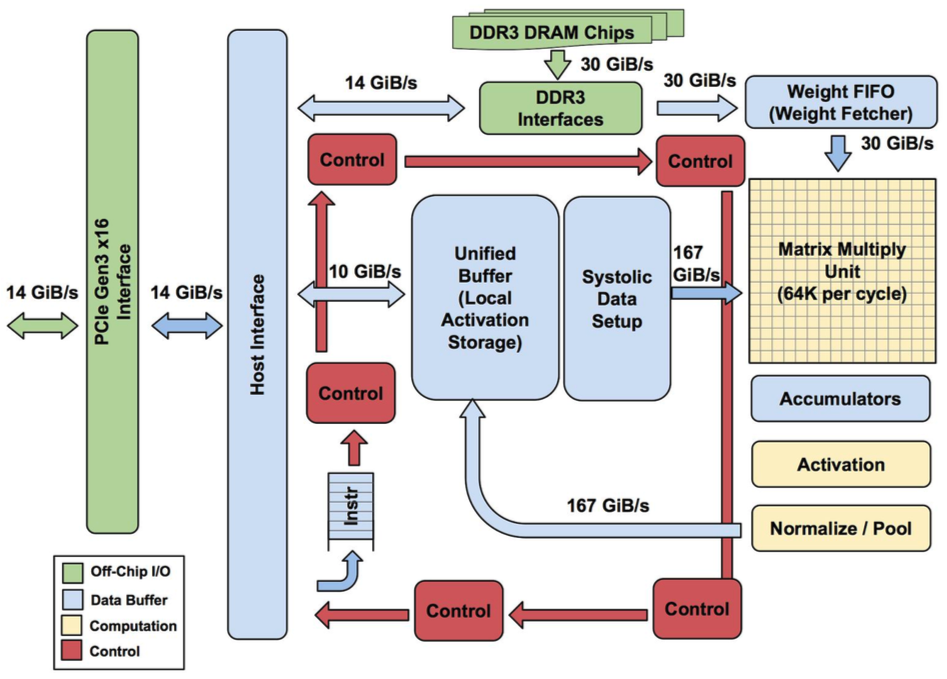
\includegraphics[width=12.5cm, height=10cm]{Bilder/tpu}		
		\caption{Architektur einer Tensor Processing Unit Design \cite{8192463}} 
		\label{fig:TPU}
	\end{figure}
	
	
	

	In dem TPU-Blockdiagramm befindet sich die Matrix-Multiplikationseinheit auf der rechten Seite. Seine Eingänge sind FIFO-Gewichten und der Unified Buffer (UB) und Ausgänge ist der Akkumulator (ACC). Der gelbe Bereich Aktivierung führt die nichtlinearen Funktionen aus und sendet über BUS-Leitung zu Unified Buffer UB.
	Es ist hier bemerkenswert, dass die Bandbreite von Unified Puffer (UB) zur MM-Einheit ist viel höher als die Bandbreite des Puffers von Gewichten, da die Gewichte viel seltener gelesen werden.\\
	Das Herz des TPUs ist die Matrix-Multiplikationseinheit und enthält 256 x 256 MAC (Multiply-Acumulate). Die MACs können 8-Bit-Multiplikationen und Additionen von positiven und negativen Ganzzahlen ausführen.
	\newpage
	Die Gewichte werden zuerst vorgeladen und die Aktivierungen aus dem Aktivierungsspeicherpuffer werden in die MM-Einheit eingelesen. Die Aktivierungen bewegen sich von links nach rechts systolisch und die Teilsummen bewegen sich vertikal von oben nach unten.
	\begin{center}
		
		
	\end{center}

	\begin{figure}[h!]
		\centering
		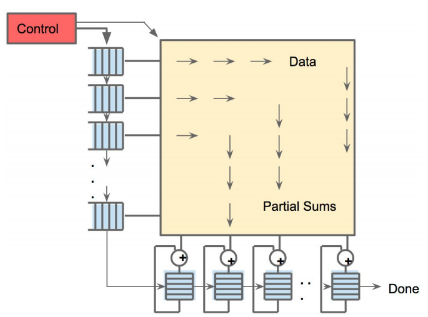
\includegraphics[width=12.5cm, height=10cm]{Bilder/tpusystolic}	
		\caption{Systolischer Datenfluss der Matrix Multiply Unit. Die Gesamtsumme werden in den Akkumulatoren gebildet. \cite{8192463}} 
		\label{fig:sysdaten}
	\end{figure}

	\begin{description}
		\item[\textbf{Systolic Data Setup:}] Hier werden die Daten aus dem Unified Buffer so eingespeist, sodass die Eingänge jeder Zeile um einen Takt zur vorherigen Zeile verzögert werden. Dadurch entsteht eine Latenz von 256-Taktzyklen.
		\item[\textbf{Akkumulatoren:}] In MM-Einheit in MACs finden 8-Bit-Multiplikationen statt und das Ergebnis ist 16-Bit-Produkte. Die werden in den Akkumulator gesammelt und die Teilsumme dazu addiert. Es werden pro Taktzyklus 256 Teilsumme gebildet. Die hier verwendete Akkumulatoren sind 32-Bit Akkumulator und befindet sich unter der MM-Einheit. 
		\item[\textbf{Aktivierung:}] hier werden die Funktionen des künstlichen Neuronen wie Sigmoid, ReLu, usw. ausgeführt. Es kann auch hier die Pooling Operationen \autoref{fig:pooling_layer} für Faltungen ausgeführt werden.

	
	\begin{figure}[h!]
		\centering
		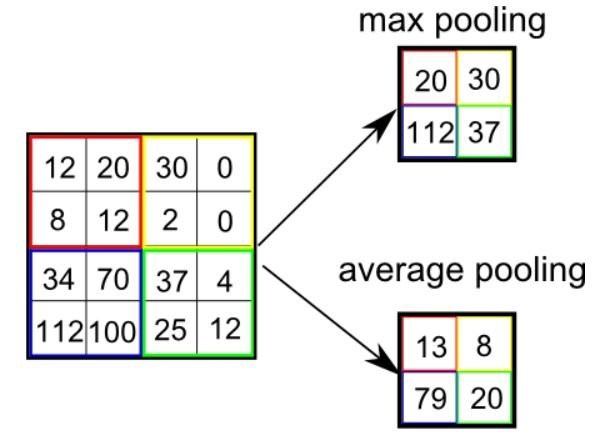
\includegraphics[width=7 cm , height=5 cm]{Bilder/pooling}
		\caption[Pooling]{Average und Max - Pooling}
		\label{fig:pooling_layer}			
	\end{figure}
		
		\item[\textbf{Read\_Host\_Memory:}] liest Daten aus dem CPU\_Hostspeicher in den Unified Buffer (UB).
		\item[\textbf{Read\_Weights:}] liest Gewichte aus dem Gewichtsspeicher-FIFO (Weight-Memory) und im Gewichtsspeicher in die MM-Einheit als Eingabe bereit gestellt.
		\item[\textbf{MatrixMultiply/Convolve:}] mit den geladenen Gewichten und Daten aus dem Unified Buffer wird in MM-Einheit eine Matrixmultiplikation oder eine Faltung ausgeführt werden. Hier kann die eingegebene Matrix variabel sein. Die Matrix mit der Dimension B*256 wird in MM-Einheit mit den geladenen Gewichten 256*256 multipliziert werden. Die Ausgabe kann dann mit der Größe von B*256 in den Akkumulator gespeichert werden, wobei B Pipeline-Zyklen abgeschlossen werden. 
		%\item[\textbf{Activate:}]
		\item[\textbf{Write\_Host\_Memory:}] schreibt Daten aus dem Unified Buffer in den CPU-Hostspeicher und andere Anweisungen sind: alternate host memory read/write, set configuration, zwei Versionen der Synchronisierung, Interrupt-Host, debug-tag, nop und halt.
		%\item[\textbf{Steuerwerke:}]
		%\item[\textbf{Host-Interface:}]
	\end{description}

	\subsection{Vorteile des Systolic Arrays}
	Der Hauptvorteil des TPUs mit Systolic Array Architektur ist seine Unkompliziertheit und es ist nur konzentriert auf Matrix Multiplikation.
	Das TPU Design \autoref{fig:tpudesign} ist einfach und der Stromverbrauch ist gering gehalten. Unified Buffer und MM-Einheit nimmt die maximale Fläche in dem Chip. Die Control Unit nimmt die geringste Fläche, wobei die sehr schwer zu designen war. 
	
	\begin{figure}[h!]
		\centering
		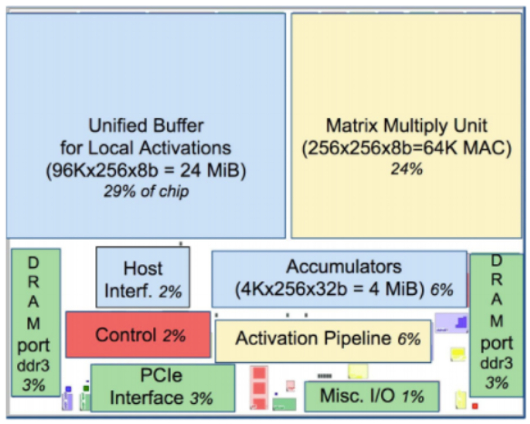
\includegraphics[width=10cm, height=7cm]{Bilder/tpudesign}
		\caption[TPU-Design]{Diese Tabelle zeigt ein Vergleich mit anderen ähnlichen Produkten und der Stromverbrauch ist deutlich geringer als die anderen Geräten.}
		\label{fig:tpudesign}			
	\end{figure}

	\begin{figure}[h!]
		\centering
		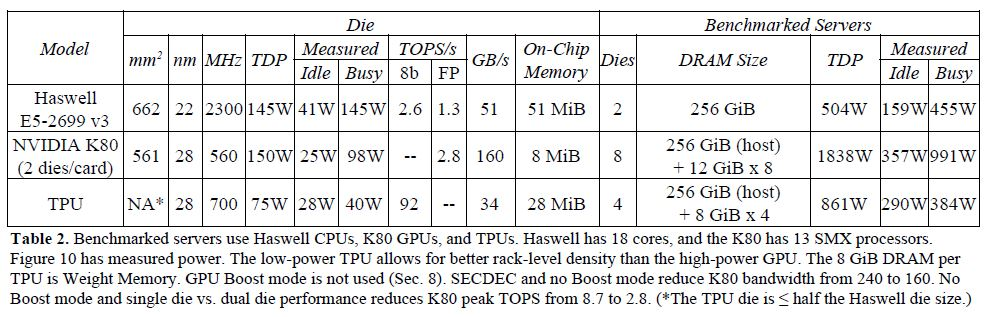
\includegraphics[width=12.5cm, height=5cm]{Bilder/tpuverbrauch}	
		\caption[TPU-Verbrauch]{Diese Tabelle zeigt ein Vergleich mit anderen ähnlichen Produkten und der Stromverbrauch von TPU ist deutlich geringer als die anderen Geräten.}
		\label{fig:tpuverbrauch}			
	\end{figure}

	\subsection{Nachteile des Systolic Arrays}
	Die Multiplikation aus 2 Matrizen N x N dauert 2*N-1 Taktzyklen. Für einen Batch der Größe B beträgt dann die Latenz N*(B+1)-1 . Die Latenz hängt von den Matrixdimensionen ab. Das ist für Anwendungen mit konstanter Latenz nicht wünschenswert.\\
	Ein anderes Problem ist, dass die Eingangsmatrix nicht ein Vielfaches von der PE-Array bzw. MACs in MM-Einheit ist. Bei so einem Fall werden nicht alle verfügbaren MACs verwendet und entsteht damit ungenutzte bzw. verschwendeter Arbeitsspeicher bei nicht standardmäßige Matrixdimensionen.\\
	TPU ist allgemein für Matrixmultiplikationen besser geeignet als Faltungsberechnungen. Die Faltung Operationen können auch ausgeführt werden, indem sie in Matrixmultiplikationen umgewandelt werden. Das ist für große Faltungskerngrößen nicht optimal, da Faltungen spezifische Datenflussmuster aufweisen sollen.Ein gutes Beispiel ist der  Eyeriss-Beschleuniger \textbf{(An Energy-Efficient Reconfigurable Accelerator for Deep Convolutional Neural Networks)}, der speziell für die Faltungsoperation entwickelt wurde.

    \chapter{Implementierung}
    \label{ch:implementierung} 
    \section{Implementierungsplan} Vorgehensweise
    Zur Realisierung der Systolic Array Architektur wird die Programmiersprache VHDL genutzt. 
    Das Kürzel VHDL setzt sich zusammen aus: V steht für VHSIC (\textbf{V}ery \textbf{H}igh \textbf{S}peed \textbf{I}ntegrated \textbf{C}ircuit) und HDL (\textbf{H}ardware \textbf{D}escription \textbf{L}anguage),die im Auftrag der US-Regierung anfangs der 80er entwickelt. Systolic Array Architektur besteht aus RAM (\textbf{R}andom-\textbf{A}ccess \textbf{M}emory), MACs, in dem mehrere Processing Elemente stehen und Delay Control. \autoref{fig:ubersicht} Außerhalb der Block befindet sich ein  Clockgenerator, der mit konstanten Frequenz takten soll.
    

\begin{figure}[h!]
	\centering
		% Graphic for TeX using PGF
% Title: C:\Users\Ahmet\Desktop\BachelorArbeit\ausarbeitung_tex_kit_2016\Ausarbeitung_TeX_KIT\designs\Desing3\Diagramm3.dia
% Creator: Dia v0.97.2
% CreationDate: Thu Feb 13 12:45:10 2020
% For: Ahmet
% \usepackage{tikz}
% The following commands are not supported in PSTricks at present
% We define them conditionally, so when they are implemented,
% this pgf file will use them.
\ifx\du\undefined
  \newlength{\du}
\fi
\setlength{\du}{15\unitlength}
\begin{tikzpicture}
\pgftransformxscale{1.000000}
\pgftransformyscale{-1.000000}
\definecolor{dialinecolor}{rgb}{0.000000, 0.000000, 0.000000}
\pgfsetstrokecolor{dialinecolor}
\definecolor{dialinecolor}{rgb}{1.000000, 1.000000, 1.000000}
\pgfsetfillcolor{dialinecolor}
\pgfsetlinewidth{0.050000\du}
\pgfsetdash{}{0pt}
\pgfsetdash{}{0pt}
\pgfsetmiterjoin
\definecolor{dialinecolor}{rgb}{1.000000, 1.000000, 1.000000}
\pgfsetfillcolor{dialinecolor}
\fill (-2.820630\du,17.468500\du)--(-2.820630\du,19.707697\du)--(2.925874\du,19.707697\du)--(2.925874\du,17.468500\du)--cycle;
\definecolor{dialinecolor}{rgb}{0.000000, 0.000000, 0.000000}
\pgfsetstrokecolor{dialinecolor}
\draw (-2.820630\du,17.468500\du)--(-2.820630\du,19.707697\du)--(2.925874\du,19.707697\du)--(2.925874\du,17.468500\du)--cycle;
% setfont left to latex
\definecolor{dialinecolor}{rgb}{0.000000, 0.000000, 0.000000}
\pgfsetstrokecolor{dialinecolor}
\node at (0.052621\du,18.588100\du){RAM};
\pgfsetlinewidth{0.050000\du}
\pgfsetdash{}{0pt}
\pgfsetdash{}{0pt}
\pgfsetmiterjoin
\definecolor{dialinecolor}{rgb}{1.000000, 1.000000, 1.000000}
\pgfsetfillcolor{dialinecolor}
\fill (8.601110\du,17.471500\du)--(8.601110\du,19.710697\du)--(14.347614\du,19.710697\du)--(14.347614\du,17.471500\du)--cycle;
\definecolor{dialinecolor}{rgb}{0.000000, 0.000000, 0.000000}
\pgfsetstrokecolor{dialinecolor}
\draw (8.601110\du,17.471500\du)--(8.601110\du,19.710697\du)--(14.347614\du,19.710697\du)--(14.347614\du,17.471500\du)--cycle;
% setfont left to latex
\definecolor{dialinecolor}{rgb}{0.000000, 0.000000, 0.000000}
\pgfsetstrokecolor{dialinecolor}
\node at (11.474400\du,18.591100\du){PEs-Array};
\pgfsetlinewidth{0.050000\du}
\pgfsetdash{}{0pt}
\pgfsetdash{}{0pt}
\pgfsetmiterjoin
\definecolor{dialinecolor}{rgb}{1.000000, 1.000000, 1.000000}
\pgfsetfillcolor{dialinecolor}
\fill (8.588560\du,12.152900\du)--(8.588560\du,14.392097\du)--(14.335064\du,14.392097\du)--(14.335064\du,12.152900\du)--cycle;
\definecolor{dialinecolor}{rgb}{0.000000, 0.000000, 0.000000}
\pgfsetstrokecolor{dialinecolor}
\draw (8.588560\du,12.152900\du)--(8.588560\du,14.392097\du)--(14.335064\du,14.392097\du)--(14.335064\du,12.152900\du)--cycle;
% setfont left to latex
\definecolor{dialinecolor}{rgb}{0.000000, 0.000000, 0.000000}
\pgfsetstrokecolor{dialinecolor}
\node at (11.461800\du,13.272500\du){Delay Control};
\pgfsetlinewidth{0.150000\du}
\pgfsetdash{}{0pt}
\pgfsetdash{}{0pt}
\pgfsetbuttcap
{
\definecolor{dialinecolor}{rgb}{0.000000, 0.000000, 0.000000}
\pgfsetfillcolor{dialinecolor}
% was here!!!
\pgfsetarrowsend{latex}
\definecolor{dialinecolor}{rgb}{0.000000, 0.000000, 0.000000}
\pgfsetstrokecolor{dialinecolor}
\draw (11.009500\du,17.445800\du)--(11.012200\du,14.434600\du);
}
\pgfsetlinewidth{0.150000\du}
\pgfsetdash{}{0pt}
\pgfsetdash{}{0pt}
\pgfsetbuttcap
{
\definecolor{dialinecolor}{rgb}{0.000000, 0.000000, 0.000000}
\pgfsetfillcolor{dialinecolor}
% was here!!!
\pgfsetarrowsend{latex}
\definecolor{dialinecolor}{rgb}{0.000000, 0.000000, 0.000000}
\pgfsetstrokecolor{dialinecolor}
\draw (12.998100\du,17.459500\du)--(13.000800\du,14.448300\du);
}
\pgfsetlinewidth{0.150000\du}
\pgfsetdash{}{0pt}
\pgfsetdash{}{0pt}
\pgfsetbuttcap
{
\definecolor{dialinecolor}{rgb}{0.000000, 0.000000, 0.000000}
\pgfsetfillcolor{dialinecolor}
% was here!!!
\pgfsetarrowsend{latex}
\definecolor{dialinecolor}{rgb}{0.000000, 0.000000, 0.000000}
\pgfsetstrokecolor{dialinecolor}
\draw (10.015300\du,17.439000\du)--(10.017900\du,14.427800\du);
}
\pgfsetlinewidth{0.150000\du}
\pgfsetdash{}{0pt}
\pgfsetdash{}{0pt}
\pgfsetbuttcap
{
\definecolor{dialinecolor}{rgb}{0.000000, 0.000000, 0.000000}
\pgfsetfillcolor{dialinecolor}
% was here!!!
\pgfsetarrowsend{latex}
\definecolor{dialinecolor}{rgb}{0.000000, 0.000000, 0.000000}
\pgfsetstrokecolor{dialinecolor}
\draw (12.018000\du,17.442400\du)--(12.020700\du,14.431200\du);
}
\pgfsetlinewidth{0.150000\du}
\pgfsetdash{}{0pt}
\pgfsetdash{}{0pt}
\pgfsetbuttcap
{
\definecolor{dialinecolor}{rgb}{0.000000, 0.000000, 1.000000}
\pgfsetfillcolor{dialinecolor}
% was here!!!
\pgfsetarrowsend{latex}
\definecolor{dialinecolor}{rgb}{0.000000, 0.000000, 1.000000}
\pgfsetstrokecolor{dialinecolor}
\draw (2.925870\du,18.050300\du)--(8.601110\du,18.053400\du);
}
\pgfsetlinewidth{0.150000\du}
\pgfsetdash{}{0pt}
\pgfsetdash{}{0pt}
\pgfsetbuttcap
{
\definecolor{dialinecolor}{rgb}{1.000000, 0.000000, 0.000000}
\pgfsetfillcolor{dialinecolor}
% was here!!!
\pgfsetarrowsend{latex}
\definecolor{dialinecolor}{rgb}{1.000000, 0.000000, 0.000000}
\pgfsetstrokecolor{dialinecolor}
\draw (2.897470\du,18.973800\du)--(8.572710\du,18.976900\du);
}
% setfont left to latex
\definecolor{dialinecolor}{rgb}{0.000000, 0.000000, 0.000000}
\pgfsetstrokecolor{dialinecolor}
\node at (6.130760\du,17.658800\du){MatrixA};
% setfont left to latex
\definecolor{dialinecolor}{rgb}{0.000000, 0.000000, 0.000000}
\pgfsetstrokecolor{dialinecolor}
\node at (6.215380\du,19.719600\du){MatrixB};
\pgfsetlinewidth{0.150000\du}
\pgfsetdash{}{0pt}
\pgfsetdash{}{0pt}
\pgfsetmiterjoin
\pgfsetbuttcap
{
\definecolor{dialinecolor}{rgb}{0.000000, 1.000000, 0.000000}
\pgfsetfillcolor{dialinecolor}
% was here!!!
\pgfsetarrowsend{latex}
{\pgfsetcornersarced{\pgfpoint{0.000000\du}{0.000000\du}}\definecolor{dialinecolor}{rgb}{0.000000, 1.000000, 0.000000}
\pgfsetstrokecolor{dialinecolor}
\draw (8.588560\du,13.272498\du)--(0.052622\du,13.272498\du)--(0.052622\du,17.468500\du);
}}
% setfont left to latex
\definecolor{dialinecolor}{rgb}{0.000000, 0.000000, 0.000000}
\pgfsetstrokecolor{dialinecolor}
\node at (1.135530\du,12.260100\du){Completed C's};
% setfont left to latex
\definecolor{dialinecolor}{rgb}{0.000000, 0.000000, 0.000000}
\pgfsetstrokecolor{dialinecolor}
\node at (1.135530\du,13.060100\du){with delays};
% setfont left to latex
\definecolor{dialinecolor}{rgb}{0.000000, 0.000000, 0.000000}
\pgfsetstrokecolor{dialinecolor}
\node at (16.981200\du,15.830200\du){Completed matrix };
% setfont left to latex
\definecolor{dialinecolor}{rgb}{0.000000, 0.000000, 0.000000}
\pgfsetstrokecolor{dialinecolor}
\node at (16.981200\du,16.630200\du){product C };
\pgfsetlinewidth{0.050000\du}
\pgfsetdash{}{0pt}
\pgfsetdash{}{0pt}
\pgfsetbuttcap
\pgfsetmiterjoin
\pgfsetlinewidth{0.050000\du}
\pgfsetbuttcap
\pgfsetmiterjoin
\pgfsetdash{}{0pt}
\definecolor{dialinecolor}{rgb}{1.000000, 1.000000, 1.000000}
\pgfsetfillcolor{dialinecolor}
\fill (-9.352060\du,17.548200\du)--(-9.352060\du,19.548200\du)--(-7.416576\du,19.548200\du)--(-7.416576\du,17.548200\du)--cycle;
\definecolor{dialinecolor}{rgb}{0.000000, 0.000000, 0.000000}
\pgfsetstrokecolor{dialinecolor}
\draw (-9.352060\du,17.548200\du)--(-9.352060\du,19.548200\du)--(-7.416576\du,19.548200\du)--(-7.416576\du,17.548200\du)--cycle;
\pgfsetbuttcap
\pgfsetmiterjoin
\pgfsetdash{}{0pt}
\definecolor{dialinecolor}{rgb}{0.000000, 0.000000, 0.000000}
\pgfsetstrokecolor{dialinecolor}
\draw (-9.352060\du,17.548200\du)--(-9.352060\du,19.548200\du)--(-7.416576\du,19.548200\du)--(-7.416576\du,17.548200\du)--cycle;
% setfont left to latex
\definecolor{dialinecolor}{rgb}{0.000000, 0.000000, 0.000000}
\pgfsetstrokecolor{dialinecolor}
\node at (-8.384320\du,18.548200\du){clk};
\pgfsetlinewidth{0.150000\du}
\pgfsetdash{}{0pt}
\pgfsetdash{}{0pt}
\pgfsetmiterjoin
\pgfsetbuttcap
{
\definecolor{dialinecolor}{rgb}{0.000000, 0.000000, 1.000000}
\pgfsetfillcolor{dialinecolor}
% was here!!!
\pgfsetarrowsend{latex}
{\pgfsetcornersarced{\pgfpoint{0.000000\du}{0.000000\du}}\definecolor{dialinecolor}{rgb}{0.000000, 0.000000, 1.000000}
\pgfsetstrokecolor{dialinecolor}
\draw (-7.416580\du,18.548200\du)--(-6.795200\du,18.548200\du)--(-6.795200\du,8.997660\du)--(11.461800\du,8.997660\du)--(11.461800\du,12.152900\du);
}}
\pgfsetlinewidth{0.150000\du}
\pgfsetdash{}{0pt}
\pgfsetdash{}{0pt}
\pgfsetbuttcap
{
\definecolor{dialinecolor}{rgb}{0.000000, 0.000000, 1.000000}
\pgfsetfillcolor{dialinecolor}
% was here!!!
\pgfsetarrowsend{latex}
\definecolor{dialinecolor}{rgb}{0.000000, 0.000000, 1.000000}
\pgfsetstrokecolor{dialinecolor}
\draw (-7.416580\du,18.548200\du)--(-2.820630\du,18.588100\du);
}
\pgfsetlinewidth{0.150000\du}
\pgfsetdash{}{0pt}
\pgfsetdash{}{0pt}
\pgfsetmiterjoin
\definecolor{dialinecolor}{rgb}{0.000000, 0.000000, 0.000000}
\pgfsetstrokecolor{dialinecolor}
\draw (-3.371987\du,10.975785\du)--(-3.371987\du,21.066356\du)--(20.557083\du,21.066356\du)--(20.557083\du,10.975785\du)--cycle;
\pgfsetlinewidth{0.150000\du}
\pgfsetdash{}{0pt}
\pgfsetdash{}{0pt}
\pgfsetmiterjoin
\pgfsetbuttcap
{
\definecolor{dialinecolor}{rgb}{0.000000, 0.000000, 1.000000}
\pgfsetfillcolor{dialinecolor}
% was here!!!
\pgfsetarrowsend{latex}
{\pgfsetcornersarced{\pgfpoint{0.000000\du}{0.000000\du}}\definecolor{dialinecolor}{rgb}{0.000000, 0.000000, 1.000000}
\pgfsetstrokecolor{dialinecolor}
\draw (-7.416576\du,18.548200\du)--(-5.394282\du,18.548200\du)--(-5.394282\du,16.021070\du)--(-3.371987\du,16.021070\du);
}}
% setfont left to latex
\definecolor{dialinecolor}{rgb}{0.000000, 0.000000, 0.000000}
\pgfsetstrokecolor{dialinecolor}
\node at (7.682540\du,8.305740\du){Control Matrix Multiplier};
\pgfsetlinewidth{0.150000\du}
\pgfsetdash{}{0pt}
\pgfsetdash{}{0pt}
\pgfsetmiterjoin
\pgfsetbuttcap
{
\definecolor{dialinecolor}{rgb}{0.000000, 0.000000, 1.000000}
\pgfsetfillcolor{dialinecolor}
% was here!!!
\pgfsetarrowsend{latex}
{\pgfsetcornersarced{\pgfpoint{0.000000\du}{0.000000\du}}\definecolor{dialinecolor}{rgb}{0.000000, 0.000000, 1.000000}
\pgfsetstrokecolor{dialinecolor}
\draw (-7.416580\du,18.548200\du)--(-6.790230\du,18.548200\du)--(-6.790230\du,22.086600\du)--(11.474400\du,22.086600\du)--(11.474400\du,19.710700\du);
}}
\end{tikzpicture}

	\caption{ Übersicht des Codes für die Matrixmultiplikation}
	\label{fig:ubersicht}
\end{figure}

	\subsection{MAC}\label{subsec:MAC}
	In dem Block MACs befinden mehrere PE (Processing Elements) und sie sind miteinander verbunden, sodass die Daten systolisch durch die Elemente bewegen. Ein PE hat zwei Eingänge und zwei enable Signale. Es findet die Berechnung dann statt, wenn enable Signale auf HIGH gesetz sind. Das Ergebnis wird in dem Akkumulator von PE zur Teilsumme addiert. Dabei wird die Berechnungen durch ein Zähler bis zu einem bestimmten Wert gezählt. Wenn der Zähler fertig ist, dann wird die Gesamtsumme zum Speicher gesendet.
	 \begin{center}
		% Graphic for TeX using PGF
% Title: C:\Users\Ahmet\Desktop\BachelorArbeit\ausarbeitung_tex_kit_2016\Ausarbeitung_TeX_KIT\designs\Design4\Diagramm4.dia
% Creator: Dia v0.97.2
% CreationDate: Mon Jan 20 00:31:43 2020
% For: Ahmet
% \usepackage{tikz}
% The following commands are not supported in PSTricks at present
% We define them conditionally, so when they are implemented,
% this pgf file will use them.
\ifx\du\undefined
  \newlength{\du}
\fi
\setlength{\du}{15\unitlength}
\begin{tikzpicture}
\pgftransformxscale{1.000000}
\pgftransformyscale{-1.000000}
\definecolor{dialinecolor}{rgb}{0.000000, 0.000000, 0.000000}
\pgfsetstrokecolor{dialinecolor}
\definecolor{dialinecolor}{rgb}{1.000000, 1.000000, 1.000000}
\pgfsetfillcolor{dialinecolor}
\pgfsetlinewidth{0.050000\du}
\pgfsetdash{}{0pt}
\pgfsetdash{}{0pt}
\pgfsetbuttcap
\pgfsetmiterjoin
\pgfsetlinewidth{0.050000\du}
\pgfsetbuttcap
\pgfsetmiterjoin
\pgfsetdash{}{0pt}
\definecolor{dialinecolor}{rgb}{1.000000, 1.000000, 1.000000}
\pgfsetfillcolor{dialinecolor}
\fill (25.982258\du,13.850000\du)--(25.982258\du,15.515000\du)--(27.593548\du,15.515000\du)--(27.593548\du,13.850000\du)--cycle;
\definecolor{dialinecolor}{rgb}{0.000000, 0.000000, 0.000000}
\pgfsetstrokecolor{dialinecolor}
\draw (25.982258\du,13.850000\du)--(25.982258\du,15.515000\du)--(27.593548\du,15.515000\du)--(27.593548\du,13.850000\du)--cycle;
\pgfsetbuttcap
\pgfsetmiterjoin
\pgfsetdash{}{0pt}
\definecolor{dialinecolor}{rgb}{0.000000, 0.000000, 0.000000}
\pgfsetstrokecolor{dialinecolor}
\draw (25.982258\du,13.850000\du)--(25.982258\du,15.515000\du)--(27.593548\du,15.515000\du)--(27.593548\du,13.850000\du)--cycle;
% setfont left to latex
\definecolor{dialinecolor}{rgb}{0.000000, 0.000000, 0.000000}
\pgfsetstrokecolor{dialinecolor}
\node at (26.787903\du,14.682500\du){X};
\pgfsetlinewidth{0.050000\du}
\pgfsetdash{}{0pt}
\pgfsetdash{}{0pt}
\pgfsetmiterjoin
\definecolor{dialinecolor}{rgb}{1.000000, 1.000000, 1.000000}
\pgfsetfillcolor{dialinecolor}
\fill (21.485429\du,16.592897\du)--(21.485429\du,17.603720\du)--(25.736831\du,17.603720\du)--(25.736831\du,16.592897\du)--cycle;
\definecolor{dialinecolor}{rgb}{0.000000, 0.000000, 0.000000}
\pgfsetstrokecolor{dialinecolor}
\draw (21.485429\du,16.592897\du)--(21.485429\du,17.603720\du)--(25.736831\du,17.603720\du)--(25.736831\du,16.592897\du)--cycle;
% setfont left to latex
\definecolor{dialinecolor}{rgb}{0.000000, 0.000000, 0.000000}
\pgfsetstrokecolor{dialinecolor}
\node[anchor=west] at (23.611130\du,17.098309\du){};
% setfont left to latex
\definecolor{dialinecolor}{rgb}{0.000000, 0.000000, 0.000000}
\pgfsetstrokecolor{dialinecolor}
\node at (23.611130\du,17.098309\du){Register};
\pgfsetlinewidth{0.050000\du}
\pgfsetdash{}{0pt}
\pgfsetdash{}{0pt}
\pgfsetmiterjoin
\definecolor{dialinecolor}{rgb}{1.000000, 1.000000, 1.000000}
\pgfsetfillcolor{dialinecolor}
\fill (28.834822\du,12.121318\du)--(28.834822\du,13.132140\du)--(33.086224\du,13.132140\du)--(33.086224\du,12.121318\du)--cycle;
\definecolor{dialinecolor}{rgb}{0.000000, 0.000000, 0.000000}
\pgfsetstrokecolor{dialinecolor}
\draw (28.834822\du,12.121318\du)--(28.834822\du,13.132140\du)--(33.086224\du,13.132140\du)--(33.086224\du,12.121318\du)--cycle;
% setfont left to latex
\definecolor{dialinecolor}{rgb}{0.000000, 0.000000, 0.000000}
\pgfsetstrokecolor{dialinecolor}
\node[anchor=west] at (30.960523\du,12.626729\du){};
% setfont left to latex
\definecolor{dialinecolor}{rgb}{0.000000, 0.000000, 0.000000}
\pgfsetstrokecolor{dialinecolor}
\node at (30.960523\du,12.626729\du){Register};
\pgfsetlinewidth{0.050000\du}
\pgfsetdash{}{0pt}
\pgfsetdash{}{0pt}
\pgfsetbuttcap
{
\definecolor{dialinecolor}{rgb}{0.000000, 0.000000, 0.000000}
\pgfsetfillcolor{dialinecolor}
% was here!!!
\pgfsetarrowsend{latex}
\definecolor{dialinecolor}{rgb}{0.000000, 0.000000, 0.000000}
\pgfsetstrokecolor{dialinecolor}
\draw (26.788554\du,9.240561\du)--(26.787903\du,13.850000\du);
}
\pgfsetlinewidth{0.050000\du}
\pgfsetdash{}{0pt}
\pgfsetdash{}{0pt}
\pgfsetmiterjoin
\pgfsetbuttcap
{
\definecolor{dialinecolor}{rgb}{0.000000, 0.000000, 0.000000}
\pgfsetfillcolor{dialinecolor}
% was here!!!
\pgfsetarrowsend{latex}
{\pgfsetcornersarced{\pgfpoint{0.000000\du}{0.000000\du}}\definecolor{dialinecolor}{rgb}{0.000000, 0.000000, 0.000000}
\pgfsetstrokecolor{dialinecolor}
\draw (26.788228\du,11.545281\du)--(23.611130\du,11.545281\du)--(23.611130\du,16.592897\du);
}}
\pgfsetlinewidth{0.050000\du}
\pgfsetdash{}{0pt}
\pgfsetdash{}{0pt}
\pgfsetbuttcap
{
\definecolor{dialinecolor}{rgb}{0.000000, 0.000000, 0.000000}
\pgfsetfillcolor{dialinecolor}
% was here!!!
\pgfsetarrowsend{latex}
\definecolor{dialinecolor}{rgb}{0.000000, 0.000000, 0.000000}
\pgfsetstrokecolor{dialinecolor}
\draw (18.988577\du,14.690545\du)--(25.982258\du,14.682500\du);
}
\pgfsetlinewidth{0.050000\du}
\pgfsetdash{}{0pt}
\pgfsetdash{}{0pt}
\pgfsetmiterjoin
\definecolor{dialinecolor}{rgb}{1.000000, 1.000000, 1.000000}
\pgfsetfillcolor{dialinecolor}
\fill (28.563548\du,16.660539\du)--(28.563548\du,17.671362\du)--(31.438540\du,17.671362\du)--(31.438540\du,16.660539\du)--cycle;
\definecolor{dialinecolor}{rgb}{0.000000, 0.000000, 0.000000}
\pgfsetstrokecolor{dialinecolor}
\draw (28.563548\du,16.660539\du)--(28.563548\du,17.671362\du)--(31.438540\du,17.671362\du)--(31.438540\du,16.660539\du)--cycle;
% setfont left to latex
\definecolor{dialinecolor}{rgb}{0.000000, 0.000000, 0.000000}
\pgfsetstrokecolor{dialinecolor}
\node at (30.001044\du,17.165951\du){acc};
\pgfsetlinewidth{0.050000\du}
\pgfsetdash{}{0pt}
\pgfsetdash{}{0pt}
\pgfsetmiterjoin
\pgfsetbuttcap
{
\definecolor{dialinecolor}{rgb}{0.000000, 0.000000, 0.000000}
\pgfsetfillcolor{dialinecolor}
% was here!!!
\pgfsetarrowsend{latex}
{\pgfsetcornersarced{\pgfpoint{0.000000\du}{0.000000\du}}\definecolor{dialinecolor}{rgb}{0.000000, 0.000000, 0.000000}
\pgfsetstrokecolor{dialinecolor}
\draw (26.787903\du,15.515000\du)--(26.787903\du,16.087770\du)--(30.001044\du,16.087770\du)--(30.001044\du,16.660539\du);
}}
\pgfsetlinewidth{0.050000\du}
\pgfsetdash{}{0pt}
\pgfsetdash{}{0pt}
\pgfsetbuttcap
{
\definecolor{dialinecolor}{rgb}{0.000000, 0.000000, 0.000000}
\pgfsetfillcolor{dialinecolor}
% was here!!!
\pgfsetarrowsend{latex}
\definecolor{dialinecolor}{rgb}{0.000000, 0.000000, 0.000000}
\pgfsetstrokecolor{dialinecolor}
\draw (30.001044\du,17.671362\du)--(29.988544\du,20.940527\du);
}
\pgfsetlinewidth{0.050000\du}
\pgfsetdash{}{0pt}
\pgfsetdash{}{0pt}
\pgfsetmiterjoin
\pgfsetbuttcap
{
\definecolor{dialinecolor}{rgb}{0.000000, 0.000000, 0.000000}
\pgfsetfillcolor{dialinecolor}
% was here!!!
\pgfsetarrowsend{latex}
{\pgfsetcornersarced{\pgfpoint{0.000000\du}{0.000000\du}}\definecolor{dialinecolor}{rgb}{0.000000, 0.000000, 0.000000}
\pgfsetstrokecolor{dialinecolor}
\draw (30.688542\du,17.740536\du)--(30.688542\du,18.340534\du)--(32.138538\du,18.340534\du)--(32.138538\du,15.640542\du)--(30.738542\du,15.640542\du)--(30.738542\du,16.590540\du);
}}
\pgfsetlinewidth{0.050000\du}
\pgfsetdash{}{0pt}
\pgfsetdash{}{0pt}
\pgfsetmiterjoin
\pgfsetbuttcap
{
\definecolor{dialinecolor}{rgb}{0.000000, 0.000000, 0.000000}
\pgfsetfillcolor{dialinecolor}
% was here!!!
\pgfsetarrowsend{latex}
{\pgfsetcornersarced{\pgfpoint{0.000000\du}{0.000000\du}}\definecolor{dialinecolor}{rgb}{0.000000, 0.000000, 0.000000}
\pgfsetstrokecolor{dialinecolor}
\draw (22.485417\du,14.686523\du)--(22.485417\du,12.626729\du)--(28.834822\du,12.626729\du);
}}
\pgfsetlinewidth{0.050000\du}
\pgfsetdash{}{0pt}
\pgfsetdash{}{0pt}
\pgfsetbuttcap
{
\definecolor{dialinecolor}{rgb}{0.000000, 0.000000, 0.000000}
\pgfsetfillcolor{dialinecolor}
% was here!!!
\pgfsetarrowsend{latex}
\definecolor{dialinecolor}{rgb}{0.000000, 0.000000, 0.000000}
\pgfsetstrokecolor{dialinecolor}
\draw (33.086224\du,12.626729\du)--(37.338522\du,12.640551\du);
}
\pgfsetlinewidth{0.050000\du}
\pgfsetdash{}{0pt}
\pgfsetdash{}{0pt}
\pgfsetmiterjoin
\pgfsetbuttcap
{
\definecolor{dialinecolor}{rgb}{0.000000, 0.000000, 0.000000}
\pgfsetfillcolor{dialinecolor}
% was here!!!
\pgfsetarrowsend{latex}
{\pgfsetcornersarced{\pgfpoint{0.000000\du}{0.000000\du}}\definecolor{dialinecolor}{rgb}{0.000000, 0.000000, 0.000000}
\pgfsetstrokecolor{dialinecolor}
\draw (23.611130\du,17.603720\du)--(23.611130\du,19.347123\du)--(27.038553\du,19.347123\du)--(27.038553\du,21.090526\du);
}}
% setfont left to latex
\definecolor{dialinecolor}{rgb}{0.000000, 0.000000, 0.000000}
\pgfsetstrokecolor{dialinecolor}
\node at (27.438552\du,9.740560\du){bi};
% setfont left to latex
\definecolor{dialinecolor}{rgb}{0.000000, 0.000000, 0.000000}
\pgfsetstrokecolor{dialinecolor}
\node at (19.288576\du,14.290546\du){ai};
\pgfsetlinewidth{0.050000\du}
\pgfsetdash{}{0pt}
\pgfsetdash{}{0pt}
\pgfsetmiterjoin
\definecolor{dialinecolor}{rgb}{0.000000, 0.000000, 0.000000}
\pgfsetstrokecolor{dialinecolor}
\draw (20.988571\du,10.090559\du)--(20.988571\du,19.940530\du)--(33.638533\du,19.940530\du)--(33.638533\du,10.090559\du)--cycle;
% setfont left to latex
\definecolor{dialinecolor}{rgb}{0.000000, 0.000000, 0.000000}
\pgfsetstrokecolor{dialinecolor}
\node at (26.338555\du,20.640528\du){bi};
% setfont left to latex
\definecolor{dialinecolor}{rgb}{0.000000, 0.000000, 0.000000}
\pgfsetstrokecolor{dialinecolor}
\node at (31.938538\du,20.690527\du){result\_out};
% setfont left to latex
\definecolor{dialinecolor}{rgb}{0.000000, 0.000000, 0.000000}
\pgfsetstrokecolor{dialinecolor}
\node at (36.288525\du,12.290552\du){ai};
% setfont left to latex
\definecolor{dialinecolor}{rgb}{0.000000, 0.000000, 0.000000}
\pgfsetstrokecolor{dialinecolor}
\node at (27.188552\du,7.940565\du){Procossing Element};
\end{tikzpicture}

	\end{center}

	\subsection{RAM} \label{subsec:RAM}
	In RAM werden die Eingangsmatrizen A-und B-Matrix gespeichert und fließen die Matrixelemente in die PE rein. Damit die richtige Matrixelemente in die richtige PE fließen kann, wird hier die logische Signale wie A\_enable und B\_enable genutzt.
	
	% BUraya bidaha bak yazmadan önce!!
	A\_enable bzw. B\_enable sind 3 Bit groß und wird im VHDL-Code so angewendet.\\
	Wenn A\_enable := 001 und A\_enable := 001 sind, dann werden nur die erste Zeile von Matrizen eingespeist und in PE berechnet. Nachdem alle Elemente aus der ersten Zeile eingespeist sind dann werden die  A\_enable := 010 und A\_enable := 010, um die zweite Zeile zu berechnen usw.
	
	\subsection{Delay Controller}
	Innerhalb der MACs-Komponente in Register von PEs werden die Teilsumme zur Gesamtsumme akkumuliert, sobald die Gesamtsumme bereit sind, werden sie dann zu Delay Controller gesendet. Jede Elemente der Produktmatrix hat eigenen Eingang und die Elemente werden dann zu RAM Adresse zugewiesen. Innerhalb der Delay Controller werden dann jede Elemente von Produktmatrix verzögert abgebildet und zum RAM zum speichern gesendet.

	\subsection{Register in MAC} 
	Die Register Blöcke verzögern die Daten für einen Taktzyklus. Dies ist entscheidend für die Implementierung des systolischen Architektur. Ohne die Register wäre es nicht möglich den Datenfluss in MM-Unit zu kontrollieren.
	\begin{center}
		% Graphic for TeX using PGF
% Title: C:\Users\Ahmet\Desktop\BachelorArbeit\ausarbeitung_tex_kit_2016\Ausarbeitung_TeX_KIT\designs\design5\Diagramm5.dia
% Creator: Dia v0.97.2
% CreationDate: Mon Jan 20 02:07:35 2020
% For: Ahmet
% \usepackage{tikz}
% The following commands are not supported in PSTricks at present
% We define them conditionally, so when they are implemented,
% this pgf file will use them.
\ifx\du\undefined
  \newlength{\du}
\fi
\setlength{\du}{15\unitlength}
\begin{tikzpicture}
\pgftransformxscale{1.000000}
\pgftransformyscale{-1.000000}
\definecolor{dialinecolor}{rgb}{0.000000, 0.000000, 0.000000}
\pgfsetstrokecolor{dialinecolor}
\definecolor{dialinecolor}{rgb}{1.000000, 1.000000, 1.000000}
\pgfsetfillcolor{dialinecolor}
\pgfsetlinewidth{0.050000\du}
\pgfsetdash{}{0pt}
\pgfsetdash{}{0pt}
\pgfsetmiterjoin
\definecolor{dialinecolor}{rgb}{1.000000, 1.000000, 1.000000}
\pgfsetfillcolor{dialinecolor}
\fill (8.500000\du,7.013067\du)--(8.500000\du,8.113067\du)--(11.650000\du,8.113067\du)--(11.650000\du,7.013067\du)--cycle;
\definecolor{dialinecolor}{rgb}{0.000000, 0.000000, 0.000000}
\pgfsetstrokecolor{dialinecolor}
\draw (8.500000\du,7.013067\du)--(8.500000\du,8.113067\du)--(11.650000\du,8.113067\du)--(11.650000\du,7.013067\du)--cycle;
\pgfsetlinewidth{0.050000\du}
\pgfsetdash{}{0pt}
\pgfsetdash{}{0pt}
\pgfsetbuttcap
\pgfsetmiterjoin
\pgfsetlinewidth{0.050000\du}
\pgfsetbuttcap
\pgfsetmiterjoin
\pgfsetdash{}{0pt}
\definecolor{dialinecolor}{rgb}{1.000000, 1.000000, 1.000000}
\pgfsetfillcolor{dialinecolor}
\fill (5.232258\du,6.600000\du)--(5.232258\du,8.600000\du)--(7.167742\du,8.600000\du)--(7.167742\du,6.600000\du)--cycle;
\definecolor{dialinecolor}{rgb}{0.000000, 0.000000, 0.000000}
\pgfsetstrokecolor{dialinecolor}
\draw (5.232258\du,6.600000\du)--(5.232258\du,8.600000\du)--(7.167742\du,8.600000\du)--(7.167742\du,6.600000\du)--cycle;
\pgfsetbuttcap
\pgfsetmiterjoin
\pgfsetdash{}{0pt}
\definecolor{dialinecolor}{rgb}{0.000000, 0.000000, 0.000000}
\pgfsetstrokecolor{dialinecolor}
\draw (5.232258\du,6.600000\du)--(5.232258\du,8.600000\du)--(7.167742\du,8.600000\du)--(7.167742\du,6.600000\du)--cycle;
% setfont left to latex
\definecolor{dialinecolor}{rgb}{0.000000, 0.000000, 0.000000}
\pgfsetstrokecolor{dialinecolor}
\node at (6.200000\du,7.600000\du){PE};
% setfont left to latex
\definecolor{dialinecolor}{rgb}{0.000000, 0.000000, 0.000000}
\pgfsetstrokecolor{dialinecolor}
\node at (10.075000\du,7.563067\du){Register};
\pgfsetlinewidth{0.050000\du}
\pgfsetdash{}{0pt}
\pgfsetdash{}{0pt}
\pgfsetbuttcap
{
\definecolor{dialinecolor}{rgb}{0.000000, 0.000000, 0.000000}
\pgfsetfillcolor{dialinecolor}
% was here!!!
\pgfsetarrowsend{latex}
\definecolor{dialinecolor}{rgb}{0.000000, 0.000000, 0.000000}
\pgfsetstrokecolor{dialinecolor}
\draw (7.167742\du,7.600000\du)--(8.402958\du,7.632586\du);
}
\pgfsetlinewidth{0.050000\du}
\pgfsetdash{}{0pt}
\pgfsetdash{}{0pt}
\pgfsetbuttcap
{
\definecolor{dialinecolor}{rgb}{0.000000, 0.000000, 0.000000}
\pgfsetfillcolor{dialinecolor}
% was here!!!
\pgfsetarrowsend{latex}
\definecolor{dialinecolor}{rgb}{0.000000, 0.000000, 0.000000}
\pgfsetstrokecolor{dialinecolor}
\draw (11.650000\du,7.563067\du)--(12.915282\du,7.563199\du);
}
\pgfsetlinewidth{0.050000\du}
\pgfsetdash{}{0pt}
\pgfsetdash{}{0pt}
\pgfsetmiterjoin
\definecolor{dialinecolor}{rgb}{1.000000, 1.000000, 1.000000}
\pgfsetfillcolor{dialinecolor}
\fill (16.168622\du,7.010198\du)--(16.168622\du,8.110198\du)--(19.318622\du,8.110198\du)--(19.318622\du,7.010198\du)--cycle;
\definecolor{dialinecolor}{rgb}{0.000000, 0.000000, 0.000000}
\pgfsetstrokecolor{dialinecolor}
\draw (16.168622\du,7.010198\du)--(16.168622\du,8.110198\du)--(19.318622\du,8.110198\du)--(19.318622\du,7.010198\du)--cycle;
\pgfsetlinewidth{0.050000\du}
\pgfsetdash{}{0pt}
\pgfsetdash{}{0pt}
\pgfsetbuttcap
\pgfsetmiterjoin
\pgfsetlinewidth{0.050000\du}
\pgfsetbuttcap
\pgfsetmiterjoin
\pgfsetdash{}{0pt}
\definecolor{dialinecolor}{rgb}{1.000000, 1.000000, 1.000000}
\pgfsetfillcolor{dialinecolor}
\fill (12.900880\du,6.597131\du)--(12.900880\du,8.597131\du)--(14.836364\du,8.597131\du)--(14.836364\du,6.597131\du)--cycle;
\definecolor{dialinecolor}{rgb}{0.000000, 0.000000, 0.000000}
\pgfsetstrokecolor{dialinecolor}
\draw (12.900880\du,6.597131\du)--(12.900880\du,8.597131\du)--(14.836364\du,8.597131\du)--(14.836364\du,6.597131\du)--cycle;
\pgfsetbuttcap
\pgfsetmiterjoin
\pgfsetdash{}{0pt}
\definecolor{dialinecolor}{rgb}{0.000000, 0.000000, 0.000000}
\pgfsetstrokecolor{dialinecolor}
\draw (12.900880\du,6.597131\du)--(12.900880\du,8.597131\du)--(14.836364\du,8.597131\du)--(14.836364\du,6.597131\du)--cycle;
% setfont left to latex
\definecolor{dialinecolor}{rgb}{0.000000, 0.000000, 0.000000}
\pgfsetstrokecolor{dialinecolor}
\node at (13.868622\du,7.597131\du){PE};
% setfont left to latex
\definecolor{dialinecolor}{rgb}{0.000000, 0.000000, 0.000000}
\pgfsetstrokecolor{dialinecolor}
\node at (17.743622\du,7.560198\du){Register};
\pgfsetlinewidth{0.050000\du}
\pgfsetdash{}{0pt}
\pgfsetdash{}{0pt}
\pgfsetbuttcap
{
\definecolor{dialinecolor}{rgb}{0.000000, 0.000000, 0.000000}
\pgfsetfillcolor{dialinecolor}
% was here!!!
\pgfsetarrowsend{latex}
\definecolor{dialinecolor}{rgb}{0.000000, 0.000000, 0.000000}
\pgfsetstrokecolor{dialinecolor}
\draw (14.836364\du,7.597131\du)--(16.071579\du,7.629717\du);
}
\pgfsetlinewidth{0.050000\du}
\pgfsetdash{}{0pt}
\pgfsetdash{}{0pt}
\pgfsetbuttcap
{
\definecolor{dialinecolor}{rgb}{0.000000, 0.000000, 0.000000}
\pgfsetfillcolor{dialinecolor}
% was here!!!
\pgfsetarrowsend{latex}
\definecolor{dialinecolor}{rgb}{0.000000, 0.000000, 0.000000}
\pgfsetstrokecolor{dialinecolor}
\draw (19.318622\du,7.560198\du)--(20.583904\du,7.560330\du);
}
\pgfsetlinewidth{0.050000\du}
\pgfsetdash{}{0pt}
\pgfsetdash{}{0pt}
\pgfsetbuttcap
\pgfsetmiterjoin
\pgfsetlinewidth{0.050000\du}
\pgfsetbuttcap
\pgfsetmiterjoin
\pgfsetdash{}{0pt}
\definecolor{dialinecolor}{rgb}{1.000000, 1.000000, 1.000000}
\pgfsetfillcolor{dialinecolor}
\fill (20.610553\du,6.560677\du)--(20.610553\du,8.560677\du)--(22.546037\du,8.560677\du)--(22.546037\du,6.560677\du)--cycle;
\definecolor{dialinecolor}{rgb}{0.000000, 0.000000, 0.000000}
\pgfsetstrokecolor{dialinecolor}
\draw (20.610553\du,6.560677\du)--(20.610553\du,8.560677\du)--(22.546037\du,8.560677\du)--(22.546037\du,6.560677\du)--cycle;
\pgfsetbuttcap
\pgfsetmiterjoin
\pgfsetdash{}{0pt}
\definecolor{dialinecolor}{rgb}{0.000000, 0.000000, 0.000000}
\pgfsetstrokecolor{dialinecolor}
\draw (20.610553\du,6.560677\du)--(20.610553\du,8.560677\du)--(22.546037\du,8.560677\du)--(22.546037\du,6.560677\du)--cycle;
% setfont left to latex
\definecolor{dialinecolor}{rgb}{0.000000, 0.000000, 0.000000}
\pgfsetstrokecolor{dialinecolor}
\node at (21.578295\du,7.560677\du){PE};
\pgfsetlinewidth{0.050000\du}
\pgfsetdash{}{0pt}
\pgfsetdash{}{0pt}
\pgfsetmiterjoin
\definecolor{dialinecolor}{rgb}{1.000000, 1.000000, 1.000000}
\pgfsetfillcolor{dialinecolor}
\fill (8.522101\du,12.520769\du)--(8.522101\du,13.620769\du)--(11.672101\du,13.620769\du)--(11.672101\du,12.520769\du)--cycle;
\definecolor{dialinecolor}{rgb}{0.000000, 0.000000, 0.000000}
\pgfsetstrokecolor{dialinecolor}
\draw (8.522101\du,12.520769\du)--(8.522101\du,13.620769\du)--(11.672101\du,13.620769\du)--(11.672101\du,12.520769\du)--cycle;
\pgfsetlinewidth{0.050000\du}
\pgfsetdash{}{0pt}
\pgfsetdash{}{0pt}
\pgfsetbuttcap
\pgfsetmiterjoin
\pgfsetlinewidth{0.050000\du}
\pgfsetbuttcap
\pgfsetmiterjoin
\pgfsetdash{}{0pt}
\definecolor{dialinecolor}{rgb}{1.000000, 1.000000, 1.000000}
\pgfsetfillcolor{dialinecolor}
\fill (5.254359\du,12.107702\du)--(5.254359\du,14.107702\du)--(7.189843\du,14.107702\du)--(7.189843\du,12.107702\du)--cycle;
\definecolor{dialinecolor}{rgb}{0.000000, 0.000000, 0.000000}
\pgfsetstrokecolor{dialinecolor}
\draw (5.254359\du,12.107702\du)--(5.254359\du,14.107702\du)--(7.189843\du,14.107702\du)--(7.189843\du,12.107702\du)--cycle;
\pgfsetbuttcap
\pgfsetmiterjoin
\pgfsetdash{}{0pt}
\definecolor{dialinecolor}{rgb}{0.000000, 0.000000, 0.000000}
\pgfsetstrokecolor{dialinecolor}
\draw (5.254359\du,12.107702\du)--(5.254359\du,14.107702\du)--(7.189843\du,14.107702\du)--(7.189843\du,12.107702\du)--cycle;
% setfont left to latex
\definecolor{dialinecolor}{rgb}{0.000000, 0.000000, 0.000000}
\pgfsetstrokecolor{dialinecolor}
\node at (6.222101\du,13.107702\du){PE};
% setfont left to latex
\definecolor{dialinecolor}{rgb}{0.000000, 0.000000, 0.000000}
\pgfsetstrokecolor{dialinecolor}
\node at (10.097101\du,13.070769\du){Register};
\pgfsetlinewidth{0.050000\du}
\pgfsetdash{}{0pt}
\pgfsetdash{}{0pt}
\pgfsetbuttcap
{
\definecolor{dialinecolor}{rgb}{0.000000, 0.000000, 0.000000}
\pgfsetfillcolor{dialinecolor}
% was here!!!
\pgfsetarrowsend{latex}
\definecolor{dialinecolor}{rgb}{0.000000, 0.000000, 0.000000}
\pgfsetstrokecolor{dialinecolor}
\draw (7.189843\du,13.107702\du)--(8.522101\du,13.070769\du);
}
\pgfsetlinewidth{0.050000\du}
\pgfsetdash{}{0pt}
\pgfsetdash{}{0pt}
\pgfsetbuttcap
{
\definecolor{dialinecolor}{rgb}{0.000000, 0.000000, 0.000000}
\pgfsetfillcolor{dialinecolor}
% was here!!!
\pgfsetarrowsend{latex}
\definecolor{dialinecolor}{rgb}{0.000000, 0.000000, 0.000000}
\pgfsetstrokecolor{dialinecolor}
\draw (11.672101\du,13.070769\du)--(12.922981\du,13.104833\du);
}
\pgfsetlinewidth{0.050000\du}
\pgfsetdash{}{0pt}
\pgfsetdash{}{0pt}
\pgfsetmiterjoin
\definecolor{dialinecolor}{rgb}{1.000000, 1.000000, 1.000000}
\pgfsetfillcolor{dialinecolor}
\fill (16.190723\du,12.517900\du)--(16.190723\du,13.617900\du)--(19.340723\du,13.617900\du)--(19.340723\du,12.517900\du)--cycle;
\definecolor{dialinecolor}{rgb}{0.000000, 0.000000, 0.000000}
\pgfsetstrokecolor{dialinecolor}
\draw (16.190723\du,12.517900\du)--(16.190723\du,13.617900\du)--(19.340723\du,13.617900\du)--(19.340723\du,12.517900\du)--cycle;
\pgfsetlinewidth{0.050000\du}
\pgfsetdash{}{0pt}
\pgfsetdash{}{0pt}
\pgfsetbuttcap
\pgfsetmiterjoin
\pgfsetlinewidth{0.050000\du}
\pgfsetbuttcap
\pgfsetmiterjoin
\pgfsetdash{}{0pt}
\definecolor{dialinecolor}{rgb}{1.000000, 1.000000, 1.000000}
\pgfsetfillcolor{dialinecolor}
\fill (12.922981\du,12.104833\du)--(12.922981\du,14.104833\du)--(14.858465\du,14.104833\du)--(14.858465\du,12.104833\du)--cycle;
\definecolor{dialinecolor}{rgb}{0.000000, 0.000000, 0.000000}
\pgfsetstrokecolor{dialinecolor}
\draw (12.922981\du,12.104833\du)--(12.922981\du,14.104833\du)--(14.858465\du,14.104833\du)--(14.858465\du,12.104833\du)--cycle;
\pgfsetbuttcap
\pgfsetmiterjoin
\pgfsetdash{}{0pt}
\definecolor{dialinecolor}{rgb}{0.000000, 0.000000, 0.000000}
\pgfsetstrokecolor{dialinecolor}
\draw (12.922981\du,12.104833\du)--(12.922981\du,14.104833\du)--(14.858465\du,14.104833\du)--(14.858465\du,12.104833\du)--cycle;
% setfont left to latex
\definecolor{dialinecolor}{rgb}{0.000000, 0.000000, 0.000000}
\pgfsetstrokecolor{dialinecolor}
\node at (13.890723\du,13.104833\du){PE};
% setfont left to latex
\definecolor{dialinecolor}{rgb}{0.000000, 0.000000, 0.000000}
\pgfsetstrokecolor{dialinecolor}
\node at (17.765723\du,13.067900\du){Register};
\pgfsetlinewidth{0.050000\du}
\pgfsetdash{}{0pt}
\pgfsetdash{}{0pt}
\pgfsetbuttcap
{
\definecolor{dialinecolor}{rgb}{0.000000, 0.000000, 0.000000}
\pgfsetfillcolor{dialinecolor}
% was here!!!
\pgfsetarrowsend{latex}
\definecolor{dialinecolor}{rgb}{0.000000, 0.000000, 0.000000}
\pgfsetstrokecolor{dialinecolor}
\draw (14.858465\du,13.104833\du)--(16.190723\du,13.067900\du);
}
\pgfsetlinewidth{0.050000\du}
\pgfsetdash{}{0pt}
\pgfsetdash{}{0pt}
\pgfsetbuttcap
{
\definecolor{dialinecolor}{rgb}{0.000000, 0.000000, 0.000000}
\pgfsetfillcolor{dialinecolor}
% was here!!!
\pgfsetarrowsend{latex}
\definecolor{dialinecolor}{rgb}{0.000000, 0.000000, 0.000000}
\pgfsetstrokecolor{dialinecolor}
\draw (19.340723\du,13.067900\du)--(20.632654\du,13.068379\du);
}
\pgfsetlinewidth{0.050000\du}
\pgfsetdash{}{0pt}
\pgfsetdash{}{0pt}
\pgfsetbuttcap
\pgfsetmiterjoin
\pgfsetlinewidth{0.050000\du}
\pgfsetbuttcap
\pgfsetmiterjoin
\pgfsetdash{}{0pt}
\definecolor{dialinecolor}{rgb}{1.000000, 1.000000, 1.000000}
\pgfsetfillcolor{dialinecolor}
\fill (20.513734\du,12.068379\du)--(20.513734\du,14.068379\du)--(22.449218\du,14.068379\du)--(22.449218\du,12.068379\du)--cycle;
\definecolor{dialinecolor}{rgb}{0.000000, 0.000000, 0.000000}
\pgfsetstrokecolor{dialinecolor}
\draw (20.513734\du,12.068379\du)--(20.513734\du,14.068379\du)--(22.449218\du,14.068379\du)--(22.449218\du,12.068379\du)--cycle;
\pgfsetbuttcap
\pgfsetmiterjoin
\pgfsetdash{}{0pt}
\definecolor{dialinecolor}{rgb}{0.000000, 0.000000, 0.000000}
\pgfsetstrokecolor{dialinecolor}
\draw (20.513734\du,12.068379\du)--(20.513734\du,14.068379\du)--(22.449218\du,14.068379\du)--(22.449218\du,12.068379\du)--cycle;
% setfont left to latex
\definecolor{dialinecolor}{rgb}{0.000000, 0.000000, 0.000000}
\pgfsetstrokecolor{dialinecolor}
\node at (21.600396\du,13.068379\du){PE};
\pgfsetlinewidth{0.050000\du}
\pgfsetdash{}{0pt}
\pgfsetdash{}{0pt}
\pgfsetmiterjoin
\definecolor{dialinecolor}{rgb}{1.000000, 1.000000, 1.000000}
\pgfsetfillcolor{dialinecolor}
\fill (4.611120\du,9.888362\du)--(4.611120\du,10.988362\du)--(7.761120\du,10.988362\du)--(7.761120\du,9.888362\du)--cycle;
\definecolor{dialinecolor}{rgb}{0.000000, 0.000000, 0.000000}
\pgfsetstrokecolor{dialinecolor}
\draw (4.611120\du,9.888362\du)--(4.611120\du,10.988362\du)--(7.761120\du,10.988362\du)--(7.761120\du,9.888362\du)--cycle;
% setfont left to latex
\definecolor{dialinecolor}{rgb}{0.000000, 0.000000, 0.000000}
\pgfsetstrokecolor{dialinecolor}
\node at (6.186120\du,10.438362\du){Register};
\pgfsetlinewidth{0.050000\du}
\pgfsetdash{}{0pt}
\pgfsetdash{}{0pt}
\pgfsetmiterjoin
\definecolor{dialinecolor}{rgb}{1.000000, 1.000000, 1.000000}
\pgfsetfillcolor{dialinecolor}
\fill (12.297505\du,9.828902\du)--(12.297505\du,10.928902\du)--(15.447505\du,10.928902\du)--(15.447505\du,9.828902\du)--cycle;
\definecolor{dialinecolor}{rgb}{0.000000, 0.000000, 0.000000}
\pgfsetstrokecolor{dialinecolor}
\draw (12.297505\du,9.828902\du)--(12.297505\du,10.928902\du)--(15.447505\du,10.928902\du)--(15.447505\du,9.828902\du)--cycle;
% setfont left to latex
\definecolor{dialinecolor}{rgb}{0.000000, 0.000000, 0.000000}
\pgfsetstrokecolor{dialinecolor}
\node at (13.872505\du,10.378902\du){Register};
\pgfsetlinewidth{0.050000\du}
\pgfsetdash{}{0pt}
\pgfsetdash{}{0pt}
\pgfsetmiterjoin
\definecolor{dialinecolor}{rgb}{1.000000, 1.000000, 1.000000}
\pgfsetfillcolor{dialinecolor}
\fill (19.985250\du,9.585116\du)--(19.985250\du,10.685116\du)--(23.135250\du,10.685116\du)--(23.135250\du,9.585116\du)--cycle;
\definecolor{dialinecolor}{rgb}{0.000000, 0.000000, 0.000000}
\pgfsetstrokecolor{dialinecolor}
\draw (19.985250\du,9.585116\du)--(19.985250\du,10.685116\du)--(23.135250\du,10.685116\du)--(23.135250\du,9.585116\du)--cycle;
% setfont left to latex
\definecolor{dialinecolor}{rgb}{0.000000, 0.000000, 0.000000}
\pgfsetstrokecolor{dialinecolor}
\node at (21.560250\du,10.135116\du){Register};
\pgfsetlinewidth{0.050000\du}
\pgfsetdash{}{0pt}
\pgfsetdash{}{0pt}
\pgfsetbuttcap
{
\definecolor{dialinecolor}{rgb}{0.000000, 0.000000, 0.000000}
\pgfsetfillcolor{dialinecolor}
% was here!!!
\pgfsetarrowsend{latex}
\definecolor{dialinecolor}{rgb}{0.000000, 0.000000, 0.000000}
\pgfsetstrokecolor{dialinecolor}
\draw (6.200000\du,8.600000\du)--(6.186120\du,9.888362\du);
}
\pgfsetlinewidth{0.050000\du}
\pgfsetdash{}{0pt}
\pgfsetdash{}{0pt}
\pgfsetbuttcap
{
\definecolor{dialinecolor}{rgb}{0.000000, 0.000000, 0.000000}
\pgfsetfillcolor{dialinecolor}
% was here!!!
\pgfsetarrowsend{latex}
\definecolor{dialinecolor}{rgb}{0.000000, 0.000000, 0.000000}
\pgfsetstrokecolor{dialinecolor}
\draw (13.868622\du,8.597131\du)--(13.872505\du,9.828902\du);
}
\pgfsetlinewidth{0.050000\du}
\pgfsetdash{}{0pt}
\pgfsetdash{}{0pt}
\pgfsetbuttcap
{
\definecolor{dialinecolor}{rgb}{0.000000, 0.000000, 0.000000}
\pgfsetfillcolor{dialinecolor}
% was here!!!
\pgfsetarrowsend{latex}
\definecolor{dialinecolor}{rgb}{0.000000, 0.000000, 0.000000}
\pgfsetstrokecolor{dialinecolor}
\draw (21.578295\du,8.560677\du)--(21.560250\du,9.585116\du);
}
\pgfsetlinewidth{0.050000\du}
\pgfsetdash{}{0pt}
\pgfsetdash{}{0pt}
\pgfsetbuttcap
{
\definecolor{dialinecolor}{rgb}{0.000000, 0.000000, 0.000000}
\pgfsetfillcolor{dialinecolor}
% was here!!!
\pgfsetarrowsend{latex}
\definecolor{dialinecolor}{rgb}{0.000000, 0.000000, 0.000000}
\pgfsetstrokecolor{dialinecolor}
\draw (6.186120\du,10.988362\du)--(6.222101\du,12.107702\du);
}
\pgfsetlinewidth{0.050000\du}
\pgfsetdash{}{0pt}
\pgfsetdash{}{0pt}
\pgfsetbuttcap
{
\definecolor{dialinecolor}{rgb}{0.000000, 0.000000, 0.000000}
\pgfsetfillcolor{dialinecolor}
% was here!!!
\pgfsetarrowsend{latex}
\definecolor{dialinecolor}{rgb}{0.000000, 0.000000, 0.000000}
\pgfsetstrokecolor{dialinecolor}
\draw (13.872505\du,10.928902\du)--(13.882143\du,12.080084\du);
}
\pgfsetlinewidth{0.050000\du}
\pgfsetdash{}{0pt}
\pgfsetdash{}{0pt}
\pgfsetbuttcap
{
\definecolor{dialinecolor}{rgb}{0.000000, 0.000000, 0.000000}
\pgfsetfillcolor{dialinecolor}
% was here!!!
\pgfsetarrowsend{latex}
\definecolor{dialinecolor}{rgb}{0.000000, 0.000000, 0.000000}
\pgfsetstrokecolor{dialinecolor}
\draw (21.560250\du,10.685116\du)--(21.481476\du,12.068379\du);
}
\pgfsetlinewidth{0.050000\du}
\pgfsetdash{}{0pt}
\pgfsetdash{}{0pt}
\pgfsetmiterjoin
\definecolor{dialinecolor}{rgb}{1.000000, 1.000000, 1.000000}
\pgfsetfillcolor{dialinecolor}
\fill (8.551790\du,17.963859\du)--(8.551790\du,19.063859\du)--(11.701790\du,19.063859\du)--(11.701790\du,17.963859\du)--cycle;
\definecolor{dialinecolor}{rgb}{0.000000, 0.000000, 0.000000}
\pgfsetstrokecolor{dialinecolor}
\draw (8.551790\du,17.963859\du)--(8.551790\du,19.063859\du)--(11.701790\du,19.063859\du)--(11.701790\du,17.963859\du)--cycle;
\pgfsetlinewidth{0.050000\du}
\pgfsetdash{}{0pt}
\pgfsetdash{}{0pt}
\pgfsetbuttcap
\pgfsetmiterjoin
\pgfsetlinewidth{0.050000\du}
\pgfsetbuttcap
\pgfsetmiterjoin
\pgfsetdash{}{0pt}
\definecolor{dialinecolor}{rgb}{1.000000, 1.000000, 1.000000}
\pgfsetfillcolor{dialinecolor}
\fill (5.284048\du,17.550792\du)--(5.284048\du,19.550792\du)--(7.219531\du,19.550792\du)--(7.219531\du,17.550792\du)--cycle;
\definecolor{dialinecolor}{rgb}{0.000000, 0.000000, 0.000000}
\pgfsetstrokecolor{dialinecolor}
\draw (5.284048\du,17.550792\du)--(5.284048\du,19.550792\du)--(7.219531\du,19.550792\du)--(7.219531\du,17.550792\du)--cycle;
\pgfsetbuttcap
\pgfsetmiterjoin
\pgfsetdash{}{0pt}
\definecolor{dialinecolor}{rgb}{0.000000, 0.000000, 0.000000}
\pgfsetstrokecolor{dialinecolor}
\draw (5.284048\du,17.550792\du)--(5.284048\du,19.550792\du)--(7.219531\du,19.550792\du)--(7.219531\du,17.550792\du)--cycle;
% setfont left to latex
\definecolor{dialinecolor}{rgb}{0.000000, 0.000000, 0.000000}
\pgfsetstrokecolor{dialinecolor}
\node at (6.251790\du,18.550792\du){PE};
% setfont left to latex
\definecolor{dialinecolor}{rgb}{0.000000, 0.000000, 0.000000}
\pgfsetstrokecolor{dialinecolor}
\node at (10.126790\du,18.513859\du){Register};
\pgfsetlinewidth{0.050000\du}
\pgfsetdash{}{0pt}
\pgfsetdash{}{0pt}
\pgfsetbuttcap
{
\definecolor{dialinecolor}{rgb}{0.000000, 0.000000, 0.000000}
\pgfsetfillcolor{dialinecolor}
% was here!!!
\pgfsetarrowsend{latex}
\definecolor{dialinecolor}{rgb}{0.000000, 0.000000, 0.000000}
\pgfsetstrokecolor{dialinecolor}
\draw (7.219531\du,18.550792\du)--(8.551790\du,18.513859\du);
}
\pgfsetlinewidth{0.050000\du}
\pgfsetdash{}{0pt}
\pgfsetdash{}{0pt}
\pgfsetbuttcap
{
\definecolor{dialinecolor}{rgb}{0.000000, 0.000000, 0.000000}
\pgfsetfillcolor{dialinecolor}
% was here!!!
\pgfsetarrowsend{latex}
\definecolor{dialinecolor}{rgb}{0.000000, 0.000000, 0.000000}
\pgfsetstrokecolor{dialinecolor}
\draw (11.701790\du,18.513859\du)--(12.952669\du,18.547923\du);
}
\pgfsetlinewidth{0.050000\du}
\pgfsetdash{}{0pt}
\pgfsetdash{}{0pt}
\pgfsetmiterjoin
\definecolor{dialinecolor}{rgb}{1.000000, 1.000000, 1.000000}
\pgfsetfillcolor{dialinecolor}
\fill (16.220411\du,17.960990\du)--(16.220411\du,19.060990\du)--(19.370411\du,19.060990\du)--(19.370411\du,17.960990\du)--cycle;
\definecolor{dialinecolor}{rgb}{0.000000, 0.000000, 0.000000}
\pgfsetstrokecolor{dialinecolor}
\draw (16.220411\du,17.960990\du)--(16.220411\du,19.060990\du)--(19.370411\du,19.060990\du)--(19.370411\du,17.960990\du)--cycle;
\pgfsetlinewidth{0.050000\du}
\pgfsetdash{}{0pt}
\pgfsetdash{}{0pt}
\pgfsetbuttcap
\pgfsetmiterjoin
\pgfsetlinewidth{0.050000\du}
\pgfsetbuttcap
\pgfsetmiterjoin
\pgfsetdash{}{0pt}
\definecolor{dialinecolor}{rgb}{1.000000, 1.000000, 1.000000}
\pgfsetfillcolor{dialinecolor}
\fill (12.952669\du,17.547923\du)--(12.952669\du,19.547923\du)--(14.888153\du,19.547923\du)--(14.888153\du,17.547923\du)--cycle;
\definecolor{dialinecolor}{rgb}{0.000000, 0.000000, 0.000000}
\pgfsetstrokecolor{dialinecolor}
\draw (12.952669\du,17.547923\du)--(12.952669\du,19.547923\du)--(14.888153\du,19.547923\du)--(14.888153\du,17.547923\du)--cycle;
\pgfsetbuttcap
\pgfsetmiterjoin
\pgfsetdash{}{0pt}
\definecolor{dialinecolor}{rgb}{0.000000, 0.000000, 0.000000}
\pgfsetstrokecolor{dialinecolor}
\draw (12.952669\du,17.547923\du)--(12.952669\du,19.547923\du)--(14.888153\du,19.547923\du)--(14.888153\du,17.547923\du)--cycle;
% setfont left to latex
\definecolor{dialinecolor}{rgb}{0.000000, 0.000000, 0.000000}
\pgfsetstrokecolor{dialinecolor}
\node at (13.920411\du,18.547923\du){PE};
% setfont left to latex
\definecolor{dialinecolor}{rgb}{0.000000, 0.000000, 0.000000}
\pgfsetstrokecolor{dialinecolor}
\node at (17.795411\du,18.510990\du){Register};
\pgfsetlinewidth{0.050000\du}
\pgfsetdash{}{0pt}
\pgfsetdash{}{0pt}
\pgfsetbuttcap
{
\definecolor{dialinecolor}{rgb}{0.000000, 0.000000, 0.000000}
\pgfsetfillcolor{dialinecolor}
% was here!!!
\pgfsetarrowsend{latex}
\definecolor{dialinecolor}{rgb}{0.000000, 0.000000, 0.000000}
\pgfsetstrokecolor{dialinecolor}
\draw (14.888153\du,18.547923\du)--(16.220411\du,18.510990\du);
}
\pgfsetlinewidth{0.050000\du}
\pgfsetdash{}{0pt}
\pgfsetdash{}{0pt}
\pgfsetbuttcap
{
\definecolor{dialinecolor}{rgb}{0.000000, 0.000000, 0.000000}
\pgfsetfillcolor{dialinecolor}
% was here!!!
\pgfsetarrowsend{latex}
\definecolor{dialinecolor}{rgb}{0.000000, 0.000000, 0.000000}
\pgfsetstrokecolor{dialinecolor}
\draw (19.370411\du,18.510990\du)--(20.543423\du,18.511469\du);
}
\pgfsetlinewidth{0.050000\du}
\pgfsetdash{}{0pt}
\pgfsetdash{}{0pt}
\pgfsetbuttcap
\pgfsetmiterjoin
\pgfsetlinewidth{0.050000\du}
\pgfsetbuttcap
\pgfsetmiterjoin
\pgfsetdash{}{0pt}
\definecolor{dialinecolor}{rgb}{1.000000, 1.000000, 1.000000}
\pgfsetfillcolor{dialinecolor}
\fill (20.543423\du,17.511469\du)--(20.543423\du,19.511469\du)--(22.478907\du,19.511469\du)--(22.478907\du,17.511469\du)--cycle;
\definecolor{dialinecolor}{rgb}{0.000000, 0.000000, 0.000000}
\pgfsetstrokecolor{dialinecolor}
\draw (20.543423\du,17.511469\du)--(20.543423\du,19.511469\du)--(22.478907\du,19.511469\du)--(22.478907\du,17.511469\du)--cycle;
\pgfsetbuttcap
\pgfsetmiterjoin
\pgfsetdash{}{0pt}
\definecolor{dialinecolor}{rgb}{0.000000, 0.000000, 0.000000}
\pgfsetstrokecolor{dialinecolor}
\draw (20.543423\du,17.511469\du)--(20.543423\du,19.511469\du)--(22.478907\du,19.511469\du)--(22.478907\du,17.511469\du)--cycle;
% setfont left to latex
\definecolor{dialinecolor}{rgb}{0.000000, 0.000000, 0.000000}
\pgfsetstrokecolor{dialinecolor}
\node at (21.511165\du,18.511469\du){PE};
\pgfsetlinewidth{0.050000\du}
\pgfsetdash{}{0pt}
\pgfsetdash{}{0pt}
\pgfsetmiterjoin
\definecolor{dialinecolor}{rgb}{1.000000, 1.000000, 1.000000}
\pgfsetfillcolor{dialinecolor}
\fill (4.640809\du,15.331452\du)--(4.640809\du,16.431452\du)--(7.790809\du,16.431452\du)--(7.790809\du,15.331452\du)--cycle;
\definecolor{dialinecolor}{rgb}{0.000000, 0.000000, 0.000000}
\pgfsetstrokecolor{dialinecolor}
\draw (4.640809\du,15.331452\du)--(4.640809\du,16.431452\du)--(7.790809\du,16.431452\du)--(7.790809\du,15.331452\du)--cycle;
% setfont left to latex
\definecolor{dialinecolor}{rgb}{0.000000, 0.000000, 0.000000}
\pgfsetstrokecolor{dialinecolor}
\node at (6.215809\du,15.881452\du){Register};
\pgfsetlinewidth{0.050000\du}
\pgfsetdash{}{0pt}
\pgfsetdash{}{0pt}
\pgfsetmiterjoin
\definecolor{dialinecolor}{rgb}{1.000000, 1.000000, 1.000000}
\pgfsetfillcolor{dialinecolor}
\fill (12.327194\du,15.271992\du)--(12.327194\du,16.371992\du)--(15.477194\du,16.371992\du)--(15.477194\du,15.271992\du)--cycle;
\definecolor{dialinecolor}{rgb}{0.000000, 0.000000, 0.000000}
\pgfsetstrokecolor{dialinecolor}
\draw (12.327194\du,15.271992\du)--(12.327194\du,16.371992\du)--(15.477194\du,16.371992\du)--(15.477194\du,15.271992\du)--cycle;
% setfont left to latex
\definecolor{dialinecolor}{rgb}{0.000000, 0.000000, 0.000000}
\pgfsetstrokecolor{dialinecolor}
\node at (13.902194\du,15.821992\du){Register};
\pgfsetlinewidth{0.050000\du}
\pgfsetdash{}{0pt}
\pgfsetdash{}{0pt}
\pgfsetmiterjoin
\definecolor{dialinecolor}{rgb}{1.000000, 1.000000, 1.000000}
\pgfsetfillcolor{dialinecolor}
\fill (20.014938\du,15.028206\du)--(20.014938\du,16.128206\du)--(23.164938\du,16.128206\du)--(23.164938\du,15.028206\du)--cycle;
\definecolor{dialinecolor}{rgb}{0.000000, 0.000000, 0.000000}
\pgfsetstrokecolor{dialinecolor}
\draw (20.014938\du,15.028206\du)--(20.014938\du,16.128206\du)--(23.164938\du,16.128206\du)--(23.164938\du,15.028206\du)--cycle;
% setfont left to latex
\definecolor{dialinecolor}{rgb}{0.000000, 0.000000, 0.000000}
\pgfsetstrokecolor{dialinecolor}
\node at (21.589938\du,15.578206\du){Register};
\pgfsetlinewidth{0.050000\du}
\pgfsetdash{}{0pt}
\pgfsetdash{}{0pt}
\pgfsetbuttcap
{
\definecolor{dialinecolor}{rgb}{0.000000, 0.000000, 0.000000}
\pgfsetfillcolor{dialinecolor}
% was here!!!
\pgfsetarrowsend{latex}
\definecolor{dialinecolor}{rgb}{0.000000, 0.000000, 0.000000}
\pgfsetstrokecolor{dialinecolor}
\draw (6.222101\du,14.107702\du)--(6.215809\du,15.331452\du);
}
\pgfsetlinewidth{0.050000\du}
\pgfsetdash{}{0pt}
\pgfsetdash{}{0pt}
\pgfsetbuttcap
{
\definecolor{dialinecolor}{rgb}{0.000000, 0.000000, 0.000000}
\pgfsetfillcolor{dialinecolor}
% was here!!!
\pgfsetarrowsend{latex}
\definecolor{dialinecolor}{rgb}{0.000000, 0.000000, 0.000000}
\pgfsetstrokecolor{dialinecolor}
\draw (13.890723\du,14.104833\du)--(13.902194\du,15.271992\du);
}
\pgfsetlinewidth{0.050000\du}
\pgfsetdash{}{0pt}
\pgfsetdash{}{0pt}
\pgfsetbuttcap
{
\definecolor{dialinecolor}{rgb}{0.000000, 0.000000, 0.000000}
\pgfsetfillcolor{dialinecolor}
% was here!!!
\pgfsetarrowsend{latex}
\definecolor{dialinecolor}{rgb}{0.000000, 0.000000, 0.000000}
\pgfsetstrokecolor{dialinecolor}
\draw (21.481476\du,14.068379\du)--(21.589938\du,15.028206\du);
}
\pgfsetlinewidth{0.050000\du}
\pgfsetdash{}{0pt}
\pgfsetdash{}{0pt}
\pgfsetbuttcap
{
\definecolor{dialinecolor}{rgb}{0.000000, 0.000000, 0.000000}
\pgfsetfillcolor{dialinecolor}
% was here!!!
\pgfsetarrowsend{latex}
\definecolor{dialinecolor}{rgb}{0.000000, 0.000000, 0.000000}
\pgfsetstrokecolor{dialinecolor}
\draw (6.215809\du,16.431452\du)--(6.251790\du,17.550792\du);
}
\pgfsetlinewidth{0.050000\du}
\pgfsetdash{}{0pt}
\pgfsetdash{}{0pt}
\pgfsetbuttcap
{
\definecolor{dialinecolor}{rgb}{0.000000, 0.000000, 0.000000}
\pgfsetfillcolor{dialinecolor}
% was here!!!
\pgfsetarrowsend{latex}
\definecolor{dialinecolor}{rgb}{0.000000, 0.000000, 0.000000}
\pgfsetstrokecolor{dialinecolor}
\draw (13.902194\du,16.371992\du)--(13.911832\du,17.523174\du);
}
\pgfsetlinewidth{0.050000\du}
\pgfsetdash{}{0pt}
\pgfsetdash{}{0pt}
\pgfsetbuttcap
{
\definecolor{dialinecolor}{rgb}{0.000000, 0.000000, 0.000000}
\pgfsetfillcolor{dialinecolor}
% was here!!!
\pgfsetarrowsend{latex}
\definecolor{dialinecolor}{rgb}{0.000000, 0.000000, 0.000000}
\pgfsetstrokecolor{dialinecolor}
\draw (21.589938\du,16.128206\du)--(21.511165\du,17.511469\du);
}
\pgfsetlinewidth{0.050000\du}
\pgfsetdash{}{0pt}
\pgfsetdash{}{0pt}
\pgfsetmiterjoin
\definecolor{dialinecolor}{rgb}{1.000000, 1.000000, 1.000000}
\pgfsetfillcolor{dialinecolor}
\fill (-1.274656\du,5.888740\du)--(-1.274656\du,20.927424\du)--(2.026519\du,20.927424\du)--(2.026519\du,5.888740\du)--cycle;
\definecolor{dialinecolor}{rgb}{0.000000, 0.000000, 0.000000}
\pgfsetstrokecolor{dialinecolor}
\draw (-1.274656\du,5.888740\du)--(-1.274656\du,20.927424\du)--(2.026519\du,20.927424\du)--(2.026519\du,5.888740\du)--cycle;
% setfont left to latex
\definecolor{dialinecolor}{rgb}{0.000000, 0.000000, 0.000000}
\pgfsetstrokecolor{dialinecolor}
\node at (0.375932\du,13.408082\du){RAM};
\pgfsetlinewidth{0.050000\du}
\pgfsetdash{}{0pt}
\pgfsetdash{}{0pt}
\pgfsetmiterjoin
\definecolor{dialinecolor}{rgb}{1.000000, 1.000000, 1.000000}
\pgfsetfillcolor{dialinecolor}
\fill (3.559342\du,1.104644\du)--(3.559342\du,4.589217\du)--(24.099983\du,4.589217\du)--(24.099983\du,1.104644\du)--cycle;
\definecolor{dialinecolor}{rgb}{0.000000, 0.000000, 0.000000}
\pgfsetstrokecolor{dialinecolor}
\draw (3.559342\du,1.104644\du)--(3.559342\du,4.589217\du)--(24.099983\du,4.589217\du)--(24.099983\du,1.104644\du)--cycle;
% setfont left to latex
\definecolor{dialinecolor}{rgb}{0.000000, 0.000000, 0.000000}
\pgfsetstrokecolor{dialinecolor}
\node at (13.829662\du,2.846930\du){RAM};
\pgfsetlinewidth{0.050000\du}
\pgfsetdash{}{0pt}
\pgfsetdash{}{0pt}
\pgfsetbuttcap
{
\definecolor{dialinecolor}{rgb}{0.000000, 0.000000, 0.000000}
\pgfsetfillcolor{dialinecolor}
% was here!!!
\pgfsetarrowsend{latex}
\definecolor{dialinecolor}{rgb}{0.000000, 0.000000, 0.000000}
\pgfsetstrokecolor{dialinecolor}
\draw (2.098348\du,7.636901\du)--(5.232258\du,7.600000\du);
}
\pgfsetlinewidth{0.050000\du}
\pgfsetdash{}{0pt}
\pgfsetdash{}{0pt}
\pgfsetbuttcap
{
\definecolor{dialinecolor}{rgb}{0.000000, 0.000000, 0.000000}
\pgfsetfillcolor{dialinecolor}
% was here!!!
\pgfsetarrowsend{latex}
\definecolor{dialinecolor}{rgb}{0.000000, 0.000000, 0.000000}
\pgfsetstrokecolor{dialinecolor}
\draw (2.098348\du,13.083555\du)--(5.254359\du,13.107702\du);
}
\pgfsetlinewidth{0.050000\du}
\pgfsetdash{}{0pt}
\pgfsetdash{}{0pt}
\pgfsetbuttcap
{
\definecolor{dialinecolor}{rgb}{0.000000, 0.000000, 0.000000}
\pgfsetfillcolor{dialinecolor}
% was here!!!
\pgfsetarrowsend{latex}
\definecolor{dialinecolor}{rgb}{0.000000, 0.000000, 0.000000}
\pgfsetstrokecolor{dialinecolor}
\draw (2.163189\du,18.530210\du)--(5.284048\du,18.550792\du);
}
\pgfsetlinewidth{0.050000\du}
\pgfsetdash{}{0pt}
\pgfsetdash{}{0pt}
\pgfsetbuttcap
{
\definecolor{dialinecolor}{rgb}{0.000000, 0.000000, 0.000000}
\pgfsetfillcolor{dialinecolor}
% was here!!!
\pgfsetarrowsend{latex}
\definecolor{dialinecolor}{rgb}{0.000000, 0.000000, 0.000000}
\pgfsetstrokecolor{dialinecolor}
\draw (6.183339\du,4.654209\du)--(6.200000\du,6.600000\du);
}
\pgfsetlinewidth{0.050000\du}
\pgfsetdash{}{0pt}
\pgfsetdash{}{0pt}
\pgfsetbuttcap
{
\definecolor{dialinecolor}{rgb}{0.000000, 0.000000, 0.000000}
\pgfsetfillcolor{dialinecolor}
% was here!!!
\pgfsetarrowsend{latex}
\definecolor{dialinecolor}{rgb}{0.000000, 0.000000, 0.000000}
\pgfsetstrokecolor{dialinecolor}
\draw (13.829662\du,4.589217\du)--(13.868622\du,6.597131\du);
}
\pgfsetlinewidth{0.050000\du}
\pgfsetdash{}{0pt}
\pgfsetdash{}{0pt}
\pgfsetbuttcap
{
\definecolor{dialinecolor}{rgb}{0.000000, 0.000000, 0.000000}
\pgfsetfillcolor{dialinecolor}
% was here!!!
\pgfsetarrowsend{latex}
\definecolor{dialinecolor}{rgb}{0.000000, 0.000000, 0.000000}
\pgfsetstrokecolor{dialinecolor}
\draw (21.550686\du,4.783891\du)--(21.578295\du,6.560677\du);
}
\pgfsetlinewidth{0.050000\du}
\pgfsetdash{}{0pt}
\pgfsetdash{}{0pt}
\pgfsetmiterjoin
\definecolor{dialinecolor}{rgb}{1.000000, 1.000000, 1.000000}
\pgfsetfillcolor{dialinecolor}
\fill (3.614694\du,22.568876\du)--(3.614694\du,26.053449\du)--(24.155335\du,26.053449\du)--(24.155335\du,22.568876\du)--cycle;
\definecolor{dialinecolor}{rgb}{0.000000, 0.000000, 0.000000}
\pgfsetstrokecolor{dialinecolor}
\draw (3.614694\du,22.568876\du)--(3.614694\du,26.053449\du)--(24.155335\du,26.053449\du)--(24.155335\du,22.568876\du)--cycle;
% setfont left to latex
\definecolor{dialinecolor}{rgb}{0.000000, 0.000000, 0.000000}
\pgfsetstrokecolor{dialinecolor}
\node at (0.347638\du,14.510060\du){Matrix A};
% setfont left to latex
\definecolor{dialinecolor}{rgb}{0.000000, 0.000000, 0.000000}
\pgfsetstrokecolor{dialinecolor}
\node at (13.735587\du,3.816220\du){Matrix B};
\pgfsetlinewidth{0.050000\du}
\pgfsetdash{}{0pt}
\pgfsetdash{}{0pt}
\pgfsetmiterjoin
\definecolor{dialinecolor}{rgb}{0.000000, 0.000000, 0.000000}
\pgfsetstrokecolor{dialinecolor}
\draw (3.524853\du,5.432302\du)--(3.524853\du,20.216079\du)--(24.274014\du,20.216079\du)--(24.274014\du,5.432302\du)--cycle;
\pgfsetlinewidth{0.350000\du}
\pgfsetdash{}{0pt}
\pgfsetdash{}{0pt}
\pgfsetbuttcap
{
\definecolor{dialinecolor}{rgb}{0.000000, 0.000000, 0.000000}
\pgfsetfillcolor{dialinecolor}
% was here!!!
\pgfsetarrowsend{latex}
\definecolor{dialinecolor}{rgb}{0.000000, 0.000000, 0.000000}
\pgfsetstrokecolor{dialinecolor}
\draw (13.899433\du,20.216079\du)--(13.885015\du,22.568876\du);
}
% setfont left to latex
\definecolor{dialinecolor}{rgb}{0.000000, 0.000000, 0.000000}
\pgfsetstrokecolor{dialinecolor}
\node at (13.885015\du,24.311162\du){Delay Control};
\end{tikzpicture}

	\end{center}
	
	
	\newpage
	\subsection{Simulationsergebnisse}\label{subsec:Simulationsergebnisse} 
	Hier werden zwei gleiche Matrizen siehe \autoref{eq:matrixeqn}  miteinander multipliziert. Bei der Multiplikation wird die in \autoref{sec:Einfuehrung der Systolic Array Architektur} vorgestellte systolic Array Architektur angewendet.  Um die Elemente von Produktmatrix diaganol ausgeben zu können, müssen jeweils die Eingaben diagonal in die MAC-Unit \autoref{subsec:MAC} eingespeist werden. Ausserdem werden \textit{enable-Signale} wie \textbf{to\_C11\_en} gebraucht, um die einzelne Werte der Produktmatrix in RAM speichern zu können.
	
	
	\begin{equation}\label{eq:matrixeqn}
		\begin{pmatrix}
			1 & 2 & 3 \\
			4 & 5 & 6 \\
			7 & 8 & 9
		\end{pmatrix}
		\times
		\begin{pmatrix}
			1 & 2 & 3 \\
			4 & 5 & 6 \\
			7 & 8 & 9
		\end{pmatrix}
		=
		\begin{pmatrix}
			30 & 36 & 42 \\
			66 & 81 & 96 \\
			102& 126&150
		\end{pmatrix}
	\end{equation}
	
	\begin{figure}[h!]
		\centering
		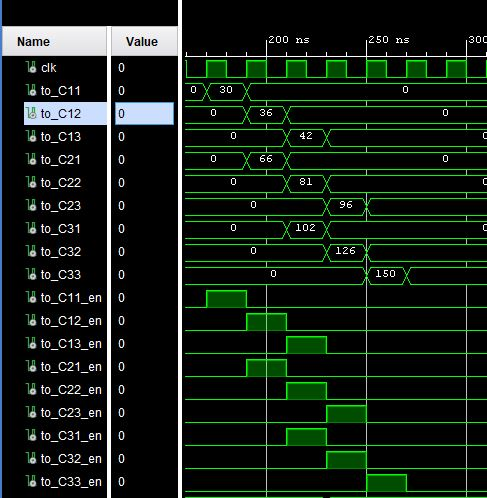
\includegraphics[width=15 cm , height= 12 cm]{Bilder/Simultionsergebnisse}
		\caption[]{Simulationsergebnis einer Matrixmultiplikation}
		\label{fig:Simultionsergebnisse}
	\end{figure}
\newpage

\begin{figure}[h!]
	\centering
	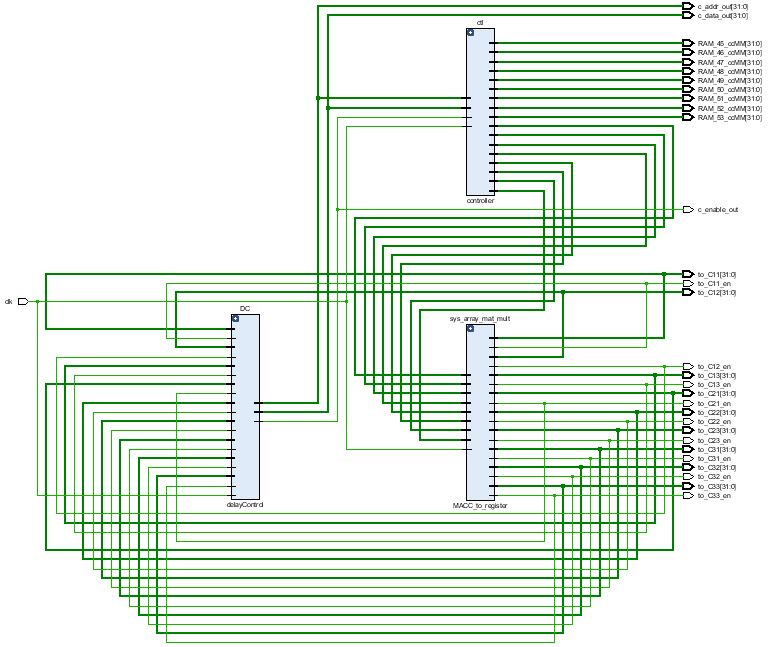
\includegraphics[width=15 cm , height= 12 cm]{Bilder/blockdiagram}
	\caption[Block Design von Matrixmultiplikation mit Systolic Array Architektur]{Es ist wegen Leitungen schwer zu sehen. In dem Design sind die oben vorgestellten Komponenten wie MAC (PE in MAC),RAM und Delay Controller.}
	\label{fig:blockdiagram}
\end{figure}


	\subsection{Zusammenfassung}\label{subsec:Zusammenfassung}
	In diesem Projekt wurde ein systolisches Array zur Berechnung der Matrixmultiplikation entworfen und implementiert. Die Vorteile des systolisches Arrays sind einfaches Design und zeitgleiche Operationen (Parallelität). Einige Nachteile sind, dass es nicht für allgemeine Anwendungen anwendbar ist, sondern eher für spezielle Zwecke geeignet ist, da die Organisation von PE (Processing element) zur Berechnung der Matrixelementen anpassen muss. Außerdem die Implementierung des systolichen Arrays ist beschränkt auf 3x3-Matrizen und die Dimension der Matrizen war nicht dynamisch, dass man am Anfang der Berechnung beliebig groß wählen darf. 

	
	
   		
    \chapter{Evaluation}\label{ch:Evaluation} %evaluation Experimentelle ergebnisse 
    Das Bildererkennungssystem ist ein sehr breites Forschungsgebiet und es geht nicht nur um Bilder zu erkennen, sondern auch deren Inhalt zu analysieren und verstehen. Heutzutage es ist ein sehr aktives Forschungsgebiet für Anwendungen von \textbf{C}onvolutional \textbf{N}eural \textbf{N}etwork (CNN). Die Aufgaben von solchen Anwendungen sind Klassifizierungen von Bilder, Segmentierung, Erkennung und Analyse von Szenen. \cite{AGuidetoConvolutional}\\
    Die meisten CNN Architekturen sind eingesetzt, um ein Objekt oder eine Person in einem Bild zu identifizieren oder das Label eines Objekts auszugeben.
    
    
    Die in \autoref{subsec:Beispiele von CNN Architekturen} vorgestellten Architekturen sind rechen- und speicherintensive Architekturen, die für Genauigkeiten von Ergebnissen mehr Energie brauchen. 
	
	
  

    \chapter{Ausblick}\label{ch:Ausblick}   
    In meiner Thesis werden zuerst die Grundlagen zum maschinellen Lernen erläuert und im folgenden die Strukturen der künstlichen neuronalen Netze betrachtet. Besonders wird die CNN-Architektur \textit{(convolutional neural network)} und ihr Entwicklungstrend betrachtet. Die Gemeinsamkeit von dieser vorgestellten Architekturen sind, dass die erste Entwurf in CNN sind wie z.B. LeNET oder die besondere Erfolge in ImageNet Large-Scale Visual Recognition Challenge (ILSVRC) bekommen haben. siehe \autoref{fig:GoogleNet} \autoref{fig:alexnet}
     
 
  
    
% =====================================================
% Bibliography
% ===================================================== 
\nocite{*}
%\addcontentsline{toc}{chapter}{Literaturverzeichnis, in ToC löschen}
%\addcontentsline{toc}{chapter}{Literature}
%\bibliographystyle{dinat}        % use a DIN style for the bibliography
%\bibliographystyle{plain}        % use a DIN style for the bibliography
%\bibliographystyle{abbrv}			%mit nummern in []
%\bibliographystyle{plain}			%mit nummern in []
%\bibliographystyle{alpha}			%3 Buchstaben + Jahr
\bibliographystyle{alphadin}

    % use external Bib-File, 
		\bibliography{99_bib/standardbib}	
		%https://www.rle.mit.edu/eems/wp-content/uploads/2016/02/eyeriss_isscc_2016_slides.pdf	
		\cleardoublepage
% =====================================================
% Appendix
% ===================================================== 
    \appendix

%    \input{95_anhang/anhang}
		\cleardoublepage

%    \listoftables
    %	\cleardoublepage
    \listoffigures
    %	\cleardoublepage
    \printindex
    %	\cleardoublepage
    \printnomenclature
    \renewcommand{\leftmark}{\uppercase{Abkürzungsverzeichnis}}
    	%\cleardoublepage

\end{document}

